\documentclass[journal]{IEEEtran}

\usepackage{adjustbox}
\usepackage{algorithm}
\usepackage{algpseudocode}
\usepackage{amsfonts}
\usepackage{amsmath}
\usepackage{amssymb}
\usepackage{amsthm}
\usepackage{bookmark}
\usepackage{booktabs}
\usepackage[american]{circuitikz}
\usepackage{cite}
\usepackage{fixmath}
\usepackage[acronym]{glossaries-extra}
\usepackage{hyperref}
\usepackage{import}
\usepackage{mathtools}
\usepackage{microtype}
\usepackage[short]{optidef}
\usepackage{pgfplots}
\usepackage{ragged2e}
\usepackage[subtle]{savetrees}
\usepackage{siunitx}
\usepackage{stfloats}
\usepackage[caption=false,font=footnotesize,subrefformat=parens,labelformat=parens]{subfig}
\usepackage{tabularx}
\usepackage{tikz}
\usepackage{xcolor}
% dark mode
% \usepackage{xcolor} \pagecolor[rgb]{0,0,0} \color[rgb]{1,1,1}

% amsthm
\newtheorem{proposition}{Proposition}
\newtheorem{remark}{Remark}

% siunitx
\DeclareSIUnit{\belm}{Bm}
\DeclareSIUnit{\dBm}{\deci\belm}
\DeclareSIUnit{\beli}{Bi}
\DeclareSIUnit{\dBi}{\deci\beli}

% PGF/TikZ
\usetikzlibrary{arrows,calc,matrix,patterns,plotmarks,positioning,shapes}
\usetikzlibrary{decorations.pathmorphing,decorations.pathreplacing,decorations.shapes,shapes.geometric}
\usepgfplotslibrary{groupplots,patchplots}
\pgfplotsset{compat=newest}

% tabularx, ragged2e
\newcolumntype{L}{>{\RaggedRight}X}
\newcolumntype{C}{>{\centering\arraybackslash}X}
\renewcommand\tabularxcolumn[1]{m{#1}}

% algpseudocode
\makeatletter
\renewcommand{\fnum@algorithm}{\fname@algorithm{} \thealgorithm:}
\makeatother
\algrenewcommand{\algorithmicrequire}{\textbf{Input:}}
\algrenewcommand{\algorithmicensure}{\textbf{Output:}}
\algrenewcommand{\algorithmicwhile}{\textbf{While}}
\algrenewcommand{\algorithmicend}{\textbf{End}}
\algrenewcommand{\algorithmicrepeat}{\textbf{Repeat}}
\algrenewcommand{\algorithmicuntil}{\textbf{Until}}
\algrenewcommand{\algorithmicdo}{}

% glossaries-extra
\setabbreviationstyle[acronym]{long-short}
\newacronym{af}{AF}{Amplify-and-Forward}
\newacronym{ambc}{AmBC}{Ambient Backscatter Communications}
\newacronym{ap}{AP}{Access Point}
\newacronym{awgn}{AWGN}{Additive White Gaussian Noise}
\newacronym{bcd}{BCD}{Block Coordinate Descent}
\newacronym{bc}{BackCom}{Backscatter Communications}
\newacronym{bibo}{BIBO}{Binary-Input Binary-Output}
\newacronym{bpcu}{\si{bpcu}}{bits per channel use}
\newacronym{bpsphz}{\si{bps/Hz}}{bits per second per Hertz}
\newacronym{cp}{CP}{Canonical Polyadic}
\newacronym{cr}{CR}{Cognitive Radio}
\newacronym{cscg}{CSCG}{Circularly Symmetric Complex Gaussian}
\newacronym{csi}{CSI}{Channel State Information}
\newacronym{df}{DF}{Decode-and-Forward}
\newacronym{dmc}{DMC}{Discrete Memoryless Channel}
\newacronym{dmtc}{DMTC}{Discrete Memoryless Thresholding Channel}
\newacronym{dmtmac}{DMTMAC}{Discrete Memoryless Thresholding Multiple Access Channel}
\newacronym{dp}{DP}{Dynamic Programming}
\newacronym{fdma}{FDMA}{Frequency-Division Multiple Access}
\newacronym{iid}{i.i.d.}{independent and identically distributed}
\newacronym{ioe}{IoE}{Internet of Everything}
\newacronym{iot}{IoT}{Internet of Things}
\newacronym{kkt}{KKT}{Karush-Kuhn-Tucker}
\newacronym{m2m}{M2M}{Machine to Machine}
\newacronym{mac}{MAC}{Multiple Access Channel}
\newacronym{mc}{MC}{Multiplication Coding}
\newacronym{miso}{MISO}{Multiple-Input Single-Output}
\newacronym{mimo}{MIMO}{Multiple-Input Multiple-Output}
\newacronym{ml}{ML}{Maximum-Likelihood}
\newacronym{mrt}{MRT}{Maximum Ratio Transmission}
\newacronym{noma}{NOMA}{Non-Orthogonal Multiple Access}
\newacronym{ofdm}{OFDM}{Orthogonal Frequency-Division Multiplexing}
\newacronym{pdf}{PDF}{Probability Density Function}
\newacronym{pgd}{PGD}{Projected Gradient Descent}
\newacronym{psk}{PSK}{Phase Shift Keying}
\newacronym{qam}{QAM}{Quadrature Amplitude Modulation}
\newacronym{qos}{QoS}{Quality of Service}
\newacronym{rf}{RF}{Radio-Frequency}
\newacronym{rfid}{RFID}{Radio-Frequency Identification}
\newacronym{ris}{RIS}{Reconfigurable Intelligent Surface}
\newacronym{sc}{SC}{Superposition Coding}
\newacronym{sic}{SIC}{Successive Interference Cancellation}
\newacronym{simo}{SIMO}{Single-Input Multiple-Output}
\newacronym{sinr}{SINR}{Signal-to-Interference-plus-Noise Ratio}
\newacronym{smawk}{SMAWK}{Shor-Moran-Aggarwal-Wilber-Klawe}
\newacronym{snr}{SNR}{Signal-to-Noise Ratio}
\newacronym{sr}{SR}{Symbiotic Radio}
\newacronym{swipt}{SWIPT}{Simultaneous Wireless Information and Power Transfer}
\newacronym{tdma}{TDMA}{Time-Division Multiple Access}
\newacronym{ue}{UE}{user}
\newacronym{wit}{WIT}{Wireless Information Transfer}
\newacronym{wpcn}{WPCN}{Wireless Powered Communication Network}
\newacronym{wpt}{WPT}{Wireless Power Transfer}
\newacronym{mbc}{MBC}{Monostatic Backscatter Communications}
\newacronym{bbc}{BBC}{Bistatic Backscatter Communications}
\newacronym{bls}{BLS}{Backtracking Line Search}
\newacronym{mrc}{MRC}{Maximal Ratio Combining}
\newacronym{sdma}{SDMA}{Space-Division Multiple Access}

\begin{document}
\title{RIScatter: Unifying\\Backscatter Communications, Symbiotic Radio, and Reconfigurable Intelligent Surface}
% \title{RIScatter: Unifying Backcatter Modulation and Passive Beamforming by Adaptive Input Distribution}
\author{
	\IEEEauthorblockN{
		Yang~Zhao,~\IEEEmembership{Member,~IEEE,}
		and~Bruno~Clerckx,~\IEEEmembership{Fellow,~IEEE}
	}
	\thanks{
		The authors are with the Department of Electrical and Electronic Engineering, Imperial College London, London SW7 2AZ, U.K. (e-mail: \{yang.zhao18, b.clerckx\}@imperial.ac.uk).
	}
}
\maketitle

\begin{abstract}
	% Scatterers can harvest energy from, modulate information over, and influence propagation of surrounding radio waves.
	% \gls{bc} varies object impedance to manipulate the magnitude, phase, and/or frequency of scattered signal to encode information and deliver within coverage.
	% \gls{bc} switches load impedance that manipulates the magnitude, phase, and/or frequency responses to modulate information onto the scattered signal.
	% \gls{bc} switches load impedance to manipulate the magnitude, phase, and/or frequency responses and modulate information onto the scattered signal.
	\gls{bc} switches device load impedance to manipulate the magnitude, phase, and/or frequency responses for information modulation on the scattered carrier.
	% \gls{sr} incorporates scatter nodes into active networks that recycle ambient signal to transmit self information and enhance legacy channel to the cooperative receiver.
	% \gls{sr} allows the transmission of a primary node using active radio carrying primary information and of a secondary node scattering information onto primary signal, and the reception of information of both nodes.
	% \gls{sr} introduces a passive scatterer that rides secondary information over the primary signal from an active transmitter, and employs a co-located receiver to sequentially decode both links.
	% \gls{sr} introduces a passive scatterer to ride secondary information over the primary radio from an active transmitter, and employs a co-located receiver to decode both links.
	% \gls{sr} introduces a passive scatterer to ride secondary information over the primary radio from an active transmitter and employs a co-located receiver to decode both links.
	\gls{sr} allows a passive scattering node to ride additional information over the primary radio emitted by an active transmitter, and employs a co-located receiver to decode both sources.
	% ride secondary information over the primary radio from an active transmitter and employs a co-located receiver to decode both links.
	% \gls{ris} adapts scattering antennas/programmable metamaterial to control wireless environment by varying signal strength in specific directions.
	% \gls{ris} programs antenna/metamaterial array that adjusts the scattering phase shifts to control signal strength in specific directions.
	\gls{ris} programs an antenna/metamaterial array to adjust the scattering phase shifts for signal propagation control in specific directions.
	% and control signal strength in specific directions.
	% In this paper, we depart from those concepts and introduce RIScatter as a new paradigm for future wireless networks.
	In this paper, we show how those three seemingly different technologies can be unified to leverage their benefits simultaneously into a single architecture called RIScatter.
	RIScatter is a new paradigm for future wireless networks and consists of multiple passive scattering nodes, whose reflection states can be adapted to partially engineer the wireless channel and partially modulate information onto the scattered wave.
	This contrasts with \gls{bc}/\gls{sr} (resp. \gls{ris}) where states are exclusively a function of information symbols (resp. \gls{csi}).
	The key principle in RIScatter is to render the probability distribution of reflection states as a joint function of the \gls{csi} and input information source, allowing universal hardware design and heterogeneous traffic control.
	% augmented \gls{qos} control.
	This enables RISscatter to softly bridge, generalize, and outperform \gls{bc}, \gls{sr}, \gls{ris}; boil down to any of those under specific reflection states; or evolve in a mixed setup.
	We reveal RIScatter provides a fundamental tradeoff that balances information modulation and channel reconfiguration capabilities in a flexible and mutualistic manner.
	% Instead of treating probability distribution of reflection states as equiprobable (as scattering source of \gls{bc}/\gls{sr}) or degenerate (as reflecting element of \gls{ris}), RIScatter nodes located at different places adapt the input distribution of passive scatterers based on link priority and \gls{csi}, balancing information encoding and channel reconfiguration in a flexible and mutualistic manner.
	% RIScatter receiver semi-coherently decodes all nodes from accumulated energy, determines primary equivalent channel over reflection pattern, then coherently decodes the primary link under enhanced multipath.
	% It reduces the complexity of cooperative decoding while preserves the benefits of backscatter modulation and passive beamforming.
	% To accommodate signal characteristics, we also propose a low-complexity RIScatter receiver that preserves the aforementioned benefits.
	% Using shared spectrum, energy, and infrastructures, RIScatter is a general and powerful transmit-assist protocol that unifies \gls{bc}, \gls{ris} and \gls{sr} with universal hardware design and augmented \gls{qos} control.
	% We consider an application scenario where a multi-antenna \gls{ap} serves a single-antenna user surrounded by multiple RIScatter nodes, and characterize the achievable primary-total-backscatter rate region by designing input distribution at the nodes, active beamforming at the \gls{ap}, and backscatter decision regions at the user.
	An application scenario is considered where a multi-antenna \gls{ap} serves a single-antenna user surrounded by multiple RIScatter nodes, and the achievable primary-total-backscatter rate region is characterized by optimizing input distribution at the nodes, active beamforming at the \gls{ap}, and backscatter decision regions at the user.
	% Simulation results demonstrate RIScatter nodes can flexibly control the transmit-assist tradeoff via smart input distribution design.
	% Simulation results demonstrate RIScatter can flexibly control the tradeoff between backscatter modulation and passive beamforming via smart input distribution design, which outperforms \gls{bc}, \gls{sr}, and \gls{ris}.
	Simulation results demonstrate RIScatter can exploit the additional propagation paths to provide a smooth transition between backscatter modulation and passive beamforming via smart input distribution design, which includes \gls{bc}, \gls{sr}, \gls{ris} as special cases.
	% Simulation results demonstrate RIScatter can exploit smart input distribution design to provide a smooth transition between backscatter modulation and passive beamforming, which outperforms \gls{bc}, \gls{sr}, and \gls{ris}.
\end{abstract}

\glsresetall

\begin{section}{Introduction}
	\begin{subsection}{Fundamentals}
		\IEEEPARstart{F}{uture} wireless network is envisioned to provide high throughput, uniform coverage, pervasive connectivity, heterogeneous control, and cognitive intelligence for trillions of portable devices.
		As an emerging low-power communication technique, \gls{bc} separates conventional transmitter into a \gls{rf} carrier emitter with power-hungry elements (e.g., synthesizer and amplifier) and an information-bearing node with power-efficient components (e.g., harvester and modulator) \cite{Boyer2014}.
		The node harvests energy from impinging wave and embeds information over scattered signal in a sustainable and controllable manner.
		% The backscatter reader can be either co-located or separated with the carrier emitter, known as monostatic and bistatic \gls{bc}.
		The backscatter reader can be either co-located or separated with the carrier emitter, known as \gls{mbc} and \gls{bbc} in Fig. \subref*{fi:mbc} and \subref*{fi:bbc}, respectively.
		Its applications such as \gls{rfid} \cite{Dobkin2012,Landt2005} and passive sensor network \cite{Vannucci2008,Assimonis2016} have been extensively researched, standardized, and commercialized to support \gls{iot} and \gls{m2m} networks.
		% ? Specifically, a dedicated emitter generates a sinusoidal carrier at reserved frequency, and \gls{rfid} tags reports their identifier to a nearby \gls{rfid} reader.
		% ? With the upsurge of wireless devices and the downtrend of circuit power consumption, \gls{rfid} has experienced great success in \gls{ioe} and \gls{m2m} networks.
		However, traditional \gls{bc} nodes only respond when externally inquired.
		In \gls{ambc} \cite{Liu2013b}, interactive nodes recycle ambient signals from legacy transmitters (e.g., radio, television and Wi-Fi) to harvest energy and establish connections.
		As illustrated in Fig. \subref*{fi:ambc}, it eliminates the need of dedicated power supply, carrier emitter and frequency spectrum, bringing more opportunities to low-power communications.
		To combat the strong direct-link interference of \gls{ambc}, \cite{Yang2018} proposed a co-located receiver that cooperatively decodes both primary (legacy) and backscatter links.
		% The authors evaluated the error performance of \gls{ml}, linear, and \gls{sic} detectors for flat fading channel, and proposed a low-complexity detector for frequency-selective fading channel.
		The concept of cooperative \gls{ambc} was further refined as \gls{sr} in Fig. \subref*{fi:sr} that cognitively incorporates \gls{ambc} with existing systems \cite{Liang2020}.
		% In \gls{sr}, the primary transmitter generates active radio carrying primary information, the backscatter node modulates own information onto the scattered wave, and the co-located receiver decodes both links from two propagation paths.
		% In \gls{sr}, the primary transmitter generates active radio and modulates primary information, the passive node scatters incoming wave and superimposes backscatter information, and the co-located receiver decodes both links from two propagation paths.
		In \gls{sr}, the primary transmitter generates active radio and modulates primary information, the passive node scatters incoming wave and superimposes backscatter information, while the co-located receiver decodes both links from both propagation paths.
		% The direct transmitter-receiver path only convey
		% The component over the direct transmitter-receiver path only
		% The direct transmitter-receiver path contains primary information, and the cascaded transmitter-node-receiver path preserves both information in a superimposed manner.
		% The direct transmitter-receiver path only contains modulated primary signal while the cascaded transmitter-node-receiver path preserves superimposed signal
		% both thanks to signal characteristics.
		% Such a coexistence was further classified into commensal, parasitic, and competitive relationships based on link priority \cite{Guo2019b}, and their instantaneous rates, optimal power allocations, and outage probabilities were subsequently derived in \cite{Guo2019b,Ding2020}.
		% However, one important issue of \gls{sr} is practical cooperative decoding design.
		% Due to physical constraints at the load-switching modulator, backscatter symbol period is typically longer than primary.
		% Ideal joint \gls{ml} decoding achieves optimal performance with prohibitive computational complexity \cite{Yang2018,Liang2020,Zhang2022}.
		% For sequential decoding from primary to backscatter, \cite{Long2020a} pointed out the randomness from backscatter modulation can be modelled as either interference or channel uncertainty, depending on the symbol period ratio.
		% The authors concluded if this ratio is sufficiently large, the non-coherent primary achievable rate would asymptotically approach its coherent counterpart.
		% This motivated \cite{Long2020a,Liang2020,Guo2019b,Ding2020,Zhou2019a,Wu2021a,Xu2021a,Yang2021a,Yang2018,Han2021,Zhang2022} to first decode the primary link, perform \gls{sic}, then decode the backscatter link.
		% However, the advantage of \gls{sic} is questionable because 1) sufficiently large symbol period ratio is assumed in primary rate analysis and constraints backscatter rate; 2) backscatter pattern and signal characteristics are not fully exploited; 3) non-coherent primary encoding is required at the transmitter, while re-encoding, precoding, and subtraction are required at the receiver; 4) primary and backscatter symbols are superimposed by multiplication instead of superposition.
		% Another open issue for \gls{sr} is backscatter multiple access.
		% \cite{Xu2021a} extended \gls{sic} to multi-node scenario and proposed a backscatter \gls{noma}-based \gls{sr} with decoding order following backscatter signal strength.
		% However, its performance deteriorates fast when the number of nodes increases.
		% Backscatter \gls{tdma} was also evaluated in \cite{Yang2021a}, where each node transmits information during dedicated slot and harvests energy during others.
		% It enhances energy efficiency by transmission time and reflection ratio optimization, but requires regular feedback to passive nodes and incurs high coordination cost.
		% \cite{Vougioukas2019} controls the load-switching speed at nodes to shift the scattered signal to desired frequency bands.
		% This enables backscatter \gls{fdma} at the cost of extra bandwidth and higher power consumption.
		% To reduce coordination between passive nodes, \cite{Han2021} proposed a random code-assisted multiple access for \gls{sr} and evaluated the asymptotic \gls{sinr} using random matrix theory.
		% However, it suffers from imperfect synchronization and the near-far problem.
		On the other hand, \gls{ris} in Fig. \subref*{fi:ris} is a promising technology that evolves wireless propagation environment using numerous passive reflecting elements (e.g., scattering antenna or programmable metamaterial) with adjustable amplitudes and/or phases \cite{Wu2021b}.
		With proper phase shift design, the scattered components can add constructively/destructively with the direct component for signal enhancement/interference suppression.
		% Compared with scattering nodes of \gls{bc}/\gls{sr}, \gls{ris} elements embed no additional information and use deterministic reflection pattern priorly known at the transmitter and receiver.
		Compared with scattering nodes of \gls{bc}/\gls{sr}, \gls{ris} elements embed no additional information and use fixed reflection pattern over time, which can be optimized and fed back to the transmitter and receiver during coordination phase.
		% , which can be priorly known at the transmitter and receiver.
		% contain no additional information


		% employ deterministic reflection pattern over time that contains no information

		% and priorly known at transmitter and receiver.
		% This motivated the use of fixed reflection coefficients during each channel block to improve communication, sensing, and power performances \cite{Wu2018,Zhang2019a,Lin2022,Liu2022,Feng2022,Zhao2022}.
		% The concept of dynamic \gls{ris}, namely choosing independent reflection coefficients over different time slots within channel block, was first considered for resource blocks of \gls{ofdm} systems, then extended to power and information phases of \gls{wpcn} \cite{Wu2021,Wu2021d,Hua2022a}.
		% Dynamic \gls{ris} provides artificial channel diversity and flexible resource allocation, but misses the opportunity to encode its own message.
		% From an information-theoretic perspective, \cite{Karasik2020} reported using \gls{ris} as an auxiliary passive beamforming device to maximize the \gls{snr} is generally rate-suboptimal for finite input constellations.
		% Instead, joint transmitter-\gls{ris} encoding achieves the capacity of \gls{ris}-aided channel, and layered encoding with \gls{sic} decoding (i.e., \gls{sic}-based \gls{sr}) can outperform pure passive beamforming at high \gls{snr}.
		% It inspired \cite{Liu2019d,Bereyhi2020,Xu2020b,Zhang2021d,Hu2021b,Hua2022,Basar2020,Ma2020a,Yuan2021,Hu2021a} to employ \gls{ris} also as an information source to combine passive beamforming and backscatter modulation in the overall reflection pattern.
		% In particular, \emph{symbol level precoding} maps backscatter symbols to \gls{ris} coefficient sets optimized for detection \cite{Liu2019d,Bereyhi2020}, \emph{overlay modulation} superposes information-bearing symbols over a common auxiliary matrix \cite{Xu2020b,Zhang2021d,Hu2021b,Hua2022}, \emph{spatial modulation} switches between reflection coefficient sets that maximize \gls{snr} at different receive antennas \cite{Basar2020,Ma2020a,Yuan2021}, and \emph{index modulation} divides \gls{ris} into reflection elements for passive beamforming and information elements for on-off modulation \cite{Hu2021a}.
		% However, those \gls{ris}-empowered \gls{bc}/\gls{sr} designs involve advanced hardware architecture, high optimization complexity, and additional control overhead.

		\begin{figure}[!t]
			\centering
			\subfloat[\gls{mbc}]{
				\resizebox{0.48\linewidth}{!}{
					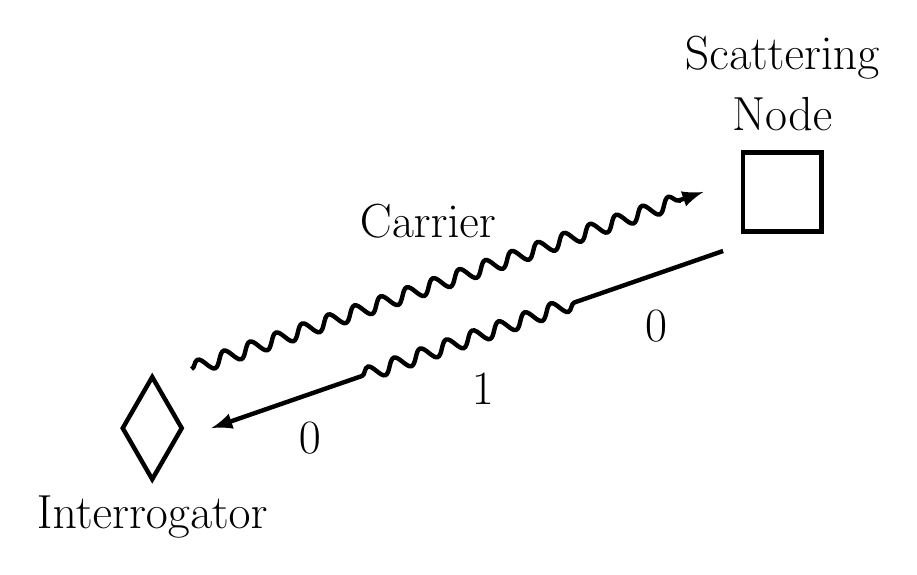
\begin{tikzpicture}[font=\LARGE,every node/.style={draw,ultra thick},every path/.style={ultra thick},every text node part/.style={align=center}]
	\node at (0,0) [kite,minimum size=0.75cm,kite vertex angles=60] {};
	\node at (8,3) [rectangle,minimum size=1cm] {};

	\node[draw=none] at (0,-1.125) {Interrogator};
	\node[draw=none] at (8,4.375) {Scattering\\Node};

	\draw[decorate,decoration={snake,post length=2.5mm},-latex] (0.5,0.75) -- (7,3);
	\draw[decorate,decoration={snake,pre length=2cm,post length=2cm},-latex] (7.25,2.25) -- (0.75,0);

	\node[draw=none] at (3.5,2.625) {Carrier};
	\node[draw=none] at (4.2,0.5) {1};
	\node[draw=none] at (2,-0.125) {0};
	\node[draw=none] at (6.4,1.3) {0};
\end{tikzpicture}

				}
				\label{fi:mbc}
			}
			\subfloat[\gls{bbc}]{
				\resizebox{0.48\linewidth}{!}{
					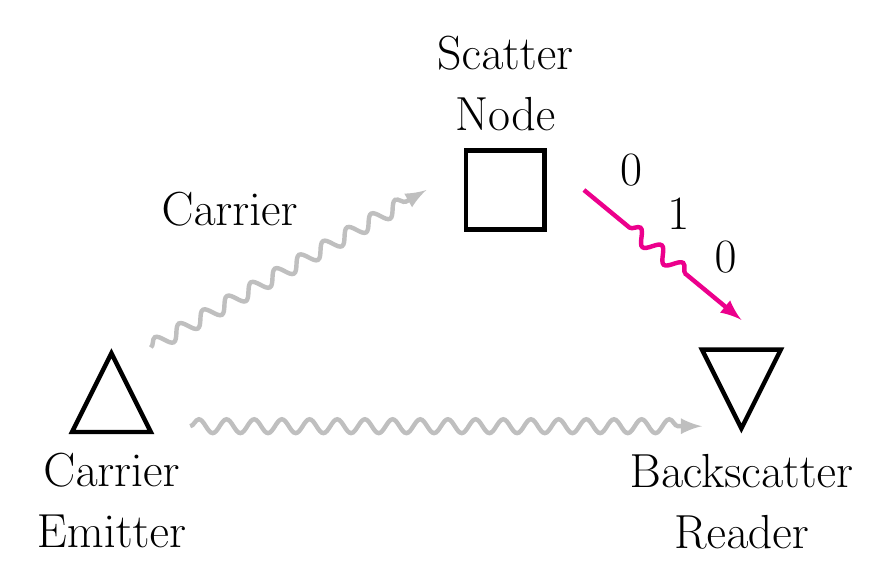
\begin{tikzpicture}[font=\LARGE,every node/.style={draw,ultra thick},every path/.style={ultra thick},every text node part/.style={align=center}]
	\node at (0,0) [isosceles triangle,isosceles triangle stretches,shape border rotate=+90,minimum size=1cm,minimum height=1cm,anchor=north] {};
	\node at (5,2) [rectangle,minimum size=1cm] {};
	\node at (8,0) [isosceles triangle,isosceles triangle stretches,shape border rotate=+270,minimum size=1cm,minimum height=1cm,anchor=north] {};

	\node[draw=none] at (0,-1.95) {Carrier\\Emitter};
	\node[draw=none] at (5,3.35) {Scatter\\Node};
	\node[draw=none] at (8,-1.95) {Backscatter\\Reader};

	\draw[lightgray,decorate,decoration={snake,post length=2.5mm},-latex] (1,-1) -- (7.5,-1);
	\draw[lightgray,decorate,decoration={snake,post length=2.5mm},-latex] (0.5,0) -- (4,2);
	\draw[magenta,decorate,decoration={snake,pre length=7.5mm,post length=7.5mm},-latex] (6,2) -- (8,0.35);

	\node[draw=none] at (1.5,1.75) {Carrier};
	\node[draw=none] at (7.2,1.7) {1};
	\node[draw=none] at (6.6,2.25) {0};
	\node[draw=none] at (7.8,1.15) {0};
\end{tikzpicture}

				}
				\label{fi:bbc}
			}
			\\
			\subfloat[\gls{ambc}]{
				\resizebox{0.48\linewidth}{!}{
					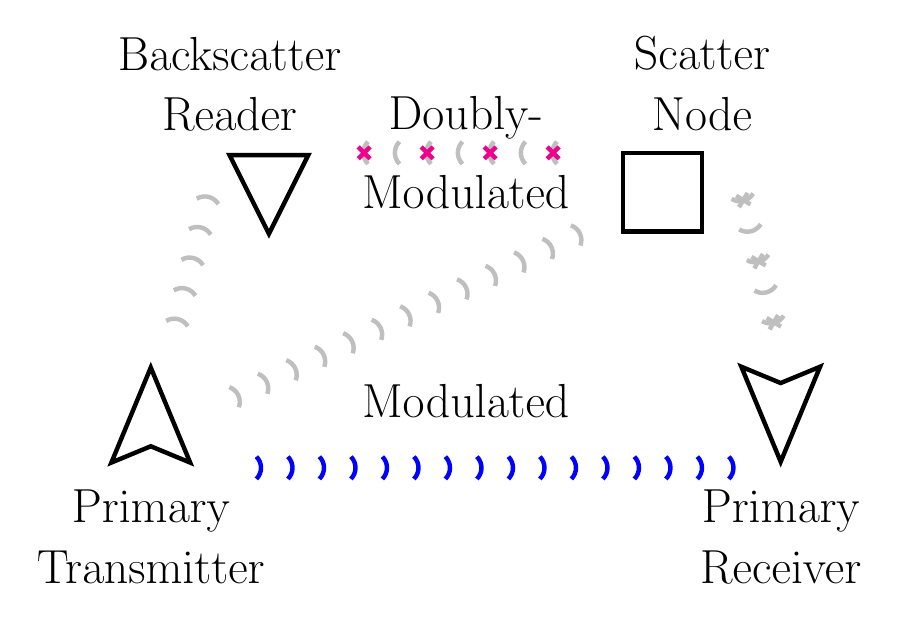
\begin{tikzpicture}[font=\LARGE,every node/.style={draw,ultra thick},every path/.style={ultra thick},every text node part/.style={align=center}]
	\node at (0,0) [dart,shape border rotate=90,minimum width=1cm] {};
	\node at (1.5,3.5) [isosceles triangle,isosceles triangle stretches,shape border rotate=+270,minimum size=1cm,minimum height=1cm,anchor=north] {};
	\node at (6.5,3) [rectangle,minimum size=1cm] {};
	\node at (8,0.35) [dart,shape border rotate=270,minimum width=1cm] {};

	\node[draw=none] at (0,-1.375) {Primary\\Transmitter};
	\node[draw=none] at (1,4.375) {Backscatter\\Reader};
	\node[draw=none] at (7,4.375) {Scatter\\Node};
	\node[draw=none] at (8,-1.375) {Primary\\Receiver};

	\draw[blue,decorate,decoration={waves,segment length=4mm,radius=2mm}] (1,-0.5) -- (7.5,-0.5);
	\draw[lightgray,decorate,decoration={waves,segment length=4mm,radius=2mm}] (0.25,1) -- (0.75,3);
	\draw[lightgray,decorate,decoration={waves,segment length=4mm,radius=2mm}] (0.75,0.25) -- (5.5,2.5);
	\draw[lightgray,decorate,decoration={waves,segment length=4mm,radius=2mm}] (5.5,3.5) -- (2.5,3.5);
	\draw[magenta,decorate,decoration={crosses,segment length=8mm,shape size=1.5mm}] (5.11,3.5) -- (2.5,3.5);
	\draw[lightgray,decorate,decoration={waves,segment length=4mm,radius=2mm}] (7.43,3.28) -- (8,1);
	\draw[lightgray,decorate,decoration={crosses,segment length=8mm,shape size=1.5mm}] (7.525,2.9) -- (8,1);

	\node[draw=none] at (4,0.35) {Modulated};
	\node[draw=none] at (4,3.95) {Doubly-};
	\node[draw=none] at (4,3) {Modulated};
\end{tikzpicture}

				}
				\label{fi:ambc}
			}
			\subfloat[\gls{sr}]{
				\resizebox{0.48\linewidth}{!}{
					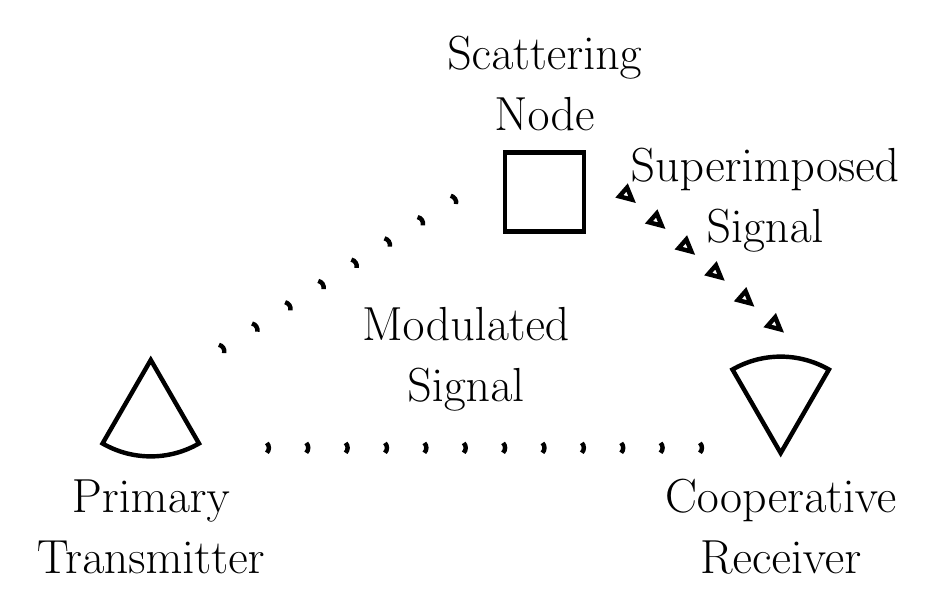
\begin{tikzpicture}[font=\LARGE,every node/.style={draw,ultra thick},every path/.style={ultra thick},every text node part/.style={align=center}]
	\node at (0,0) [circular sector,shape border rotate=90,minimum width=2cm] {};
	\node at (5,3) [rectangle,minimum size=1cm] {};
	\node at (8,0.55) [circular sector,shape border rotate=270,minimum width=2cm] {};

	\node[draw=none] at (0,-1.25) {Primary\\Transmitter};
	\node[draw=none] at (5,4.375) {Scattering\\Node};
	\node[draw=none] at (8,-1.25) {Cooperative\\Receiver};

	\draw[decorate,decoration={waves,segment length=5mm}] (1,-0.25) -- (7.375,-0.25);
	\draw[decorate,decoration={waves,segment length=5mm}] (0.5,0.75) -- (4,3);
	\draw[decorate,decoration={triangles,segment length=5mm,shape size=1.5mm}] (6,3) -- (8,1.25);

	\node[draw=none] at (4,0.875) {Modulated\\Signal};
	\node[draw=none] at (7.8,2.9) {Superimposed\\Signal};
\end{tikzpicture}

				}
				\label{fi:sr}
			}
			\\
			\subfloat[\gls{ris}]{
				\resizebox{0.48\linewidth}{!}{
					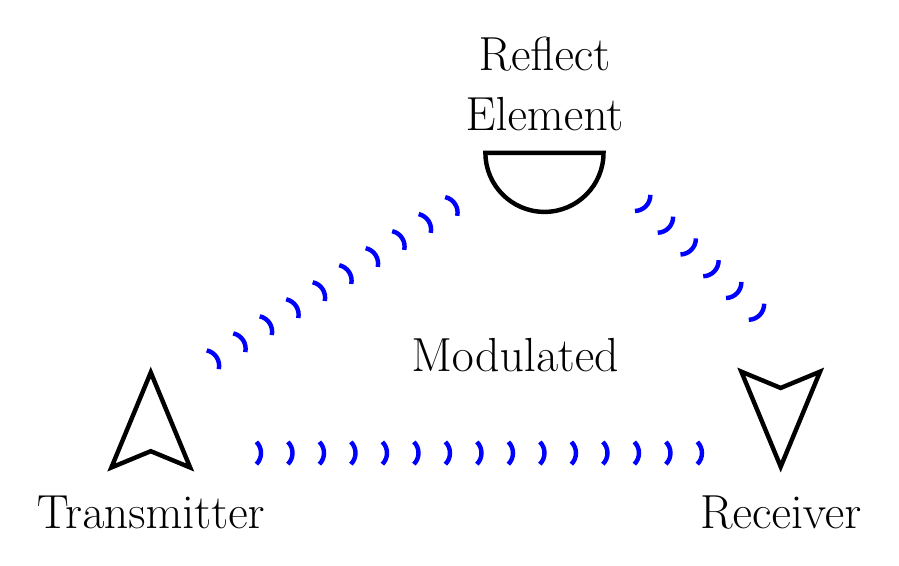
\begin{tikzpicture}[font=\LARGE,every node/.style={draw,ultra thick},every path/.style={ultra thick},every text node part/.style={align=center}]
	\node at (0,0) [dart,shape border rotate=90,minimum width=1cm] {};
	\node at (5,3.25) [semicircle,shape border rotate=180,minimum width=1.5cm] {};
	\node at (8,0.35) [dart,shape border rotate=270,minimum width=1cm] {};

	\node[draw=none] at (0,-1) {Transmitter};
	\node[draw=none] at (5,4.4375) {Reflect\\Element};
	\node[draw=none] at (8,-1) {Receiver};

	\draw[blue,decorate,decoration={waves,segment length=4mm,radius=2mm}] (1,-0.25) -- (7.375,-0.25);
	\draw[blue,decorate,decoration={waves,segment length=4mm,radius=2mm}] (0.5,0.75) -- (4,3);
	\draw[blue,decorate,decoration={waves,segment length=4mm,radius=2mm}] (6,3.1625) -- (8,1.25);

	\node[draw=none] at (4.625,1) {Modulated};
\end{tikzpicture}

				}
				\label{fi:ris}
			}
			\subfloat[RIScatter]{
				\resizebox{0.48\linewidth}{!}{
					\begin{tikzpicture}[every node/.style={draw}]
	\node at (0,0) [dart,shape border rotate=90,minimum width=1cm] {};
	\node at (7,4) [circle,minimum size=1cm] {};
	\node at (10,0.35) [dart,shape border rotate=270,minimum width=1cm] {};

	\node[draw=none] at (0,-0.75) {Primary Transmitter};
	\node[draw=none] at (7,5) {RIScatter Node};
	\node[draw=none] at (10,-0.75) {Cooperative Receiver};
	\draw[loosely dashed,-latex] (0.75,0) -- (9.25,0);
	\draw[loosely dashed,-latex] (0.5,0.5) -- (6.25,4);
	\draw[dashdotted,-latex] (7.75,4) -- (10,1);
\end{tikzpicture}

				}
				\label{fi:riscatter}
			}
			\caption{
				Illustration of scattering applications.
				% Paradigms for various scattering applications.
			}
			\label{fi:scatter_comparison}
		\end{figure}
	\end{subsection}

	\begin{table*}[]
		\caption{Comparison of Scattering Applications}
		\begin{tabularx}{\textwidth}{CCCCCCC}
			\toprule
			                              & \gls{mbc}                 & \gls{bbc}                 & \gls{ambc}                                      & \gls{sr}                                     & \gls{ris}                               & RIScatter                                         \\ \midrule
			Coexisting systems            & 1                         & 1                         & 2 (competitive)                                 & 2 (?ly collaborative)                        & 1                                       & 2 (adaptively collaborative)                      \\ \midrule
			Scatterer contribution        & Backscatter modulation    & Backscatter modulation    & Backscatter modulation and primary interference & Backscatter modulation and primary multipath & Passive beamforming                     & Backscatter modulation and passive beamforming    \\ \midrule
			Cooperative transmission      & ---                       & ---                       & No                                              & Active beamforming                           & ---                                     & Active beamforming and smart reflection           \\ \midrule
			Cooperative reception         & ---                       & ---                       & No (separated receivers)                        & Joint detection or \gls{sic}                 & ---                                     & Backscatter detection as primary channel training \\ \midrule
			Primary detection             & ---                       & ---                       & Semi-coherent                                   & Coherent or semi-coherent                    & Coherent                                & Coherent                                          \\ \midrule
			Backscatter detection         & Coherent                  & Coherent                  & Semi-coherent or noncoherent                    & Coherent                                     & ---                                     & Semi-coherent                                     \\ \midrule
			Reflection state distribution & Equiprobable (line-coded) & Equiprobable (line-coded) & Equiprobable (line-coded)                       & Equiprobable or Gaussian                     & Degenerate (\gls{csi}-adaptive)         & Flexible (\gls{csi}- and link priority-adaptive)  \\ \midrule
			Load-switching frequency      & Fast or slow              & Fast or slow              & Fast or slow                                    & Slow                                         & Slow (dynamic) or very slow (blockwise) & Fast or slow                                      \\ \bottomrule
		\end{tabularx}
	\end{table*}

	\begin{subsection}{Related Works}
		Similar to \gls{cr}, the coexistence of primary and backscatter links in \gls{sr} can be classified into commensal, parasitic, and competitive relationships, whose instantaneous rates, power schemes, and outage probabilities were acquired in \cite{Guo2019b,Ding2020}.
		To evaluate the performance of cooperative \gls{sr} receivers, \cite{Yang2018} derived the bit error rates of \gls{ml}, linear, and \gls{sic} detectors for flat fading channels, then proposed a low-complexity detector for frequency-selective fading channels.
		However, it assumed equal symbol period of both links with perfect synchronization, which is impractical due to the load-switching speed constraint.
		Although joint \gls{ml} decoding achieves the optimal detection performance for arbitrary backscatter-over-primary symbol period ratio, the computational complexity is prohibitive especially for high-order constellations \cite{Yang2018,Liang2020,Zhang2022}.
		For sequential primary-backscatter decoding, the randomness of backscatter modulation can be modelled as either interference or channel uncertainty, depending on the symbol period ratio \cite{Long2020a}.
		If this ratio is sufficiently large, the authors proved the non-coherent primary achievable rate would approach its coherent counterpart asymptotically.
		This motivated \cite{Long2020a,Liang2020,Guo2019b,Ding2020,Zhou2019a,Wu2021a,Xu2021a,Yang2021a,Yang2018,Han2021,Zhang2022} to perform \gls{sic} from primary to backscatter links.
		However, the advantages of such \gls{sic} remain questionable as
		1) primary rate analysis is backed by long backscatter symbol period that constrains backscatter rate;
		2) reflection pattern and signal characteristics are not fully exploited;
		3) non-coherent primary encoding is required at the transmitter while re-encoding, precoding and subtraction are required at the receiver;
		4) primary and backscatter symbols are superimposed by multiplication instead of superposition.

		Another open issue for \gls{bc} and \gls{sr} is node multiple access.
		\cite{Xu2021a} proposed a \gls{noma}-based \gls{sr} with \gls{sic} order in backscatter equivalent channel strength, whose performance deteriorates fast when the number of nodes increases.
		\gls{tdma}-based \gls{sr} was also considered in \cite{Yang2021a} where each node transmits information during its dedicated slot and harvests energy during others.
		It allows adaptive transmission time and reflection ratio optimization, but requires regular feedback and incurs high coordination cost.
		\cite{Vougioukas2019} controls the load-switching speed to shift the scattered signal to the desired frequency band.
		This enables backscatter \gls{fdma} at the cost of extra bandwidth and higher power consumption.
		To reduce coordination burden for passive nodes, \cite{Han2021} proposed a random code-assisted multiple access for \gls{sr} and evaluated the asymptotic \gls{sinr} using random matrix theory.
		However, this code-domain solution suffers from imperfect synchronization and the near-far problem.

		Conventional \gls{ris} design with fixed reflection coefficients during each channel block has been extensively studied in communication, sensing, and power literatures \cite{Wu2018,Zhang2019a,Lin2022,Liu2022,Feng2022,Zhao2022}.
		In contrast, dynamic \gls{ris} that chooses independent reflection coefficients over different time slots has gained recent attentions in multi-user and multi-purpose wireless networks.
		The concept was first considered for resource blocks of \gls{ofdm} systems, then extended to power and information phases of \gls{wpcn} \cite{Wu2021,Wu2021d,Hua2022a}.
		Dynamic \gls{ris} provides artificial channel diversity and flexible resource allocation, but misses the opportunity to encode its own message.
		From an information-theoretic perspective, \cite{Karasik2020} reported using \gls{ris} as an auxiliary passive beamforming device to maximize the \gls{snr} is generally rate-suboptimal for finite input constellations.
		Instead, joint transmitter-\gls{ris} encoding achieves the capacity of \gls{ris}-aided channel, and layered encoding with \gls{sic} decoding (i.e., \gls{sic}-based \gls{sr}) can outperform pure passive beamforming at high \gls{snr}.
		It inspired \cite{Liu2019d,Bereyhi2020,Xu2020b,Zhang2021d,Hu2021b,Hua2022,Basar2020,Ma2020a,Yuan2021,Hu2021a} to employ \gls{ris} also as an information source to combine passive beamforming and backscatter modulation in the overall reflection pattern.
		In particular, \emph{symbol level precoding} maps backscatter symbols to optimized \gls{ris} coefficient sets \cite{Liu2019d,Bereyhi2020}, \emph{overlay modulation} superposes information-bearing symbols over a common auxiliary matrix \cite{Xu2020b,Zhang2021d,Hu2021b,Hua2022}, \emph{spatial modulation} switches between reflection coefficient sets that maximize \gls{snr} at different receive antennas \cite{Basar2020,Ma2020a,Yuan2021}, and \emph{index modulation} divides \gls{ris} into reflection elements for passive beamforming and information elements for on-off modulation \cite{Hu2021a}.
		However, those \gls{ris}-empowered \gls{bc}/\gls{sr} designs involve advanced hardware architecture, high optimization complexity, and additional control overhead.
		Besides, all relevant literatures assumed at backscatter information sources either Gaussian codebook \cite{Guo2019b,Ding2020,Long2020a,Zhou2019a,Wu2021a,Xu2021a,Yang2021a,Hu2021b} or finite equiprobable inputs \cite{Yang2018,Liang2020,Han2021,Zhang2022,Liu2019d,Bereyhi2020,Xu2020b,Zhang2021d,Hua2022,Basar2020,Ma2020a,Yuan2021,Hu2021a}.
		The former is impractical for passive backscatter devices, while the latter does not fully exploit reflection pattern and \gls{csi}.
	\end{subsection}

	% TODO why not use metamaterial? because high computational complexity and expectations of freedom (flexibility, reliability)
	% TODO cooperative input design can be used for co-located RIScatter nodes.
	% TODO hardward to modulate using RIS is already available.
	% TODO RIScatter: enhance backscatter signal difference (suppress primary interference) or primary signal strength.
	% TODO For Backscatter community: why not adaptive channel coding? For RIS community: why not add randomness for modulation?
	% TODO RIS involves nonlinear circuits (e.g., diodes) and impedance design (i.e., perfect mismatching) is tricky for continuous phase shift; discrete candidate set is preferred (2-3 bits optimal)
	% TODO Redefine RIS using book
	% TODO Using RIS to encode is not very interesting as controller is anyway usable
	% TODO Wi-Fi sampling rate 20 MHz (symbol period 50 nS), RFID symbol rate/load switching speed 100s KHz to 10s MHz [Backscatter Communications], fast load switching speed is key for high data rate - symbol ratio is not very large
	% TODO Beamforming can cancel direct interference to avoid the collapse of non-coherent energy detection and enlarge energy gap.
	% ? [Reconfigurable Intelligent Surface-Assisted Ambient Backscatter Communications Experimental Assessment]the authors of [5] show that, even in line-of-sight (LOS), the interferences and the desired signal can combine in such a way that the received signals at the reader side in the two states are close in power and only differ by their phases
	% TODO Input probability distribution for discrete-value reflection (backscatter), constellation design for continue-value reflection (RIS)
	% TODO convergence
	% TODO channel coding: general non-adaptive (book) adaptive (DMC)
	% ? [Turbocharging] Since averaging must be done over a significant period of time to smooth out the variation in the TV transmissions, averaging does not allow rates much higher than 10 kbps [24].
	% TODO mu-code: use multiple Rxs for noncoherent direct interference cancellation (instead of receive diversity)
	% TODO backscatter modulation <-> passive beamforming; add adaptive channel coding over (NRZ) line coding.
	% TODO semicoherent: known CSI, unknown primary/backscatter symbols
	% TODO initialization, convergence
	% TODO Base e, use 2 in simulation


	% To the best of our knowledge, all relevant literatures assumed at backscatter information sources either Gaussian codebook \cite{Guo2019b,Ding2020,Long2020a,Zhou2019a,Wu2021a,Xu2021a,Yang2021a,Hu2021b} or finite equiprobable inputs \cite{Yang2018,Liang2020,Han2021,Zhang2022,Liu2019d,Bereyhi2020,Xu2020b,Zhang2021d,Hua2022,Basar2020,Ma2020a,Yuan2021,Hu2021a}.
	% The former is impractical for passive backscatter devices, while the latter does not fully exploit reflection pattern and \gls{csi}.
	\begin{subsection}{Contributions}
		We introduce RIScatter that generalizes \gls{bc}, \gls{sr}, and \gls{ris} to manipulate the transmit-assist tradeoff via smart input distribution and practical receiver design.
		The paradigm of RIScatter is presented in Fig. \subref*{fi:riscatter}, and the contributions of this paper are summarized as follows.

		\emph{First,} we propose RIScatter nodes to adapt the input probability distribution of a finite-state passive scatter device based on link priority and \gls{csi}.
		The reflection pattern over time is no longer fully random or deterministic, but can be flexibly distributed to unify and balance backscatter modulation with passive beamforming.
		Scattering source of \gls{bc}/\gls{sr} and reflecting element of \gls{ris} can be regarded as its extreme cases, where the input distribution boils down to equiprobable and degenerate, respectively.
		Like aforementioned \gls{ris}-empowered \gls{bc}/\gls{sr} schemes, the passive nodes require regular coordination with ambient devices, but the advantages are
		1) RIScatter nodes can be built over universal load-switching scatterers instead of composite metamaterial;
		2) backscatter modulation and passive beamforming are unified by adaptive input distribution instead of advanced hardware architecture;
		3) optimization cost of input distribution is much lower than that of \gls{ris} reflection coefficients;
		4) adaptive backscatter channel coding can exploit \gls{csi} to achieve higher instantaneous rate than conventional equiprobable line coding in \gls{bc}/\gls{sr};
		5) the potentially dispersed characteristics of RIScatter nodes (and legacy users) avoids the development optimization and allows uniformly good performance for both links.

		\emph{Second,} we propose a practical RIScatter receiver that semi-coherently decodes RIScatter nodes from the received energy per backscatter block, re-encodes for their reflection patterns, retrieves primary equivalent channel as if dynamic passive beamforming, then coherently decodes the primary link under the enhanced multipath.
		The proposed receiver
		1) preserves the benefits of backscatter modulation and passive beamforming;
		2) enjoys lower computational and operational complexities than joint \gls{ml} and \gls{sic} schemes;
		3) accommodates the link difference and suits for diverse symbol period ratios;
		4) requires minor modification over legacy hardware.

		\emph{Third,} we consider an application scenario where multiple RIScatter nodes ride over a point-to-point \gls{miso} transmission, performing backscatter modulation and passive beamforming to a nearby user using shared spectrum, energy, and infrastructures.
		To investigate how RIScatter unifies \gls{bc}, \gls{sr} and \gls{ris} for the benefits of both coexisting subsystems, we provide primary and backscatter rate analyses and emphasize the contributions of input distribution at RIScatter nodes, active beamforming at the \gls{ap}, and backscatter decision regions at the user.
		This is the first paper to reveal the importance of those factors in joint \gls{ris} and \gls{bc}/\gls{sr} design.

		\emph{Fourth,} we characterize the achievable primary-total-backscatter rate region of the aforementioned system by optimizing the input distribution, active beamforming, and backscatter decision regions.
		It is formulated as a weighted sum-rate maximization subject to input probability simplex, average transmit power, and sequential decision threshold constraints.
		Since the original problem is highly non-convex, we decouple it into individual subproblems and constraint all decision regions to convex (connected) intervals.
		A suboptimal \gls{bcd} algorithm is then proposed, where the \gls{kkt} input distribution is numerically evaluated by limit of sequences, the active beamforming is iteratively updated by \gls{pgd} accelerated by \gls{bls}, and the decision regions are refined by existing thresholding designs.

		\emph{Fifth,} we provide numerical results to demonstrate the benefits of RIScatter and proposed algorithms.
		It is concluded that
		1) RIScatter nodes provide flexible transmit-assist tradeoff using adaptive input distribution design;
		2) when primary link is absolutely prioritized, the input probability of each node is \num{1} at one state and \num{0} at the others, which coincides with discretized \gls{ris};
		3) when backscatter link is absolutely prioritized, RIScatter nodes can exploit adaptive channel coding to achieve higher instantaneous rate than conventional equiprobable inputs of \gls{bc}/\gls{sr};
		4) the proposed \gls{kkt} input distribution design converges to stationary points, whose average performance is very close to global optimal;
		5) the proposed \gls{pgd} beamforming provides larger rate region than \gls{mrt}-based schemes;
		6) the decision region schemes adapted to input distribution provide higher backscatter rates than the non-adaptive \gls{ml} detector;
		7) cooperation between passive nodes in terms of joint encoding can further boost the total backscatter rate;
		8) the low complexity of input distribution design and the marginal effect of increasing reflection states motivates the use of low-order scattering nodes to replace high-resolution \gls{ris}.
	\end{subsection}

	\emph{Notations:}
	Italic, bold lower-case, and bold upper-case letters denote scalars, vectors and matrices, respectively.
	$\boldsymbol{0}$ and $\boldsymbol{1}$ denote zero and one array of appropriate size, respectively. $\mathbb{I}^{x \times y}$, $\mathbb{R}_+^{x \times y}$, and $\mathbb{C}^{x \times y}$ denote the unit, real nonnegative, and complex spaces of dimension $x \times y$, respectively.
	$j$ denotes the imaginary unit.
	% $\arg(\cdot)$, $\mathrm{rank}(\cdot)$, $\mathrm{tr}(\cdot)$, $\mathrm{diag}(\cdot)$ and $\mathrm{diag}^{-1}(\cdot)$ denote the argument, rank, trace, a square matrix with input vector on main diagonal, and a vector retrieving main diagonal of input square matrix, respectively.
	$\mathrm{diag}(\cdot)$ returns a square matrix with the input vector on its main diagonal and zeros elsewhere.
	$\mathrm{card}(\cdot)$ returns the cardinality of a set.
	$(\cdot)^*$, $(\cdot)^T$, $(\cdot)^H$, $\lvert{\cdot}\rvert$, and $\lVert{\cdot}\rVert$ denote the conjugate, transpose, conjugate transpose, absolute value, and Euclidean norm operators, respectively.
	$(\cdot)^{(r)}$ and $(\cdot)^{\star}$ denote the $r$-th iterated and terminal solutions, respectively.
	The distribution of a \gls{cscg} random variable with zero mean and variance $\sigma^2$ is denoted by $\mathcal{CN}(0,\sigma^2)$, and $\sim$ means ``distributed as''.
\end{section}

\begin{section}{Scattering Principles}
	Scattering refers to a change of moving direction of particles after colliding with others.
	An electromagnetic wave is scattered to many angles when an obstruction is placed in its propagation path.
	In this section, we first introduce two common scatterer categories and review their operation principles, then briefly discuss how scatterers realize backscatter modulation and channel reconfiguration over reflection patterns.
	\begin{subsection}{Scatterer Categories}
		In \gls{rf} applications such as \gls{bc}, \gls{sr} and \gls{ris}, the scatterer often includes \emph{variable-load antenna} or \emph{programmable metamaterial} with various reflection patterns \cite{Liang2022}.
		\begin{subsubsection}{Antenna-Based Scatterer}
			A typical antenna-based scatterer consists of an integrated antenna, a load-switching modulator, an energy harvester, and on-chip components (e.g., microcontroller and sensors) \cite{Dobkin2012}.
			It first receives the impinging signals, then reradiates some back to the space and dissipates the remainder.
			According to transmission line theory, the scatter-absorb tradeoff depends on the impedance matching of the load and the antenna.
			For passive scatterers without dedicated energy source, a majority of incident wave is harvested to support node operation and the reradiated part can be relatively weak \cite{Thomas2012a}.
			At the receiver, the observed signal can be further decomposed into \emph{structural mode} and \emph{antenna mode} components \cite{Hansen1989}.
			The former consistently contributes to environment multipath and is modelled within channel estimation, while the latter depends on impedance mismatch and can be used for backscatter modulation \cite{Boyer2014} and/or channel reconfiguration \cite{Liang2022}.
			For antenna-based scatterers, the reflection coefficient at load state $m$ is%
			\footnote{It corresponds to a linear scatter model where the reflection coefficient is irrelevant to incident electromagnetic field strength.}
			\begin{equation}
				\Gamma_m = \frac{Z_m - Z_{\mathrm{A}}^*}{Z_m + Z_{\mathrm{A}}},
				\label{eq:reflection_pattern_antenna}
			\end{equation}
			where $Z_m$ is the load impedance at state $m$ and $Z_{\mathrm{A}}$ is the antenna input impedance.
		\end{subsubsection}
		\begin{subsubsection}{Metamaterial-Based Scatterer}
			A typical metamaterial-based scatterer consists of multiple material layers and a smart controller \cite{Wu2020}.
			The outer metamaterial layer involves numerous sub-wavelength structural units made of metallic or dielectric materials.
			The properties of unit cells can be artificially tuned for unconventional effective permittivity (epsilon) and permeability (mu), producing customizable response to the electromagnetic field \cite{Zhou2021}.
			Using epsilon-negative material (e.g., conducing rods) or mu-negative material (e.g., split-ring resonators), ideal metamaterial-based scatterers can reflect the incident waves at the boundary between free space and metamaterial without receiving them \cite{Huang2021a}.
			This mainly applies a phase shift on the reflected wave and any propagation into the metamaterial would be evanescent.
			Depending on the type of metamaterial, its equivalent impedance can be controlled by voltage (for functional materials \cite{Singh2020} and tunable diodes \cite{Costa2021}) or architecture (for resonant elements \cite{Bialkowski2008}).
			For metamaterial-based scatterers with a discrete impedance set, the reflection coefficient at metamaterial state $m$ is
			\begin{equation}
				\Gamma_m = \frac{Z_m - Z_0}{Z_m + Z_0},
				\label{eq:reflection_pattern_metamaterial}
			\end{equation}
			where $Z_m$ is the equivalent impedance of metamaterial unit at state $m$ and $Z_0 = \qty{377}{\ohm}$ is the characteristic impedance of free space.
		\end{subsubsection}
	\end{subsection}

	\begin{subsection}{BackCom/SR: Backscatter Modulation}
		\gls{bc} and \gls{sr} commonly employ antenna-based scatterers as passive information sources.
		By \emph{frequently switching} between the available states, each scattering node encodes self message over scattered signal and introduces backscatter uncertainty at the receiver.
		For $M$-ary \gls{qam}, reflection coefficient $\Gamma_m$ maps to the corresponding \emph{complex constellation point $c_m$} by
		% \cite{Thomas2012a}
		\begin{equation}
			\Gamma_m = \alpha \frac{c_m}{\max_{m'} \lvert c_{m'} \rvert},
			\label{eq:backscatter_modulation}
		\end{equation}
		where $\alpha \in \mathbb{I}$ is the amplitude scattering ratio at the direction of interest.
	\end{subsection}

	\begin{subsection}{RIS: Channel Reconfiguration}
		\gls{ris} typically involves a planar antenna array or metasurface of numerous metamaterial units as a passive channel reconfigurator.
		By \emph{adaptively choosing} the reflection pattern, each reflecting element alters the phase of scattered signal for constructive/destructive superposition at the receiver.
		For each unit with $M$ candidate states, reflection coefficient $\Gamma_m$ maps to the corresponding \emph{phase shift $\theta_m$} by
		% \cite{Wu2018}
		\begin{equation}
			\Gamma_m = \beta_m \exp(j \theta_m),
			\label{eq:passive_beamforming}
		\end{equation}
		where $\beta_m \in \mathbb{I}$ is the overall amplitude scattering ratio of state $m$.
		Lossless \gls{ris} assumes $\beta_m=1$ to maximize the available scattering power.
	\end{subsection}

	\begin{subsection}{Opportunities}
		We have seen conventional scattering applications as \gls{bc}, \gls{sr} and \gls{ris} using the reflection pattern \eqref{eq:reflection_pattern_antenna}, \eqref{eq:reflection_pattern_metamaterial} for either backscatter modulation \eqref{eq:backscatter_modulation} or passive beamforming \eqref{eq:passive_beamforming}.
		A natural but critical question is, for a given scatterer with pre-determined reflection pattern set, \emph{can we softly bridge backscatter modulation and passive beamforming by appropriate reflection design?}
		This question is answered in Section \ref{se:riscatter}.
	\end{subsection}
\end{section}

\begin{section}{RIScatter}
	Using shared spectrum, energy and infrastructures, RIScatter is a novel passive communication/assistance protocol that generalizes \gls{bc}, \gls{sr} and \gls{ris} from the perspective of input distribution.
	In particular, the potentially dispersed passive RIScatter nodes ride over an active legacy transmission in a flexible and mutualistic manner, while the practical RIScatter receiver cooperatively decodes both primary and backscatter links under the benefits of backscatter modulation and passive beamforming.
	% TODO compare BC, SR and IRS
	\begin{subsection}{RIScatter Nodes}
		Based on link priority and \gls{csi}, RIScatter nodes adapt the \emph{state input probability distribution} of antenna-based scatterers to unify backscatter modulation and passive beamforming.
		Conventional line-coded \gls{bc}/\gls{sr} nodes (e.g., EPC Gen 2 UHF \gls{rfid} using FM0) and deterministic \gls{ris} elements can be viewed as its extreme cases, where the input distribution boils down to equiprobable and degenerate, respectively.
		\begin{figure}[!t]
			\centering
			\subfloat[Input Distribution]{
				\resizebox{0.8\columnwidth}{!}{
					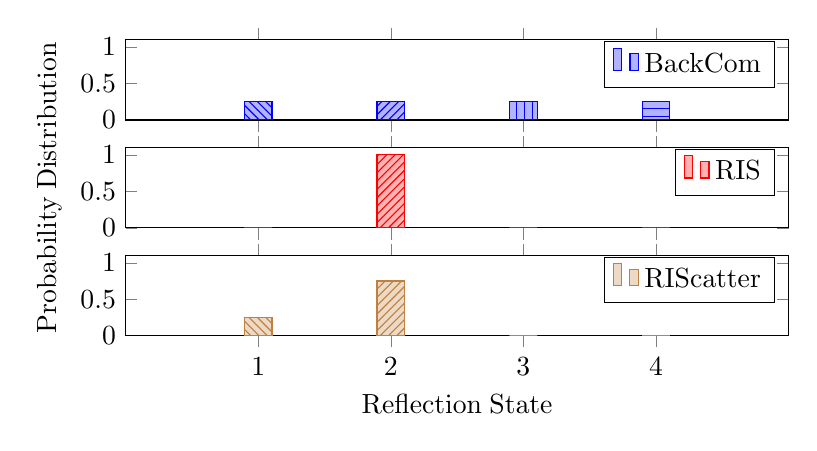
\begin{tikzpicture}
	\begin{groupplot}
		[group style={
					rows=3,
					group name=plots,
					x descriptions at=edge bottom,
					y descriptions at=edge left,
					vertical sep=10
				},
			ybar,
			xmin=0,
			xmax=4,
			xtick={1,2,3,4},
			ymin=0,
			ymax=1,
			xlabel={Reflection State},
			enlarge x limits={value=0.25,upper},
			enlarge y limits={value=0.1,upper},
			width=10cm,
			height=2.6cm,
			every axis plot/.append style={bar shift=0}
		]
		\nextgroupplot
		\addplot[blue,fill=blue!30!white] coordinates {(-1,-1)};
		\addplot[blue,fill=blue!30!white,postaction={pattern=north west lines},pattern color=.] coordinates {(1,0.25)};
		\addplot[blue,fill=blue!30!white,postaction={pattern=north east lines},pattern color=.] coordinates {(2,0.25)};
		\addplot[blue,fill=blue!30!white,postaction={pattern=vertical lines},pattern color=.] coordinates {(3,0.25)};
		\addplot[blue,fill=blue!30!white,postaction={pattern=horizontal lines},pattern color=.] coordinates {(4,0.25)};
		\legend{BackCom}
		\nextgroupplot[ylabel={Probability Distribution}]
		\addplot[red,fill=red!30!white] coordinates {(-1,-1)};
		\addplot[red,fill=red!30!white,postaction={pattern=north west lines},pattern color=.] coordinates {(1,0)};
		\addplot[red,fill=red!30!white,postaction={pattern=north east lines},pattern color=.] coordinates {(2,1)};
		\addplot[red,fill=red!30!white,postaction={pattern=vertical lines},pattern color=.] coordinates {(3,0)};
		\addplot[red,fill=red!30!white,postaction={pattern=horizontal lines},pattern color=.] coordinates {(4,0)};
		\legend{RIS}
		\nextgroupplot
		\addplot[brown,fill=brown!30!white] coordinates {(-1,-1)};
		\addplot[brown,fill=brown!30!white,postaction={pattern=north west lines},pattern color=.] coordinates {(1,0.25)};
		\addplot[brown,fill=brown!30!white,postaction={pattern=north east lines},pattern color=.] coordinates {(2,0.75)};
		\addplot[brown,fill=brown!30!white,postaction={pattern=vertical lines},pattern color=.] coordinates {(3,0)};
		\addplot[brown,fill=brown!30!white,postaction={pattern=horizontal lines},pattern color=.] coordinates {(4,0)};
		\legend{RIScatter}
	\end{groupplot}
\end{tikzpicture}

				}
				\label{fi:input_distribution}
			}
			\\
			\subfloat[Time Block]{
				\resizebox{0.8\columnwidth}{!}{
					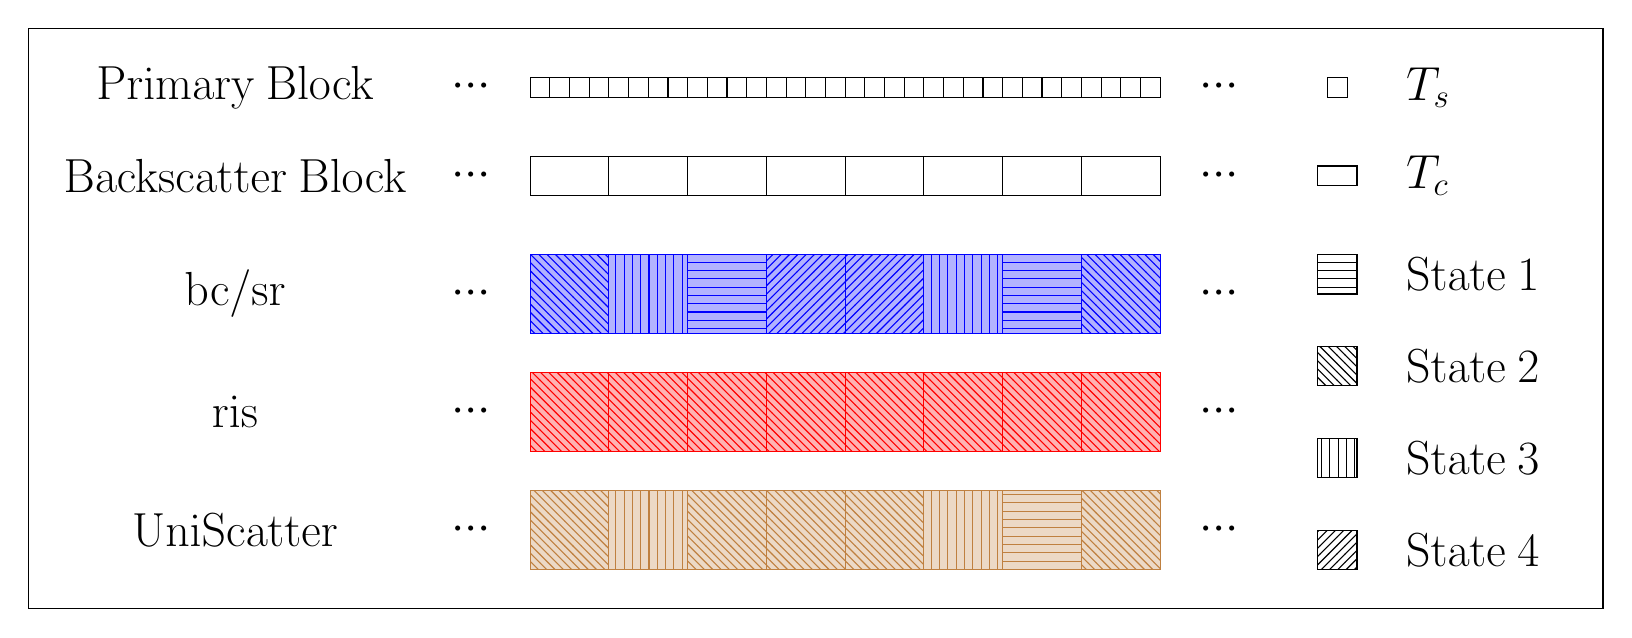
\begin{tikzpicture}
	\foreach \x in {0,...,31}{
			\draw (0.25*\x,3) rectangle ++(0.25,0.25);
		}
	\node[font=\LARGE] at (-0.75,3.125) {$\cdots$};
	\node[font=\LARGE] at (8.75,3.125) {$\cdots$};
	\node[font=\LARGE] at (-3.75,3.125) {Primary Block};
	\draw (10.125,3) rectangle ++(0.25,0.25);
	\node[font=\LARGE,right] at (11,3.125){$T_s$};

	\foreach \x in {0,...,7}{
			\draw (\x,1.75) rectangle ++(1,0.5);
		}
	\node[font=\LARGE] at (-0.75,2) {$\cdots$};
	\node[font=\LARGE] at (8.75,2) {$\cdots$};
	\node[font=\LARGE] at (-3.75,2) {Backscatter Block};
	\draw (10,1.875) rectangle ++(0.5,0.25);
	\node[font=\LARGE,right] at (11,2){$T_c$};

	\draw [blue,fill=blue!30!white,postaction={pattern=north west lines},pattern color=.](0,0) rectangle ++(1,1);
	\draw [blue,fill=blue!30!white,postaction={pattern=vertical lines},pattern color=.](1,0) rectangle ++(1,1);
	\draw [blue,fill=blue!30!white,postaction={pattern=horizontal lines},pattern color=.](2,0) rectangle ++(1,1);
	\draw [blue,fill=blue!30!white,postaction={pattern=north east lines},pattern color=.](3,0) rectangle ++(1,1);
	\draw [blue,fill=blue!30!white,postaction={pattern=north east lines},pattern color=.](4,0) rectangle ++(1,1);
	\draw [blue,fill=blue!30!white,postaction={pattern=vertical lines},pattern color=.](5,0) rectangle ++(1,1);
	\draw [blue,fill=blue!30!white,postaction={pattern=horizontal lines},pattern color=.](6,0) rectangle ++(1,1);
	\draw [blue,fill=blue!30!white,postaction={pattern=north west lines},pattern color=.](7,0) rectangle ++(1,1);
	\node[font=\LARGE] at (-0.75,0.5) {$\cdots$};
	\node[font=\LARGE] at (8.75,0.5) {$\cdots$};
	\node[font=\LARGE] at (-3.75,0.5) {\gls{bc}/\gls{sr}};

	\foreach \x in {0,...,7}{
			\draw [red,fill=red!30!white,postaction={pattern=north west lines},pattern color=.](\x,-1.5) rectangle ++(1,1);
		}
	\node[font=\LARGE] at (-0.75,-1) {$\cdots$};
	\node[font=\LARGE] at (8.75,-1) {$\cdots$};
	\node[font=\LARGE] at (-3.75,-1) {\gls{ris}};

	\draw [brown,fill=brown!30!white,postaction={pattern=north west lines},pattern color=.](0,-3) rectangle ++(1,1);
	\draw [brown,fill=brown!30!white,postaction={pattern=vertical lines},pattern color=.](1,-3) rectangle ++(1,1);
	\draw [brown,fill=brown!30!white,postaction={pattern=north west lines},pattern color=.](2,-3) rectangle ++(1,1);
	\draw [brown,fill=brown!30!white,postaction={pattern=north west lines},pattern color=.](3,-3) rectangle ++(1,1);
	\draw [brown,fill=brown!30!white,postaction={pattern=north west lines},pattern color=.](4,-3) rectangle ++(1,1);
	\draw [brown,fill=brown!30!white,postaction={pattern=vertical lines},pattern color=.](5,-3) rectangle ++(1,1);
	\draw [brown,fill=brown!30!white,postaction={pattern=horizontal lines},pattern color=.](6,-3) rectangle ++(1,1);
	\draw [brown,fill=brown!30!white,postaction={pattern=north west lines},pattern color=.](7,-3) rectangle ++(1,1);
	\node[font=\LARGE] at (-0.75,-2.5) {$\cdots$};
	\node[font=\LARGE] at (8.75,-2.5) {$\cdots$};
	\node[font=\LARGE] at (-3.75,-2.5) {UniScatter};

	\draw [pattern=horizontal lines](10,0.5) rectangle ++(0.5,0.5);
	\draw [pattern=north west lines](10,-2/3) rectangle ++(0.5,0.5);
	\draw [pattern=vertical lines](10,-11/6) rectangle ++(0.5,0.5);
	\draw [pattern=north east lines](10,-3) rectangle ++(0.5,0.5);
	\node[font=\LARGE,right] at (11,0.75){State 1};
	\node[font=\LARGE,right] at (11,-5/12){State 2};
	\node[font=\LARGE,right] at (11,-19/12){State 3};
	\node[font=\LARGE,right] at (11,-2.75){State 4};
	\draw (-6.375,-3.5) rectangle ++(20, 7.375);
\end{tikzpicture}

				}
				\label{fi:time_block}
			}
			\caption{
				Input probability distribution and time block structure of \gls{bc}, \gls{sr}, \gls{ris}, and RIScatter.
				$T_s$ and $T_c$ respectively denote the primary and backscatter symbol period.
				Within channel coherence time, RIScatter nodes semi-randomly select reflection state for each backscatter symbol block under the guidance of input probability distribution.
			}
			\label{fi:riscatter_distribution}
		\end{figure}
		As illustrated in Fig. \ref{fi:riscatter_distribution}, instead of always using fully random or deterministic reflection pattern over time, each RIScatter node can \emph{flexibly adjust} its input distribution to balance information encoding and channel reconfiguration.
		That is, it semi-randomly select the reflection state per backscatter symbol block under the guidance of input probability $P(\Gamma_m)$ for state $m$.
		Such an adaptive backscatter channel coding coincides with \gls{ris} when primary link is absolutely prioritized, and outperforms the conventional equiprobable line-coded \gls{bc}/\gls{sr} when backscatter link is absolutely prioritized.
		Besides, the dispersed characteristics of RIScatter nodes (and legacy users) avoids the development optimization and allows uniformly good performance for both links.

		As shown in Fig. \subref*{fi:block_diagram}, RIScatter nodes can be implemented over readily available passive backscatter devices with energy harvester and information decoder.
		Its equivalent circuit and scatter model are presented in Fig. \subref*{fi:equivalent_circuit} and \subref*{fi:scatter_model}.
		When activated by primary transmitter, each node harvests a proportion of the impinging wave for its own operation, decode the embedded coordination information for input distribution control, then applies a potentially random phase shift on the reradiated signal due to backscatter modulation.
		Energy harvesting and information decoding at passive RIScatter nodes can be realized using conventional power-splitting or time-sharing \gls{swipt} protocols \cite{Clerckx2019} or integrated energy-information receiver with pulse position modulated signal \cite{Kim2021a}.
		Besides, relevant \gls{csi} can be acquired using either traditional sequential methods \cite{Bharadia2015,Yang2015b,Guo2019g} or the state-of-the-art parallel approach \cite{Jin2021a}.
		In the following context, we assume perfect primary-total-backscatter coordination and perfect channel estimation for all links.
		\begin{figure*}[!t]
			\centering
			\subfloat[Block Diagram]{
				\resizebox{0.32\linewidth}{!}{
					\makeatletter
\tikzset{
	block/.style={draw,rectangle,align=center},
	from/.style args={#1 to #2}{
			above right={0cm of #1},
			/utils/exec=\pgfpointdiff
			{\tikz@scan@one@point\pgfutil@firstofone(#1)\relax}
			{\tikz@scan@one@point\pgfutil@firstofone(#2)\relax},
			minimum width/.expanded=\the\pgf@x,
			minimum height/.expanded=\the\pgf@y
		}
}
\makeatother

\begin{circuitikz}[transform shape]
	\tikzstyle{every node}=[font=\small]
	\coordinate (O) at (0,0);
	\node[block,from={O to $(O) + (6.375,3)$}](T){};
	\draw (0,1.5)
	to[short] ++(-0.875,0)
	to[short] ++(0,0.5) node[bareantenna](A){Bx};
	\draw (0,1.5)
	to[short,-*] ++(0.25,0) coordinate(J);
	\draw (J)
	to[short] ++(0,1)
	to[short] ++(0.5,0) coordinate(J1);
	\node[block,from={$(J1) + (0,-0.25)$ to $(J1) + (2.5,0.25)$}](R){Rectifier};
	\draw (J)
	to[short] ++(0.5,0) coordinate(J2);
	\node[block,from={$(J2) + (0,-0.25)$ to $(J2) + (2.5,0.25)$}](D){Demodulator};
	\draw (J)
	to[short] ++(0,-1)
	to[short] ++(0.5,0) coordinate(J3);
	\node[block,from={$(J3) + (0,-0.25)$ to $(J3) + (2.5,0.25)$}](M){Modulator};
	\draw[dashed,-{Latex[length=2mm]}] (R.east) -- ++(0.75,0);
	\draw[-{Latex[length=2mm]}] (D.east) -- ++(0.75,0);
	\draw[{Latex[length=2mm]}-] (M.east) -- ++(0.75,0);
	\node[block,from={$(R.east) + (0.75,-0.25)$ to $(R.east) + (2.875,0.25)$}](P){Power Buffer};
	\node[block,from={$(M.east) + (0.75,-0.25)$ to $(D.east) + (2.875,0.25)$}](S){Digital\\Section};
	\draw[dashed,-{Latex[length=2mm]}] (P.south) to (S.north);
	\coordinate (F1) at ($(P.south)!0.5!(S.north)$);
	\coordinate (F2) at ($(D.east)!0.5!(S.west)$);
	\coordinate (F3) at ($(D.south)!0.5!(M.north)$);
	\draw[dashed] (F1) to (F1-|D.north);
	\draw[dashed,-{Latex[length=2mm]}] (F1-|D.north) to (D.north);
	\draw[dashed] (F1-|F2) to (F2|-F3) to (M|-F3);
	\draw[dashed,-{Latex[length=2mm]}] (M|-F3) to (M.north);
\end{circuitikz}

				}
				\label{fi:block_diagram}
			}
			\subfloat[Equivalent Circuit]{
				\resizebox{0.37\linewidth}{!}{
					\begin{circuitikz}[transform shape]
	\tikzstyle{every node}=[font=\Large]
	\draw (0,0) coordinate(O)
	to [sV,l=$V_0$] ++(0,1.5)
	to [L,l=$X_{\mathrm{A}}$] ++(0,1.5)
	to [R=$R_{\mathrm{A}}$,-*] ++(3,0) coordinate(AM)
	to [sI,l_=$I_0$,-*] ++(0,-3)
	to [short] (O);
	\draw (AM)
	to [short] ++(0.5,0)
	to [L,l=$X_m$,-*] ++(3,0) coordinate(M)
	to [R=$R_m^{\mathrm{S}}$] ++(3,0) coordinate(MH);
	\draw (M)
	to [R=$R_m^{\mathrm{P}}$,-*] ++(0,-3);
	\draw (MH)
	to [D,-*] ++(1.5,0) coordinate(H)
	to [C=$X_{\mathrm{H}}$,-*] ++(0,-3);
	\draw (H)
	to [short] ++(1.5,0)
	to [R=$R_{\mathrm{H}}$] ++(0,-3)
	to [short] (O);

	\draw [dashed] (-1.125,-0.5) rectangle (3.5,4);
	\draw [dashed] (4,-0.5) rectangle (9,4);
	\draw [dashed] (9.5,-0.5) rectangle (13.5,4);

	\draw (1.125,4.25) node[]{Antenna};
	\draw (6.5,4.25) node[]{Modulator};
	\draw (11.5,4.25) node[]{Harvester \& Chip};

	\draw (3.375,2.675) to [short] (3.375,3.175) to [short] (3.25,3.175) to [short,i_=$Z_{\mathrm{A}}$] (3.125,3.175);
	\draw (4.125,-0.125) to [short] (4.125,0.375) to [short] (4.25,0.375) to [short,i=$Z_m$] (4.375,0.375);
	\draw (9.625,-0.125) to [short] (9.625,0.375) to [short] (9.75,0.375) to [short,i=$Z_{\mathrm{H}}$] (9.875,0.375);
\end{circuitikz}

				}
				\label{fi:equivalent_circuit}
			}
			\subfloat[Scatter Model]{
				\resizebox{0.28\linewidth}{!}{
					\begin{circuitikz}[transform shape]
	\tikzstyle{every node}=[font=\large]
	\ctikzset{multipoles/rotary/arrow=both}
	\draw (0,0) node[bareantenna](bareantenna){};
	\draw (bareantenna.west) ++(-1,0) node[waves](WI){};
	\draw (WI.north east) ++(0.25,0) node{$\vec{E}_{\text{I}}$};
	\draw (WI.south east) ++(0.25,0) node{$\vec{H}_{\text{I}}$};
	\draw (bareantenna.east) ++(0.5,0) node[waves](WR){};
	\draw (WR.north east) ++(0.35,0) node{$\vec{E}_m$};
	\draw (WR.south east) ++(0.35,0) node{$\vec{H}_m$};
	\draw (bareantenna) to ++(0,-1.1) to [generic,l=$Z_{\text{A}}$,/tikz/circuitikz/bipoles/length=0.75cm] ++(2.3,0) node[rotary switch=4 in 90 wiper 30,anchor=ext center,rotate=0](SW){};
	\draw (SW.cout 1) to ++(0.625,+0.5) to [generic,/tikz/circuitikz/bipoles/length=0.75cm] ++(2.2,0) coordinate(E1);
	\draw (SW.cout 2) node[above right]{$m$} to [generic,l=$Z_m$,/tikz/circuitikz/bipoles/length=0.75cm] ++(2.2,0) coordinate(E2);
	\draw (SW.cout 3) to [generic,/tikz/circuitikz/bipoles/length=0.75cm] ++(2.2,0) coordinate(E3);
	\draw (SW.cout 4) to ++(0.625,-0.5) to [generic,/tikz/circuitikz/bipoles/length=0.75cm] ++(2.2,0) coordinate(E4);
	\draw (E1) to[short,-*] (E2);
	\draw (E2) to[short,-*] (E3);
	\draw (E3) to[short] (E4);
	\draw (E2) to[short] ++(0.2,0) node[ground,rotate=90]{};
\end{circuitikz}

				}
				\label{fi:scatter_model}
			}
			\caption{
			Block diagram, equivalent circuit, and scatter model of a RIScatter node.
			The solid and dashed vectors represent signal and energy flows.
			The scattering antenna behaves as a constant power source, where the voltage $V_0$ and current $I_0$ are introduced by incident electric field $\vec{E}_{\mathrm{I}}$ and magnetic field $\vec{H}_{\mathrm{I}}$ \cite{Huang2021}.
			}
			\label{fi:riscatter_node}
		\end{figure*}
	\end{subsection}

	\begin{subsection}{RIScatter Receiver}
		Since each passive RIScatter node directly modulates its own message over the legacy signal, it involves a \emph{double modulation} where the primary and backscatter symbols are superimposed by \emph{multiplication coding} instead of superposition coding.
		Besides, the backscatter symbol period is typically longer than primary due to the load switching speed constraint.
		Those facts imply \emph{backscatter detection} under primary uncertainty can be viewed as part of \emph{primary channel training}.
		Hence, we propose a practical RIScatter receiver that semi-coherently decodes RIScatter nodes from the received energy per backscatter block, re-encodes for their reflection patterns, retrieves primary equivalent channel as if dynamic passive beamforming, then coherently decodes the primary link under the enhanced multipath.
		\begin{figure}[!t]
			\centering
			\resizebox{0.9\columnwidth}{!}{
				\definecolor{color1}{HTML}{0072BD}
\definecolor{color2}{HTML}{D95319}
\definecolor{color3}{HTML}{EDB120}
\definecolor{color4}{HTML}{7E2F8E}

\begin{tikzpicture}
	\begin{axis}[
			clip mode=individual,
			height=5cm,
			width=9cm,
			xlabel = $z$,
			ylabel = {Probability Density},
			font=\scriptsize,
			no markers,
			xmin=0,
			ymin=0,
			xmax=70,
			xtick={0,12.78,20.28,29.62,70},
			xticklabels={$t_0$,$t_1$,$t_2$,$t_3$,$t_4$},
			yticklabels=\empty,
			samples = 200
		]

		\addplot+[very thick,solid,color1] gnuplot[raw gnuplot] {%
				isint(x) = (int(x)==x);
				gmm(x,rho,lambda)=rho<=0||lambda<=0?1/0:  x<0?0.0:x==0?(rho>1?0.0:rho==1?real(lambda):1/0):  exp(rho*log(lambda)+(rho-1.0)*log(x)-lgamma(rho)-lambda*x);
				set xrange [0:80];
				set yrange [0:1];
				samples=200;
				plot gmm(x,10,1)};
		\addlegendentryexpanded{$f(z \mid \mathcal{H}_1)$}

		\addplot+[very thick,dashed,color2] gnuplot[raw gnuplot] {%
				isint(x) = (int(x)==x);
				gmm(x,rho,lambda)=rho<=0||lambda<=0?1/0:  x<0?0.0:x==0?(rho>1?0.0:rho==1?real(lambda):1/0):  exp(rho*log(lambda)+(rho-1.0)*log(x)-lgamma(rho)-lambda*x);
				set xrange [0:80];
				set yrange [0:1];
				samples=200;
				plot gmm(x,10,0.6)};
		\addlegendentryexpanded{$f(z \mid \mathcal{H}_2)$}

		\addplot+[very thick,dotted,color3] gnuplot[raw gnuplot] {%
				isint(x) = (int(x)==x);
				gmm(x,rho,lambda)=rho<=0||lambda<=0?1/0:  x<0?0.0:x==0?(rho>1?0.0:rho==1?real(lambda):1/0):  exp(rho*log(lambda)+(rho-1.0)*log(x)-lgamma(rho)-lambda*x);
				set xrange [0:80];
				set yrange [0:1];
				samples=200;
				plot gmm(x,10,0.4)};
		\addlegendentryexpanded{$f(z \mid \mathcal{H}_3)$}

		\addplot+[very thick,dashdotted,color4] gnuplot[raw gnuplot] {%
				isint(x) = (int(x)==x);
				gmm(x,rho,lambda)=rho<=0||lambda<=0?1/0:  x<0?0.0:x==0?(rho>1?0.0:rho==1?real(lambda):1/0):  exp(rho*log(lambda)+(rho-1.0)*log(x)-lgamma(rho)-lambda*x);
				set xrange [0:80];
				set yrange [0:1];
				samples=200;
				plot gmm(x,10,0.28)};
		\addlegendentryexpanded{$f(z \mid \mathcal{H}_4)$}
		\draw[latex-latex] (0,0) -- (12.78,0) node[above,midway,yshift=-2]{$\mathcal{R}_1$};
		\draw[latex-latex] (12.78,0) -- (20.28,0) node[above,midway,yshift=-2]{$\mathcal{R}_2$};
		\draw[latex-latex] (20.28,0) -- (29.62,0) node[above,midway,yshift=-2]{$\mathcal{R}_3$};
		\draw[latex-latex] (29.62,0) -- (70,0) node[above,midway,yshift=-2]{$\mathcal{R}_4$};
	\end{axis}
\end{tikzpicture}

			}
			\caption{
				\gls{pdf} of total received energy per backscatter block, conditioned on different input state hypotheses.
				$t$ and $\mathcal{R}$ denote the energy decision thresholds and regions, respectively.
			}
			\label{fi:energy_distribution}
		\end{figure}
		As illustrated in Fig. \ref{fi:energy_distribution}, the total received energy per backscatter block is a random variable that follows different distributions conditioned on different input state hypotheses.
		Compared with conventional joint \gls{ml} and \gls{sic} from stronger primary link to weaker backscatter links, RIScatter receiver not only preserves the benefits of backscatter modulation and passive beamforming, but also enjoys much lower computational and operational complexities.
	\end{subsection}

	\begin{subsection}{System Model}
		\begin{figure}[!t]
			\centering
			\def\svgwidth{0.8\columnwidth}
			\footnotesize{
				\import{assets/illustration/}{riscatter_network.pdf_tex}
			}
			\caption{A single-user multi-node RIScatter system.}
			\label{fi:riscatter_network}
		\end{figure}
		To demonstrate the advantages of RIScatter, we consider a single-user multi-node \gls{miso} RIScatter system as shown in Fig. \ref{fi:riscatter_network}.
		In the primary active point-to-point system, a $Q$-antenna \gls{ap} transmits to a single-antenna user assisted by $K$ nearby single-antenna RIScatter nodes with $M$ reflection states.
		In the secondary backscatter \gls{mac} system, the \gls{ap} serves as the carrier emitter, the distributed RIScatter nodes modulate information over reradiated \gls{rf} signals, and the user decodes their messages.
		For simplicity, we consider a quasi-static block fading model where channels remain constant within coherence block and vary independently between consecutive blocks.
		Due to the physical constraints of load switching speed, we assume the backscatter over primary symbol period ratio is an integer $N \gg 1$.
		We also omit the signal reflected by two or more times and ignore the propagation time difference of different paths.

		Denote the \gls{ap}-user direct channel as $\boldsymbol{h}_{\mathrm{D}}^H \in \mathbb{C}^{1 \times Q}$, the \gls{ap}-node $k \in \mathcal{K} \triangleq \{1,\ldots,K\}$ forward channel as $\boldsymbol{h}_{\mathrm{F},k}^H \in \mathbb{C}^{1 \times Q}$, the node $k$-user backward channel as $h_{\mathrm{B},k}$, and the cascaded channel via tag $k$ as $\boldsymbol{h}_{\mathrm{C},k}^H \triangleq h_{\mathrm{B},k} \boldsymbol{h}_{\mathrm{F},k}^H \in \mathbb{C}^{1 \times Q}$.
		Let $x_{\mathcal{K}} \triangleq (x_1,\ldots,x_K)$ be the backscatter symbol tuple of all RIScatter nodes.
		Without loss of generality, we consider one specific backscatter block (i.e., $N$ primary blocks) in the following context.
		Due to double modulation, the primary equivalent channel is a function of \emph{coded} backscatter symbols\footnote{Expression \eqref{eq:equivalent_channel_bc} is often used in \gls{bc} literatures while expression \eqref{eq:equivalent_channel_ris} is commonly observed in \gls{ris} literatures.}
		% \begin{equation}
		% 	\boldsymbol{h}_{\mathrm{E}}^H(x_{\mathcal{K}}) \overset{\text{(a)}}{=} \boldsymbol{h}_{\mathrm{D}}^H + \sum_{k} \alpha_k \boldsymbol{h}_{\mathrm{C},k}^H x_k \overset{\text{(b)}}{=} \boldsymbol{h}_{\mathrm{D}}^H + \boldsymbol{x}^H \mathrm{diag}(\boldsymbol{\alpha}) \boldsymbol{H}_{\mathrm{C}},
		% 	\label{eq:equivalent_channel}
		% \end{equation}
		\begin{subequations}
			\begin{align}
				\boldsymbol{h}_{\mathrm{E}}^H(x_{\mathcal{K}})
				 & \triangleq \boldsymbol{h}_{\mathrm{D}}^H + \sum_{k} \alpha_k \boldsymbol{h}_{\mathrm{C},k}^H x_k \label{eq:equivalent_channel_bc}                    \\
				 & = \boldsymbol{h}_{\mathrm{D}}^H + \boldsymbol{x}^H \mathrm{diag}(\boldsymbol{\alpha}) \boldsymbol{H}_{\mathrm{C}}, \label{eq:equivalent_channel_ris}
			\end{align}
			\label{eq:equivalent_channel}
		\end{subequations}
		where $\alpha_k \in \mathbb{I}$ is the amplitude scattering ratio of RIScatter node $k$, $x_k \in \mathcal{X} \triangleq \{c_1,\ldots,c_M\}$ is the \emph{coded} backscatter symbol of node $k$, $\boldsymbol{\alpha} \triangleq [\alpha_1,\ldots,\alpha_K]^T \in \mathbb{I}^{K}$, $\boldsymbol{x} \triangleq [x_1,\ldots,x_K]^H \in \mathcal{X}^{K}$, and $\boldsymbol{H}_{\mathrm{C}} \triangleq [\boldsymbol{h}_{\mathrm{C},1},\ldots,\boldsymbol{h}_{\mathrm{C},K}]^H \in \mathbb{C}^{K \times Q}$.
		The signal received by the user at primary block $n \in \mathcal{N} \triangleq \{1,\ldots,N\}$ is
		\begin{equation}
			y[n] = \boldsymbol{h}_{\mathrm{E}}^H(x_{\mathcal{K}}) \boldsymbol{w} s[n] + v[n],
			\label{eq:receive_signal}
		\end{equation}
		where $s \sim \mathcal{CN}(0,1)$ is the primary symbol, $v \sim \mathcal{CN}(0,\sigma_v^2)$ is the \gls{awgn}, and $\boldsymbol{w} \in \mathbb{C}^{Q}$ is the active beamforming vector subject to average transmit power constraint $\lVert \boldsymbol{w} \rVert^2 \le P$.
		Denote $m_k \in \mathcal{M} \triangleq \{1,\ldots,M\}$ as the reflection state index of node $k$, and $m_{\mathcal{K}} \triangleq (m_1,\ldots,m_K)$ as the state index tuple of all nodes.
		Conditioned on backscatter index tuple $m_{\mathcal{K}}$, the received signal at each primary block follows \gls{cscg} distribution $\mathcal{CN}(0,\sigma_{m_{\mathcal{K}}}^2)$, where
		\begin{equation}
			\sigma_{m_{\mathcal{K}}}^2 = \lvert \boldsymbol{h}_{\mathrm{E}}^H(x_{m_{\mathcal{K}}}) \boldsymbol{w} \rvert^2 + \sigma_v^2
			\label{eq:receive_variance}
		\end{equation}
		is the received variance and $x_{m_\mathcal{K}}$ is the backscatter symbol tuple associated with $m_{\mathcal{K}}$.
		For node $k$, let $x_{m_k}$ be the backscatter symbol associated with index $m_k$.%
		\footnote{
			Please note $x_k$ and $x_{\mathcal{K}}$ are random variable and tuple, while $x_{m_k}$ and $x_{m_{\mathcal{K}}}$ are their instances of index $m_k$ and $m_{\mathcal{K}}$.
		}
		Besides, we define the total received energy per backscatter block as $z=\sum_{n \in \mathcal{N}} \bigl\lvert y[n] \bigr\rvert^2$.
		Since $z$ is the sum of $N$ \gls{iid} exponential variables, its \gls{pdf} conditioned on $m_{\mathcal{K}}$ follows Gamma distribution
		\begin{equation}
			f(z|\mathcal{H}_{m_{\mathcal{K}}}) = \frac{z^{N-1} \exp(-z/\sigma_{m_{\mathcal{K}}}^2)}{\sigma_{m_{\mathcal{K}}}^{2N} (N-1)!},
			\label{eq:energy_distribution}
		\end{equation}
		where $\mathcal{H}_{m_{\mathcal{K}}}$ denotes hypothesis $m_{\mathcal{K}}$.
		As illustrated in Fig. \ref{fi:energy_distribution}, the RIScatter receiver divides the received energy space into disjoint decision regions associated with those hypotheses.
		For example, if the total received energy during a backscatter block falls within region $\mathcal{R}_{m_{\mathcal{K}}}$, then the detector output would be $x_{m_{\mathcal{K}}}$.
		\begin{remark}
			Interestingly, the capacity-achieving decision design for \gls{dmtc} remains under-investigated, and some attempts were made for a single source with binary inputs \cite{Qian2019b,Nguyen2021b}.
			For non-binary inputs with arbitrary distribution, the optimal decision region for each letter can be non-convex (i.e., with non-adjacent partitions) and the optimal number of thresholds is still unknown \cite{Nguyen2018,Nguyen2021}.
		\end{remark}
		Like most existing literatures, we limit the scope of this paper to convex decision regions and consider sequential decision thresholds design therein.
		For the ease of notations, we define a general bijective function from backscatter index tuple $m_{\mathcal{K}}$ to integer $l \in \mathcal{L} \triangleq \{1,\ldots,L \triangleq M^K\}$, where $\{\sigma_l^2\}_{l \in \mathcal{L}}$ are sorted in an ascending order.
		Both notations are used interchangeably in the following context.
		As such, the convex decision region of backscatter tuple $l$ can be written as
		\begin{equation}
			\mathcal{R}_{l} \triangleq [t_{l-1},t_l), \quad 0 \le t_{l-1} \le t_l.
		\end{equation}
		Once the decision threshold vector $\boldsymbol{t} \triangleq [t_0,\ldots,t_L]^T \in \mathbb{R}_+^{(L+1)}$ is determined, we can formulate a \gls{dmtmac} with transition probability from input $x_{m_{\mathcal{K}}}$ to output $\hat{x}_{m_{\mathcal{K}}'}$
		\begin{equation}
			P(\hat{x}_{m_{\mathcal{K}}'}|x_{m_{\mathcal{K}}}) = \int_{\mathcal{R}_{m_{\mathcal{K}}'}} f(z|\mathcal{H}_{m_{\mathcal{K}}}) \, d z,
			\label{eq:dmtmac}
		\end{equation}
		then perform backscatter channel coding on top of it.
		\label{se:system_model}
	\end{subsection}

	\begin{subsection}{Information Theory}
		Denote the input probability distribution vector of node $k$ as $\boldsymbol{p}_k \triangleq [P_k(c_1),\ldots,P_k(c_M)]^T \in \mathbb{I}^{M}$, and the probability of state $m_k$ as $P_k(x_{m_k})$.
		With independent encoding at all nodes, the probability of backscatter symbol tuple $x_{m_{\mathcal{K}}}$ is
		\begin{equation}
			P_{\mathcal{K}}(x_{m_{\mathcal{K}}}) = \prod_{k \in \mathcal{K}} P_k(x_{m_k}).
			\label{eq:equivalent_distribution}
		\end{equation}

		Similar to \cite{Rezaeian2004}, we define the backscatter information function between input symbol tuple instance $x_{m_{\mathcal{K}}}$ and output symbol tuple variable $\hat{x}_{\mathcal{K}}$ as
		\begin{equation}
			I_{\mathrm{B}}(x_{m_{\mathcal{K}}};\hat{x}_{\mathcal{K}}) \triangleq \sum_{m_{\mathcal{K}}'} P(\hat{x}_{m_{\mathcal{K}}'}|x_{m_{\mathcal{K}}}) \log \frac{P(\hat{x}_{m_{\mathcal{K}}'}|x_{m_{\mathcal{K}}})}{P_{\mathcal{K}}(\hat{x}_{m_{\mathcal{K}}'})},
			\label{eq:backscatter_information_function}
		\end{equation}
		where $P_{\mathcal{K}}(\hat{x}_{m_{\mathcal{K}}'}) = \sum_{m_{\mathcal{K}}} P_{\mathcal{K}}(x_{m_{\mathcal{K}}}) P(\hat{x}_{m_{\mathcal{K}}'}|x_{m_{\mathcal{K}}})$ is the probability of channel output tuple $\hat{x}_{m_{\mathcal{K}}'}$.
		We also define the backscatter marginal information of letter $x_{m_k}$ of node $k$ as
		\begin{equation}
			I_{\mathrm{B},k}(x_{m_k};\hat{x}_{\mathcal{K}}) \triangleq \sum_{m_{\mathcal{K} \setminus \{k\}}} P_{\mathcal{K} \setminus \{k\}}(x_{m_{\mathcal{K} \setminus \{k\}}}) I_{\mathrm{B}}(x_{m_{\mathcal{K}}};\hat{x}_{\mathcal{K}}),
			\label{eq:backscatter_marginal_information}
		\end{equation}
		where $P_{\mathcal{K} \setminus \{k\}}(x_{m_{\mathcal{K} \setminus \{k\}}}) = \prod_{q \in \mathcal{K} \setminus \{k\}} P_{q}(x_{m_{q}})$.
		The backscatter mutual information can be written as
		\begin{equation}
			I_{\mathrm{B}}(x_{\mathcal{K}};\hat{x}_{\mathcal{K}}) = \sum_{m_{\mathcal{K}}} P_{\mathcal{K}}(x_{m_{\mathcal{K}}}) I_{\mathrm{B}}(x_{m_{\mathcal{K}}};\hat{x}_{\mathcal{K}}).
			\label{eq:backscatter_mutual_information}
		\end{equation}
		Once backscatter messages of all nodes are successfully decoded, we can re-code for backscatter symbol tuple $x_{\mathcal{K}}$, recover their reflection patterns by \eqref{eq:backscatter_modulation}, and retrieve the primary equivalent channel by \eqref{eq:equivalent_channel}.
		Moreover, we define the primary information function conditioned on backscatter symbol tuple $x_{m_{\mathcal{K}}}$ as
		\begin{equation}
			I_{\mathrm{P}}(s;y|x_{m_{\mathcal{K}}}) \triangleq \log \Bigl(1 + \frac{\lvert \boldsymbol{h}_{\mathrm{E}}^H(x_{m_{\mathcal{K}}}) \boldsymbol{w} \rvert^2}{\sigma_v^2}\Bigr),
			\label{eq:primary_information_function}
		\end{equation}
		the primary marginal information conditioned on letter $x_{m_k}$ of node $k$ as
		\begin{equation}
			I_{\mathrm{P},k}(s;y|x_{m_k}) \triangleq \sum_{m_{\mathcal{K} \setminus \{k\}}} P_{\mathcal{K} \setminus \{k\}}(x_{m_{\mathcal{K} \setminus \{k\}}}) I_{\mathrm{P}}(s;y|x_{m_{\mathcal{K}}}),
			\label{eq:primary_marginal_information}
		\end{equation}
		and the primary ergodic mutual information as
		\begin{equation}
			I_{\mathrm{P}}(s;y|x_{\mathcal{K}}) = \sum_{m_{\mathcal{K}}} P_{\mathcal{K}}(x_{m_{\mathcal{K}}}) I_{\mathrm{P}}(s;y|x_{m_{\mathcal{K}}}).
			\label{eq:primary_mutual_information}
		\end{equation}

		With a slight abuse of notation, we define the corresponding weighted sum information function, marginal information, and mutual information respectively as
		\begin{align}
			I(x_{m_{\mathcal{K}}})
			 & \triangleq \rho I_{\mathrm{P}}(s;y|x_{m_{\mathcal{K}}}) + (1 - \rho) I_{\mathrm{B}}(x_{m_{\mathcal{K}}};\hat{x}_{\mathcal{K}}),\label{eq:weighted_sum_information_function} \\
			I_k(x_{m_k})
			 & \triangleq \rho I_{\mathrm{P},k}(s;y|x_{m_k}) + (1 - \rho) I_{\mathrm{B},k}(x_{m_k};\hat{x}_{\mathcal{K}}),\label{eq:weighted_sum_marginal_information}                     \\
			I(x_{\mathcal{K}})
			 & \triangleq \rho I_{\mathrm{P}}(s;y|x_{\mathcal{K}}) + (1 - \rho) I_{\mathrm{B}}(x_{\mathcal{K}};\hat{x}_{\mathcal{K}}),\label{eq:weighted_sum_mutual_information}
		\end{align}
		where $\rho \in \mathbb{I}$ is the relative priority of the primary link.
		\label{se:information_theory}
	\end{subsection}
	\label{se:riscatter}
\end{section}

\begin{section}{Rate-Region Characterization}
	We notice the primary ergodic mutual information \eqref{eq:primary_mutual_information} relates to input distribution and active beamforming, while the total backscatter mutual information \eqref{eq:backscatter_mutual_information} depends explicitly on input distribution and implicitly on active beamforming and decision thresholds via backscatter \gls{dmtmac} \eqref{eq:dmtmac}.
	To characterize the achievable primary-total-backscatter rate region of the proposed RIScatter system, we aim to maximize the weighted sum mutual information with respect to input distribution $\{\boldsymbol{p}_k\}_{k \in \mathcal{K}}$, active beamforming $\boldsymbol{w}$, and decision thresholds $\boldsymbol{t}$ as
	\begin{maxi!}
		{\scriptstyle{\{\boldsymbol{p}_k\}_{k \in \mathcal{K}},\boldsymbol{w},\boldsymbol{t}}}{I(x_{\mathcal{K}})}{\label{op:weighted_sum_rate}}{\label{ob:weighted_sum_rate}}
		\addConstraint{\boldsymbol{1}^T \boldsymbol{p}_k}{=1,}{\quad \forall k}{\label{co:sum_probability}}
		\addConstraint{\boldsymbol{p}_k}{\ge \boldsymbol{0},}{\quad \forall k}{\label{co:nonnegative_probability}}
		\addConstraint{\lVert \boldsymbol{w} \rVert^2}{\le P}{\label{co:transmit_power}}
		\addConstraint{t_{l-1}}{\le t_l,}{\quad \forall l}{\label{co:sequential_threshold}}
		\addConstraint{\boldsymbol{t}}{\ge \boldsymbol{0}.}{\label{co:nonnegative_threshold}}
	\end{maxi!}

	Problem \eqref{op:weighted_sum_rate} introduces adaptive backscatter channel coding over conventional \gls{bc}/\gls{sr} designs.
	% Problem \eqref{op:weighted_sum_rate} generalizes conventional \gls{bc}/\gls{sr} by allowing adaptive backscatter channel coding.
	On the other hand, it also generalizes the discrete \gls{ris} phase shift selection problem by relaxing the feasible domain from the vertices of $M$-dimensional probability simplex to the simplex itself.
	Since problem \eqref{op:weighted_sum_rate} is highly non-convex, we propose a \gls{bcd} algorithm that iteratively updates $\{\boldsymbol{p}_k\}_{k \in \mathcal{K}}$, $\boldsymbol{w}$ and $\boldsymbol{t}$ until convergence.

	\begin{subsection}{Input Distribution}
		For any given $\boldsymbol{w}$ and $\boldsymbol{t}$, we can construct the equivalent \gls{dmtmac} by \eqref{eq:dmtmac} and simplify \eqref{op:weighted_sum_rate} to
		\begin{maxi!}
			{\scriptstyle{\{\boldsymbol{p}_k\}_{k \in \mathcal{K}}}}{I(x_{\mathcal{K}})}{\label{op:input_distribution}}{}
			\addConstraint{\eqref{co:sum_probability},\eqref{co:nonnegative_probability},}
		\end{maxi!}
		which involves the coupled term $\prod_{k \in \mathcal{K}} P_k(x_{m_k})$ and is non-convex when $K > 1$.
		Following \cite{Rezaeian2004}, we first recast \gls{kkt} conditions of problem \eqref{op:input_distribution} to their equivalent forms, then propose a numerical method that guarantees those conditions on convergence of sequences.
		% ? Next, we propose a numerical method that evaluate the \gls{kkt} input distribution by limit of sequences.
		\begin{remark}
			As demonstrated in \cite{Buhler2011}, \gls{kkt} conditions are generally necessary but insufficient for total rate maximization problems.
			Although \gls{kkt} solutions to problem \eqref{op:input_distribution} may end up being saddle points, we will later show by simulation their average performance can be reasonably close to optimal for a moderate $K$.
			\label{re:input_kkt_distribution}
		\end{remark}
		\begin{proposition}
			The \gls{kkt} optimality conditions for problem \eqref{op:input_distribution} are equivalent to, $\forall k,m_k$,
			\begin{subequations}
				\label{eq:input_kkt_condition}
				\begin{alignat}{2}
					I_k^\star(x_{m_k}) & = I^\star(x_{\mathcal{K}}), \quad   &  & P_k^\star(x_{m_k}) > 0,\label{eq:probable_states} \\
					I_k^\star(x_{m_k}) & \le I^\star(x_{\mathcal{K}}), \quad &  & P_k^\star(x_{m_k}) = 0.\label{eq:dropped_states}
				\end{alignat}
			\end{subequations}
			\label{pr:input_kkt_condition}
		\end{proposition}

		\begin{proof}
			Please refer to Appendix \ref{ap:input_kkt_condition}.
			\label{pf:input_kkt_condition}
		\end{proof}

		For each node, \eqref{eq:probable_states} suggests each probable state should produce the same marginal information (averaged over all states of other nodes), while \eqref{eq:dropped_states} suggests any state with potentially less marginal information should not be used.
		\begin{proposition}
			For any strictly positive initializer $\{\boldsymbol{p}_k^{(0)}\}_{k \in \mathcal{K}}$, the \gls{kkt} input probability of node $k$ at state $m_k$ is given by the converging point of the sequence
			\begin{equation}
				P_k^{(r+1)}(x_{m_k}) = \frac{P_k^{(r)}(x_{m_k}) \exp \Bigl( \frac{\rho}{1 - \rho} I_k^{(r)}(x_{m_k}) \Bigr)}{\sum_{m_k'} P_k^{(r)}(x_{m_k'}) \exp \Bigl( \frac{\rho}{1 - \rho} I_k^{(r)}(x_{m_k'}) \Bigr)},
				\label{eq:input_kkt_solution}
			\end{equation}
			where $r$ is the iteration index.
			\label{pr:input_kkt_solution}
		\end{proposition}
		\begin{proof}
			Please refer to Appendix \ref{ap:input_kkt_solution}.
			\label{pf:input_kkt_solution}
		\end{proof}

		For \eqref{eq:input_kkt_solution} at iteration $r+1$, the input distribution of node $k$ is updated over $\bigl\{\{\boldsymbol{p}_q^{(r+1)}\}_{q=1}^{k-1},\{\boldsymbol{p}_q^{(r)}\}_{q=k}^{K}\bigr\}$.
		The \gls{kkt} input distribution design is summarized in Algorithm \ref{al:input_distribution}.

		\begin{algorithm}[!t]
			\caption{Numerical \gls{kkt} Input Distribution Evaluation by Limits of Sequence}
			\label{al:input_distribution}
			\begin{algorithmic}[1]
				\Require $K$, $N$, $\boldsymbol{h}_{\mathrm{D}}^H$, $\boldsymbol{H}_{\mathrm{C}}$, $\boldsymbol{\alpha}$, $\mathcal{X}$, $\sigma_v^2$, $\rho$, $\boldsymbol{w}$, $\boldsymbol{t}$, $\varepsilon$
				\Ensure $\{\boldsymbol{p}_k^\star\}_{k \in \mathcal{K}}$
				\State Set $\boldsymbol{h}_{\mathrm{E}}^H(x_{m_{\mathcal{K}}})$, $\forall m_{\mathcal{K}}$ by \eqref{eq:equivalent_channel}
				\State \phantom{Set} $\sigma^2_{m_{\mathcal{K}}}$, $\forall m_{\mathcal{K}}$ by \eqref{eq:receive_variance}
				\State \phantom{Set} $f(z|\mathcal{H}_{m_{\mathcal{K}}})$, $\forall m_{\mathcal{K}}$ by \eqref{eq:energy_distribution}
				\State \phantom{Set} $P(\hat{x}_{m_{\mathcal{K}}'}|x_{m_{\mathcal{K}}})$, $\forall m_{\mathcal{K}}, m_{\mathcal{K}}'$ by \eqref{eq:dmtmac}
				\State Initialize $r \gets 0$
				\State \phantom{Initialize} $\boldsymbol{p}_k^{(0)} > \boldsymbol{0}$, $\forall k$
				\State Get $P_{\mathcal{K}}^{(r)}(x_{m_{\mathcal{K}}})$, $\forall m_{\mathcal{K}}$ by \eqref{eq:equivalent_distribution} \label{st:input_distribution_begin}
				\State \phantom{Get} $I^{(r)}(x_{m_{\mathcal{K}}})$, $\forall m_{\mathcal{K}}$ by \eqref{eq:backscatter_information_function}, \eqref{eq:primary_information_function}, \eqref{eq:weighted_sum_information_function}
				\State \phantom{Get} $I^{(r)}_k(x_{m_k})$, $\forall k,m_k$ by \eqref{eq:backscatter_marginal_information}, \eqref{eq:primary_marginal_information}, \eqref{eq:weighted_sum_marginal_information}
				\State \phantom{Get} $I^{(r)}(x_{\mathcal{K}})$ by \eqref{eq:backscatter_mutual_information}, \eqref{eq:primary_mutual_information}, \eqref{eq:weighted_sum_mutual_information} \label{st:input_distribution_end}
				\Repeat
					\State Update $r \gets r+1$
					\State \phantom{Update} $\boldsymbol{p}_k^{(r)}$, $\forall k$ by \eqref{eq:input_kkt_solution}
					\State Redo step \ref{st:input_distribution_begin}--\ref{st:input_distribution_end}
				\Until $I^{(r)}(x_{\mathcal{K}}) - I^{(r-1)}(x_{\mathcal{K}}) \le \varepsilon$
			\end{algorithmic}
		\end{algorithm}
	\end{subsection}

	\begin{subsection}{Active Beamforming}
		For any given $\{\boldsymbol{p}_k\}_{k \in \mathcal{K}}$ and $\boldsymbol{t}$, problem \eqref{op:weighted_sum_rate} reduces to
		\begin{maxi!}
			{\scriptstyle{\boldsymbol{w}}}{I(x_{\mathcal{K}})}{\label{op:active_beamforming}}{\label{ob:active_beamforming}}
			\addConstraint{\eqref{co:transmit_power},}
		\end{maxi!}
		which is still non-convex due to the integration and entropy terms.
		To tackle this, we rewrite the \gls{dmtmac} transition probability \eqref{eq:dmtmac} from input index tuple $m_{\mathcal{K}}$ to output index $l$ as a regularized incomplete Gamma function in the series representation \cite[Theorem 3]{Jameson2016}
		\begin{equation}
			\begin{gathered}
				Q\Bigl(N,\frac{t_{l-1}}{\sigma_{m_{\mathcal{K}}}^2},\frac{t_l}{\sigma_{m_{\mathcal{K}}}^2}\Bigr) = \frac{\int_{{t_{l-1}}/{\sigma_{m_{\mathcal{K}}}^2}}^{{t_l}/{\sigma_{m_{\mathcal{K}}}^2}} z^{N-1} \exp(-z) \, d z}{(N-1)!}\\
				= \exp \Bigl(-\frac{t_{l-1}}{\sigma_{m_{\mathcal{K}}}^2}\Bigr) \sum_{n=0}^{N-1} \frac{\bigl(\frac{t_{l-1}}{\sigma_{m_{\mathcal{K}}}^2}\bigr)^n}{n!} - \exp \Bigl(-\frac{t_l}{\sigma_{m_{\mathcal{K}}}^2}\Bigr) \sum_{n=0}^{N-1} \frac{\bigl(\frac{t_l}{\sigma_{m_{\mathcal{K}}}^2}\bigr)^n}{n!}.
			\end{gathered}
			\label{eq:regularized_incomplete_gamma}
		\end{equation}
		Its gradient with respect to $\boldsymbol{w}^*$ can be derived as
		\begin{equation}
			\nabla_{\boldsymbol{w}^*} Q\Bigl(N,\frac{t_{l-1}}{\sigma_{m_{\mathcal{K}}}^2},\frac{t_l}{\sigma_{m_{\mathcal{K}}}^2}\Bigr) = \frac{\boldsymbol{h}_{\mathrm{E}}(x_{m_{\mathcal{K}}})\boldsymbol{h}_{\mathrm{E}}^H(x_{m_{\mathcal{K}}})\boldsymbol{w}}{(\sigma_{m_{\mathcal{K}}}^2)^2} g_{m_{\mathcal{K}}}(t_{l-1},t_l),
			\label{eq:regularized_incomplete_gamma_gradient}
		\end{equation}
		where $g_{m_{\mathcal{K}}}(t_{l-1},t_l) \triangleq g_{m_{\mathcal{K}}}(t_l)-g_{m_{\mathcal{K}}}(t_{l-1})$ and
		\begin{equation}
			g_{m_{\mathcal{K}}}(t_l) = t_l\exp\Bigl(-\frac{t_l}{\sigma_{m_{\mathcal{K}}}^2}\Bigr)\Bigl(-1+\sum_{n=1}^{N-1} \frac{\bigl(n - \frac{t_l}{\sigma_{m_{\mathcal{K}}}^2}\bigr) \bigl(\frac{t_l}{\sigma_{m_{\mathcal{K}}}^2}\bigr)^{n-1}}{n!}\Bigr).
			\label{eq:regularized_incomplete_gamma_gradient_component}
		\end{equation}
		On top of \eqref{eq:regularized_incomplete_gamma} and \eqref{eq:regularized_incomplete_gamma_gradient}, we explicitly express the objective function \eqref{ob:active_beamforming} and its gradient as \eqref{eq:weighted_sum_mutual_information_explicit} and \eqref{eq:weighted_sum_mutual_information_gradient} at the end of page \pageref{eq:weighted_sum_mutual_information_explicit}, respectively.
		\begin{figure*}[!b]
			\hrule
			\begin{equation}
				I(x_{\mathcal{K}})=\sum_{m_{\mathcal{K}}}P_{\mathcal{K}}(x_{m_{\mathcal{K}}})\Biggl(\rho\log\Bigl(1+\frac{\lvert\boldsymbol{h}_{\mathrm{E}}^H(x_{m_{\mathcal{K}}})\boldsymbol{w}\rvert^2}{\sigma_v^2}\Bigr)+(1-\rho)\sum_l Q\Bigl(N,\frac{t_{l-1}}{\sigma_{m_{\mathcal{K}}}^2},\frac{t_l}{\sigma_{m_{\mathcal{K}}}^2}\Bigr) \log \frac{Q\Bigl(N,\frac{t_{l-1}}{\sigma_{m_{\mathcal{K}}}^2},\frac{t_l}{\sigma_{m_{\mathcal{K}}}^2}\Bigr)}{\sum_{m_{\mathcal{K}}'} P_{\mathcal{K}}(x_{m_{\mathcal{K}}'}) Q\Bigl(N,\frac{t_{l-1}}{\sigma_{m_{\mathcal{K}}'}^2},\frac{t_l}{\sigma_{m_{\mathcal{K}}'}^2}\Bigr)}\Biggr)
				\label{eq:weighted_sum_mutual_information_explicit}
			\end{equation}
			\begin{align}
				\nabla_{\boldsymbol{w}^*} I(x_{\mathcal{K}})
				 & = \sum_{m_{\mathcal{K}}}P_{\mathcal{K}}(x_{m_{\mathcal{K}}})\Biggl(\rho\frac{\boldsymbol{h}_{\mathrm{E}}(x_{m_{\mathcal{K}}})\boldsymbol{h}_{\mathrm{E}}^H(x_{m_{\mathcal{K}}})\boldsymbol{w}}{\sigma_{m_{\mathcal{K}}}^2}+(1-\rho)\sum_l\biggl(\log\frac{Q\Bigl(N,\frac{t_{l-1}}{\sigma_{m_{\mathcal{K}}}^2},\frac{t_l}{\sigma_{m_{\mathcal{K}}}^2}\Bigr)}{\sum_{m_{\mathcal{K}}'}P_{\mathcal{K}}(x_{m_{\mathcal{K}}'})Q\Bigl(N,\frac{t_{l-1}}{\sigma_{m_{\mathcal{K}}'}^2},\frac{t_l}{\sigma_{m_{\mathcal{K}}'}^2}\Bigr)}+1\biggr)\nonumber                                                                  \\
				 & \qquad \times \nabla_{\boldsymbol{w}^*} Q\Bigl(N,\frac{t_{l-1}}{\sigma_{m_{\mathcal{K}}}^2},\frac{t_l}{\sigma_{m_{\mathcal{K}}}^2}\Bigr)-\frac{Q\Bigl(N,\frac{t_{l-1}}{\sigma_{m_{\mathcal{K}}}^2},\frac{t_l}{\sigma_{m_{\mathcal{K}}}^2}\Bigr)\sum_{m_{\mathcal{K}}'}P_{\mathcal{K}}(x_{m_{\mathcal{K}}'})\nabla_{\boldsymbol{w}^*}Q\Bigl(N,\frac{t_{l-1}}{\sigma_{m_{\mathcal{K}}'}^2},\frac{t_l}{\sigma_{m_{\mathcal{K}}'}^2}\Bigr)}{\sum_{m_{\mathcal{K}}'}P_{\mathcal{K}}(x_{m_{\mathcal{K}}'})Q\Bigl(N,\frac{t_{l-1}}{\sigma_{m_{\mathcal{K}}'}^2},\frac{t_l}{\sigma_{m_{\mathcal{K}}'}^2}\Bigr)}\Biggr)
				\label{eq:weighted_sum_mutual_information_gradient}
			\end{align}
		\end{figure*}
		Those allows problem \eqref{op:active_beamforming} to be solved by the \gls{pgd} method, where any unregulated beamforming vector $\bar{\boldsymbol{w}}$ can be projected onto the feasible domain of average transmit power constraint \eqref{co:transmit_power} by
		\begin{equation}
			\boldsymbol{w} = \sqrt{P} \frac{\bar{\boldsymbol{w}}}{\max\bigl(\sqrt{P},\lVert\bar{\boldsymbol{w}}\rVert\bigr)}.
			\label{eq:beamforming_projection}
		\end{equation}

		The \gls{pgd} active beamforming optimization with step size determined by \gls{bls} is summarized in Algorithm \ref{al:active_beamforming}.
		\begin{algorithm}[!t]
			\caption{Iterative Active Beamforming Optimization by \gls{pgd} with \gls{bls}}
			\label{al:active_beamforming}
			\begin{algorithmic}[1]
				\Require $Q$, $N$, $\boldsymbol{h}_{\mathrm{D}}^H$, $\boldsymbol{H}_{\mathrm{C}}$, $\boldsymbol{\alpha}$, $\mathcal{X}$, $P$, $\sigma_v^2$, $\rho$, $\{\boldsymbol{p}_k\}_{k \in \mathcal{K}}$, $\boldsymbol{t}$, $\alpha$, $\beta$, $\gamma$, $\varepsilon$
				\Ensure $\boldsymbol{w}^\star$
				\State Set $\boldsymbol{h}_{\mathrm{E}}^H(x_{m_{\mathcal{K}}})$, $\forall m_{\mathcal{K}}$ by \eqref{eq:equivalent_channel}
				\State \phantom{Set} $P_{\mathcal{K}}(x_{m_{\mathcal{K}}})$, $\forall m_{\mathcal{K}}$ by \eqref{eq:equivalent_distribution}
				\State Initialize $r \gets 0$
				\State \phantom{Initialize} $\boldsymbol{w}^{(0)}$, $\lVert\boldsymbol{w}^{(0)}\rVert^2 \le P$
				\State Get $(\sigma_{m_{\mathcal{K}}}^{(r)})^2$, $\forall m_{\mathcal{K}}$ by \eqref{eq:receive_variance} \label{st:gradient_descent_begin}
				\State \phantom{Get} $Q^{(r)}\bigl(N,\frac{t_{l-1}}{\sigma_{m_{\mathcal{K}}}^2},\frac{t_l}{\sigma_{m_{\mathcal{K}}}^2}\bigr)$, $\forall m_{\mathcal{K}},l$ by \eqref{eq:regularized_incomplete_gamma}
				\State \phantom{Get} $I^{(r)}(x_{\mathcal{K}})$ by \eqref{eq:weighted_sum_mutual_information_explicit} \label{st:gradient_descent_end}
				\State \phantom{Get} $\nabla_{\boldsymbol{w}^*} Q^{(r)}\bigl(N,\frac{t_{l-1}}{\sigma_{m_{\mathcal{K}}}^2},\frac{t_l}{\sigma_{m_{\mathcal{K}}}^2}\bigr)$, $\forall m_{\mathcal{K}},l$ by \eqref{eq:regularized_incomplete_gamma_gradient} \label{st:gradient_update_start}
				\State \phantom{Get} $\nabla_{\boldsymbol{w}^*} I^{(r)}(x_{\mathcal{K}})$ by \eqref{eq:weighted_sum_mutual_information_gradient} \label{st:gradient_update_end}
				\Repeat
					\State Update $r \gets r+1$
					\State \phantom{Update} $\gamma^{(r)}\gets\gamma$
					\State \phantom{Update} $\bar{\boldsymbol{w}}^{(r)} \gets \boldsymbol{w}^{(r-1)}+\gamma\nabla_{\boldsymbol{w}^*} I^{(r-1)}(x_{\mathcal{K}})$ \label{st:backtracking_line_search_begin}
					\State \phantom{Update} $\boldsymbol{w}^{(r)}$ by \eqref{eq:beamforming_projection}
					\State Redo step \ref{st:gradient_descent_begin}--\ref{st:gradient_descent_end} \label{st:backtracking_line_search_end}
					\While{$I^{(r)}(x_{\mathcal{K}})<I^{(r-1)}(x_{\mathcal{K}})+\alpha\gamma\lVert\nabla_{\boldsymbol{w}^*}I^{(r-1)}(x_{\mathcal{K}})\rVert^2$}
						\State Set $\gamma^{(r)}\gets\beta\gamma^{(r)}$
						\State Redo step \ref{st:backtracking_line_search_begin}--\ref{st:backtracking_line_search_end}
					\EndWhile
					\State Redo step \ref{st:gradient_update_start}, \ref{st:gradient_update_end}
				\Until $\lVert\boldsymbol{w}^{(r)}-\boldsymbol{w}^{(r-1)}\rVert \le \varepsilon$
			\end{algorithmic}
		\end{algorithm}
	\end{subsection}

	\begin{subsection}{Decision Threshold}
		For any given $\{\boldsymbol{p}_k\}_{k \in \mathcal{K}}$ and $\boldsymbol{w}$, problem \eqref{op:weighted_sum_rate} reduces to
		\begin{maxi!}
			{\scriptstyle{\boldsymbol{t}}}{I(x_{\mathcal{K}})}{\label{op:decision_threshold}}{\label{ob:decision_threshold}}
			\addConstraint{\eqref{co:sequential_threshold},\eqref{co:nonnegative_threshold},}
		\end{maxi!}
		which is still non-convex because variable $\boldsymbol{t}$ appears on the limits of integration \eqref{eq:dmtmac}.
		Fortunately, we can further simplify problem \eqref{op:decision_threshold} as a point-to-point rate-optimal quantizer optimization for a discrete-input continuous-output memoryless channel, thanks to Remark \ref{re:backscatter_decision} and \ref{re:augmented_source}.

		\begin{remark}
			Upon successful backscatter decoding, RIScatter receiver can always re-encode node messages to recover their reflection patterns at each primary block.
			Therefore, backscatter decision design has no impact on the primary achievable rate, and any thresholding scheme maximizing the total backscatter mutual information \eqref{eq:backscatter_mutual_information} is also optimal for problem \eqref{op:decision_threshold}.
			\label{re:backscatter_decision}
		\end{remark}

		\begin{remark}
			In terms of total backscatter rate, the potentially dispersed nodes with given input distribution can be viewed as an equivalent source with augmented alphabet of backscatter symbol tuples $\{x_{m_{\mathcal{K}}}\}$.
			As such, the \gls{dmtmac} \eqref{eq:dmtmac} is essentially a \gls{dmtc}, and problem \eqref{op:decision_threshold} reduces to the rate-optimal quantization design for a discrete-input continuous-output memoryless channel.
			\label{re:augmented_source}
		\end{remark}

		Next, we constrain the feasible domain of problem \eqref{op:decision_threshold} from continuous space $\mathbb{R}_+^{L+1}$ to finite candidate set (i.e., fine-grained discrete energy levels) $\mathcal{T}^{L+1}$.
		\begin{figure}[!t]
			\centering
			\resizebox{0.9\columnwidth}{!}{
				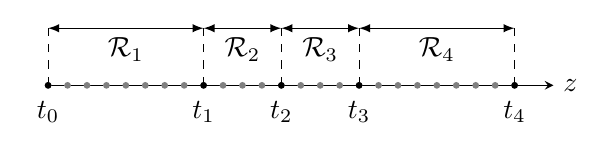
\begin{tikzpicture}
	\begin{axis}[width=8cm,height=4cm,xmin=0,xmax=6.5,xlabel=$z$,axis x line=middle,axis y line=none,xtick={0,2,3,4,6},xticklabels={$t_0$,$t_1$,$t_2$,$t_3$,$t_4$},xtick style={draw=none},every axis x label/.style={at=(current axis.right of origin),anchor=west},domain=0:6]
		\addplot[mark=*,mark size=1pt,only marks,color=gray] {0};
		\addplot[mark=*,mark size=1pt,only marks,color=black] coordinates{(0,0) (2,0) (3,0) (4,0) (6,0)};
		\draw[color=black,dashed] (0,0) -- (0,0.6);
		\draw[color=black,dashed] (2,0) -- (2,0.6);
		\draw[color=black,dashed] (3,0) -- (3,0.6);
		\draw[color=black,dashed] (4,0) -- (4,0.6);
		\draw[color=black,dashed] (6,0) -- (6,0.6);
		\draw[latex-latex] (0,0.6) -- (2,0.6) node[below,midway]{$\mathcal{R}_1$};
		\draw[latex-latex] (2,0.6) -- (3,0.6) node[below,midway]{$\mathcal{R}_2$};
		\draw[latex-latex] (3,0.6) -- (4,0.6) node[below,midway]{$\mathcal{R}_3$};
		\draw[latex-latex] (4,0.6) -- (6,0.6) node[below,midway]{$\mathcal{R}_4$};
	\end{axis}
\end{tikzpicture}

			}
			\caption{The decision thresholds are selected from fine-grained discrete energy levels instead of continuous space, and each decision region consists of at least one neighbor energy bins.}
			\label{fi:discrete_outputs}
		\end{figure}
		As shown in Fig. \ref{fi:discrete_outputs}, by introducing the extra analog-to-digital conversion step, we can group adjacent high-resolution energy bins for backscatter decision regions.
		Thus, problem \eqref{op:decision_threshold} is recast as
		\begin{maxi!}
			{\scriptstyle{\boldsymbol{t} \in \mathcal{T}^{L+1}}}{I_{\mathrm{B}}(x_{\mathcal{K}};\hat{x}_{\mathcal{K}})}{\label{op:decision_threshold_discrete}}{\label{ob:decision_threshold_discrete}}
			\addConstraint{\eqref{co:sequential_threshold},}
		\end{maxi!}
		which can be solved by existing rate-optimal sequential quantizer designs for \gls{dmc}.
		To obtain global optimal solution, \cite{He2021} started from the quadrangle inequality and proposed a \gls{dp} method accelerated by the \gls{smawk} algorithm with computational complexity $\mathcal{O}\bigl(L^2(\mathrm{card}(\mathcal{T})-L)\bigr)$, while \cite{Nguyen2020a} started from the optimality condition for three neighbor thresholds and presented a traverse-then-bisect algorithm with complexity $\mathcal{O}\bigl(\mathrm{card}(\mathcal{T})L\log(\mathrm{card}(\mathcal{T})L)\bigr)$.
		In Section \ref{se:simulation_results}, both schemes will be compared with the \gls{ml} thresholding \cite{Qian2019}
		\begin{equation}
			t_{l}^{\text{\gls{ml}}} = N \frac{\sigma_{l-1}^2 \sigma_{l}^2}{\sigma_{l-1}^2 - \sigma_{l}^2} \log \frac{\sigma_{l-1}^2}{\sigma_{l}^2}, \quad l \in \mathcal{L} \setminus \{L\},
			\label{eq:detection_threshold_ml}
		\end{equation}
		which is generally suboptimal for problem \eqref{op:decision_threshold} except when all nodes are with equiprobable inputs.
	\end{subsection}
\end{section}

\begin{section}{Simulation Results}
	In this section, we provide numerical results to evaluate the proposed input distribution, active beamforming, and backscatter decision design for the RIScatter system in Fig. \ref{fi:riscatter_network}.
	We assume the AP-user distance is \qty{10}{\meter} and at least one RIScatter nodes are randomly dropped in a disk centered at the user with radius \qty{2}{\meter}.
	% The \gls{ap} is with an average power budget $P=\qty{36}{\dBm}$, the nodes employs $M$-\gls{qam} with amplitude scattering ratio $\alpha=0.5$, the user is with average noise power $\sigma_v^2=\qty{-40}{\dBm}$, and the symbol period ratio is $N=20$.
	The \gls{ap} is with an average transmit power budget $P=\qty{36}{\dBm}$, all nodes employs $M$-\gls{qam} with amplitude scattering ratio $\alpha=0.5$, and the user is with average noise power $\sigma_v^2=\qty{-40}{\dBm}$.
	% Q=4 and symbol period ratio is $N=20$.
	For all channels involved, we consider a distance-dependent path loss model
	\begin{equation}
		L(d) = L_0 \biggl(\frac{d_0}{d}\biggr)^\gamma,
	\end{equation}
	together with a Rician fading model
	\begin{equation}
		\boldsymbol{H} = \sqrt{\frac{\kappa}{1+\kappa}} \bar{\boldsymbol{H}} + \sqrt{\frac{1}{1+\kappa}} \tilde{\boldsymbol{H}},
	\end{equation}
	where $d$ is the transmission distance, $L_0=-\qty{30}{\dB}$ is the reference path loss at distance $d_0=\qty{1}{\meter}$, $\kappa$ is the Rician $K$-factor, $\bar{\boldsymbol{H}}$ is the deterministic line-of-sight component with entries of unit magnitude, and $\tilde{\boldsymbol{H}}$ is the Rayleigh fading component with entries in standard \gls{iid} \gls{cscg} distribution.
	We choose $\gamma_{\mathrm{D}}=2.6$, $\gamma_{\mathrm{F}}=2.4$, $\gamma_{\mathrm{B}}=2$, and $\kappa_{\mathrm{D}}=\kappa_{\mathrm{F}}=\kappa_{\mathrm{B}}=5$ for direct, forward and backward links.
	The finite threshold domain $\mathcal{T}$ is obtained by $b$-bit uniform discretization over the critical interval defined by the confidence bounds of edge hypotheses (i.e., lower bound of $\mathcal{H}_1$ and upper bound of $\mathcal{H}_L$) with confidence level $1-\varepsilon$, where $b=9$ and $\varepsilon=\num{1e-3}$.
	% The achievable primary-(sum-)backscatter rate point is defined as $(I_{\mathrm{P}}(s;y),)$
	All average achievable rate points/regions are evaluated over \num{1000} realizations, and the parameters remain fixed unless otherwise specified.

	\begin{subsection}{Evaluation of Proposed Algorithms}
		\begin{subsubsection}{Initialization}
			To characterize the achievable rate region, we progressively obtain all boundary points by successively increasing the primary priority $\rho$ and solving problem \eqref{op:weighted_sum_rate}.
			At $\rho=0$ where backscatter performance is absolutely prioritized, we initialize Algorithm \ref{al:input_distribution} and \ref{al:active_beamforming} by uniform input distribution and \gls{mrt} towards sum cascaded channel $\sum_{k} \boldsymbol{h}_{\mathrm{C},k}^H$, respectively.
			At the following points, both algorithms are initialized by the final solutions at the previous point.
		\end{subsubsection}

		\begin{subsubsection}{Convergence}
			\begin{figure}[!t]
				\centering
				\resizebox{0.75\columnwidth}{!}{
					% This file was created by matlab2tikz.
%
%The latest updates can be retrieved from
%  http://www.mathworks.com/matlabcentral/fileexchange/22022-matlab2tikz-matlab2tikz
%where you can also make suggestions and rate matlab2tikz.
%
\definecolor{mycolor1}{rgb}{0.00000,0.44706,0.74118}%
\definecolor{mycolor2}{rgb}{0.85098,0.32549,0.09804}%
\definecolor{mycolor3}{rgb}{0.92941,0.69412,0.12549}%
%
\begin{tikzpicture}

\begin{axis}[%
width=4.053in,
height=0.919in,
at={(0.68in,2.887in)},
scale only axis,
xmin=0,
xmax=120,
ymin=0.113244880454575,
ymax=0.116102304831398,
axis background/.style={fill=white},
xmajorgrids,
ymajorgrids,
legend style={at={(0.97,0.03)}, anchor=south east, legend cell align=left, align=left, draw=white!15!black},
title style={font=\Large},
label style={font=\Large},
ticklabel style={font=\large},
legend style={font=\large},
yticklabel=\pgfkeys{/pgf/number format/.cd,fixed,precision=3}\pgfmathprintnumber{\tick}
]
\addplot [color=mycolor1, line width=2.0pt, mark=o, mark options={solid, mycolor1}]
  table[row sep=crcr]{%
0	0.113244880454575\\
10	0.114358992707155\\
20	0.114956255981364\\
30	0.115310191711237\\
40	0.115536251457935\\
50	0.11568965371294\\
60	0.115799285291346\\
70	0.115881218617581\\
80	0.115944814587431\\
90	0.115995739004593\\
100	0.116037546854275\\
110	0.116072549598378\\
120	0.116102304831398\\
};
\addlegendentry{KKT}

\end{axis}

\begin{axis}[%
width=4.053in,
height=0.919in,
at={(0.68in,1.67in)},
scale only axis,
xmin=0,
xmax=14,
ymin=0.116354276985174,
ymax=0.157617738080098,
ylabel style={font=\color{white!15!black}},
ylabel={Weighed Sum-Rate},
axis background/.style={fill=white},
xmajorgrids,
ymajorgrids,
legend style={at={(0.97,0.03)}, anchor=south east, legend cell align=left, align=left, draw=white!15!black},
title style={font=\Large},
label style={font=\Large},
ticklabel style={font=\large},
legend style={font=\large},
yticklabel=\pgfkeys{/pgf/number format/.cd,fixed,precision=3}\pgfmathprintnumber{\tick}
]
\addplot [color=mycolor2, dashed, line width=2.0pt, mark=+, mark options={solid, mycolor2}]
  table[row sep=crcr]{%
0	0.116354276985174\\
1	0.134986216301261\\
2	0.137045463164113\\
3	0.14221149883543\\
4	0.143513293823474\\
5	0.148182976472748\\
6	0.148354041018766\\
7	0.150388146565952\\
8	0.151376635136393\\
9	0.15160915733737\\
10	0.15291935995385\\
11	0.156743857286177\\
12	0.157617738080098\\
13	0.157617738080098\\
};
\addlegendentry{PGD}

\end{axis}

\begin{axis}[%
width=4.053in,
height=0.919in,
at={(0.68in,0.453in)},
scale only axis,
xmin=0,
xmax=8,
xlabel style={font=\color{white!15!black}},
xlabel={Number of Iterations},
ymin=0,
ymax=0.765555326497281,
axis background/.style={fill=white},
xmajorgrids,
ymajorgrids,
legend style={at={(0.97,0.03)}, anchor=south east, legend cell align=left, align=left, draw=white!15!black},
title style={font=\Large},
label style={font=\Large},
ticklabel style={font=\large},
legend style={font=\large},
yticklabel=\pgfkeys{/pgf/number format/.cd,fixed,precision=3}\pgfmathprintnumber{\tick}
]
\addplot [color=mycolor3, dotted, line width=2.0pt, mark=square, mark options={solid, mycolor3}]
  table[row sep=crcr]{%
0	0.113244880454575\\
1	0.159820508450486\\
2	0.271161604498627\\
3	0.403558255259651\\
4	0.594995557319089\\
5	0.748644776092643\\
6	0.764477923292286\\
7	0.765555325740019\\
8	0.765555326497281\\
};
\addlegendentry{BCD}

\end{axis}
\end{tikzpicture}%
				}
				\caption{Convergence behavior of the proposed algorithms for $\rho=0$.}
				\label{fi:wsr_convergence}
			\end{figure}

			In Fig. \ref{fi:wsr_convergence}, we plot the weighted sum of primary and total backscatter rates at $\rho=0$ for \gls{kkt}, \gls{pgd} (on the first call within \gls{bcd}) and \gls{bcd} algorithms in each iteration.
			For $K=8$ and $M=2$, Algorithm \ref{al:input_distribution} typically takes around \num{100} fast iterations over closed-form expression \eqref{eq:input_kkt_solution} to converge to the \gls{kkt} input distribution.
			For $Q=4$, around \num{10} iterations are required for Algorithm \ref{al:active_beamforming} to converge, where the gradient needs to be computed by \eqref{eq:weighted_sum_mutual_information_gradient} and the step size needs to be refined by \gls{bls}.
			In comparison, the \gls{bcd} algorithm typically requires at most \num{5} iterations to converge.
			At the following rate points (not presented), the convergence of all three algorithms become much faster thanks to the progressive initialization.
			Overall, we conclude the proposed algorithms are able to converge within moderate iterations and provide significant rate benefits for the RIScatter system.
		\end{subsubsection}
	\end{subsection}

	\begin{subsection}{Comparison of Scattering Applications}
		% TODO SR analysis can achieve large rate at the cost of large N; RIScatter can achieve slightly lower rate at the same N, but also preserves primary performance for smaller N
		% TODO tradeoff between primary (RIScatter, no SIC) and backscatter (SR, SIC)
		% ! SR assume very large N for primary rate analysis. However, in such cases SIC is questionable as energy detection over received signal as BBC is already good enough and non-coherent detection can also achieve reasonable performance?
		% TODO when primary symbols are determined, optimal input distribution at high backscatter SNR is equiprobable for any detection (signal/energy)
		% TODO (I(X_1;Y_1),I(X_2;Y_2))
		% For a fair comparison, we consider the setup in Fig. \ref{fi:riscatter_network} and employ \gls{ml} backscatter energy detection for these scattering applications:
		% For a fair comparison, we consider the setup in Fig. \ref{fi:riscatter_network} with \gls{ml} backscatter energy detection for these scattering applications (except \gls{sr}):
		% For a fair comparison with RIScatter, we consider the setup in Fig. \ref{fi:riscatter_network} and evaluate the achievable rate pairs for these scattering applications:
		% We consider the setup in Fig. \ref{fi:riscatter_network} and compare the achievable rate pairs of RIScatter and these scattering applications:
		On top of the setup in Fig. \ref{fi:riscatter_network}, we compare the achievable rate pairs of RIScatter and these scattering applications:
		\begin{itemize}
			\item \emph{\gls{bbc}:}
			The primary symbol becomes deterministic $s[n]=1$ and the receive signal at each primary block is
			\begin{equation}
				% y^{\text{\gls{bbc}}}[n] = \boldsymbol{h}_{\mathrm{E}}^H(x_{\mathcal{K}}) \boldsymbol{w} + v[n],
				y^{\text{\gls{bbc}}}[n] = \Bigl(\boldsymbol{h}_{\mathrm{D}}^H + \sum_{k} \alpha_k \boldsymbol{h}_{\mathrm{C},k}^H x_k\Bigr) \boldsymbol{w} + v[n],
			\end{equation}
			% which follows non-zero mean complex Gaussian distribution $\mathcal{CN}\bigl(\boldsymbol{h}_{\mathrm{E}}^H(x_{m_{\mathcal{K}}}) \boldsymbol{w},\sigma_v^2\bigr)$ under hypothesis $\mathcal{H}_{m_{\mathcal{K}}}$.
			which follows non-zero mean complex Gaussian distribution $\mathcal{CN}\bigl((\boldsymbol{h}_{\mathrm{D}}^H + \sum_{k} \alpha_k \boldsymbol{h}_{\mathrm{C},k}^H x_{m_k}) \boldsymbol{w},\sigma_v^2\bigr)$ under hypothesis $\mathcal{H}_{m_{\mathcal{K}}}$.
			% \sum_{k} \alpha_k \boldsymbol{h}_{\mathrm{C},k}^H x_k
			The corresponding \gls{pdf} of accumulated receive energy over $N$ primary blocks is
			\begin{equation}
				f^{\text{\gls{bbc}}}(z|\mathcal{H}_{m_{\mathcal{K}}}) = \frac{(z-\mu_{m_{\mathcal{K}}}^{\text{\gls{bbc}}})^{N-1} \exp \bigl(-(z-\mu_{m_{\mathcal{K}}}^{\text{\gls{bbc}}})/\sigma_v^2 \bigr)}{\sigma_v^{2N} (N-1)!},
				\label{eq:energy_distribution_bbc}
			\end{equation}
			% where $\mu_{m_{\mathcal{K}}}^{\text{\gls{bbc}}} \triangleq N \lvert \boldsymbol{h}_{\mathrm{E}}^H(x_{m_{\mathcal{K}}}) \boldsymbol{w} \rvert^2$.
			where $\mu_{m_{\mathcal{K}}}^{\text{\gls{bbc}}} \triangleq N \bigl\lvert \bigl(\boldsymbol{h}_{\mathrm{D}}^H + \sum_{k} \alpha_k \boldsymbol{h}_{\mathrm{C},k}^H x_{m_k}\bigr) \boldsymbol{w} \bigr\rvert^2$.
			The \gls{ml} decision threshold is derived as, $\forall l \in \mathcal{L} \setminus \{L\}$,
			\begin{equation}
				t_l^{\text{\gls{bbc}}} = \frac{\mu_{l-1}^{\text{\gls{bbc}}} \exp \bigl((\mu_{l-1}^{\text{\gls{bbc}}}-\mu_{l}^{\text{\gls{bbc}}})/\sigma_v^2 (N-1)\bigr) - \mu_{l}^{\text{\gls{bbc}}}}{\exp \bigl((\mu_{l-1}^{\text{\gls{bbc}}}-\mu_{l}^{\text{\gls{bbc}}})/\sigma_v^2 (N-1)\bigr) - 1}.
				\label{eq:detection_threshold_ml_bbc}
			\end{equation}
			\item \emph{\gls{ambc}:} The user decodes both links independently and semi-coherently by treating the other as interference or uncertainty.
			Hence, the primary achievable rate can be approximated by\footnote{To provide a preliminary benchmark, we approximate the unknown signal components from finite-input backscatter sources by independent interference from Gaussian sources.}
			\begin{equation}
				I_{\mathrm{P}}^{\text{\gls{ambc}}}(s;y) \approx \log \Bigl(1 + \frac{\lvert\boldsymbol{h}_{\mathrm{D}}^H\boldsymbol{w}\rvert^2}{\sum_{k}\lvert \alpha_k \boldsymbol{h}_{\mathrm{C},k}^H \boldsymbol{w}\rvert^2+\sigma_v^2}\Bigr),
			\end{equation}
			while the total backscatter rate follows \eqref{eq:backscatter_mutual_information} with uniform input distribution.
			\item \emph{\gls{sr}:} For a sufficiently large $N$, the primary ergodic rate under semi-coherent detection asymptotically approaches \eqref{eq:primary_mutual_information} with uniform input distribution \cite{Long2020a}.
			When $s[n]$ is successfully decoded and the direct interference $\boldsymbol{h}_{\mathrm{D}}^H \boldsymbol{w} s[n]$ is perfectly cancelled, the intermediate signal for backscatter detection is
			\begin{equation}
				\hat{y}^{\text{\gls{sr}}}[n] = \sum_{k} \alpha_k \boldsymbol{h}_{\mathrm{C},k}^H x_k \boldsymbol{w} s[n] + v[n],
			\end{equation}
			which only involves noise uncertainty under hypothesis $\mathcal{H}_{m_{\mathcal{K}}}$.
			% and follows non-zero mean complex Gaussian distribution $\mathcal{CN}\bigl(\sum_{k} \alpha_k \boldsymbol{h}_{\mathrm{C},k}^H x_k \boldsymbol{w} s[n],\sigma_v^2\bigr)$.
			By \gls{mrc} over $N$ primary blocks, the total achievable for nodes with equiprobable inputs is \cite{Wang2014a}
			\begin{equation}
				I_{\mathrm{B}}(x_{\mathcal{K}};\hat{y}_{\text{\gls{sr}}}) = K \log M - \frac{\epsilon}{M^K},
			\end{equation}
			where $\epsilon \triangleq \sum_{m_{\mathcal{K}}} \mathbb{E}_{\hat{v}} \log \sum_{m_{\mathcal{K}}'} \exp ( - {\lvert x_{m_{\mathcal{K}}} - x_{m_{\mathcal{K}}'} + \hat{v} \rvert^2}/{2 \sigma^2} )$ and $\hat{v} \sim \mathcal{CN}(0,\sigma_v^2/N)$.
			For a sufficiently large $N$, $\epsilon$ is negligible and the total backscatter rate approaches $K \log M$.
			\item \emph{\gls{ris}:} Since the backscatter symbol tuple $x_{\mathcal{K}}$ becomes deterministic, the total backscatter rate is zero and the primary achievable rate boils down to a special case of \eqref{eq:primary_mutual_information}
			\begin{equation}
				I_{\mathrm{P}}^{\text{\gls{ris}}}(s;y|x_{\mathcal{K}}) = I_{\mathrm{P}}(s;y|x_{m_{\mathcal{K}}^{\star}}) = \log \Bigl(1 + \frac{\lvert \boldsymbol{h}_{\mathrm{E}}^H(x_{m_{\mathcal{K}}^{\star}}) \boldsymbol{w} \rvert^2}{\sigma_v^2}\Bigr),
			\end{equation}
			where $m_{\mathcal{K}}^{\star} = \arg \max_{m_{\mathcal{K}}} I_{\mathrm{P}}(s;y|x_{m_{\mathcal{K}}})$.
		\end{itemize}
		\begin{figure}[!t]
			\centering
			\resizebox{0.65\columnwidth}{!}{
				% This file was created by matlab2tikz.
%
%The latest updates can be retrieved from
%  http://www.mathworks.com/matlabcentral/fileexchange/22022-matlab2tikz-matlab2tikz
%where you can also make suggestions and rate matlab2tikz.
%
\definecolor{mycolor1}{rgb}{0.30100,0.74500,0.93300}%
\definecolor{mycolor2}{rgb}{0.46600,0.67400,0.18800}%
\definecolor{mycolor3}{rgb}{0.49400,0.18400,0.55600}%
\definecolor{mycolor4}{rgb}{0.92900,0.69400,0.12500}%
\definecolor{mycolor5}{rgb}{0.85000,0.32500,0.09800}%
\definecolor{mycolor6}{rgb}{0.00000,0.44700,0.74100}%
%
\begin{tikzpicture}

\begin{axis}[%
width=4.079in,
height=1.587in,
at={(0.684in,0.361in)},
scale only axis,
xmin=0,
xmax=6.5227548374066,
xlabel style={font=\color{white!15!black}},
xlabel={Primary Rate [bits/s/Hz]},
ymin=0,
ymax=2,
ylabel style={font=\color{white!15!black}},
ylabel={Backscatter\\Rate [bits/BB]},
axis background/.style={fill=white},
xmajorgrids,
ymajorgrids,
legend style={at={(0.03,0.03)}, anchor=south west, legend cell align=left, align=left, draw=white!15!black},
align=center,
title style={font=\LARGE},
label style={font=\LARGE},
ticklabel style={font=\Large},
legend style={font=\Large},
reverse legend,
every axis plot/.append style={line width=2pt}
]
\addplot [color=mycolor1, line width=2.0pt, mark=triangle, mark options={solid, rotate=180, mycolor1}]
  table[row sep=crcr]{%
6.33724402501803	1.39764296268229\\
0	1.39764296268229\\
0	0\\
6.52275483678685	0\\
6.52275483678685	2.37312052924553e-08\\
6.38739454470992	1.3235811846854\\
6.35422040211439	1.38916612409166\\
6.34857862205488	1.39386686170527\\
6.3445353675389	1.39608085009443\\
6.34291602910554	1.3966977322109\\
6.34149846039129	1.39711118534274\\
6.34024731759122	1.39737797077851\\
6.3391350240222	1.3975379071887\\
6.33862394227692	1.39758701988787\\
6.33813974610465	1.39761939115801\\
6.33795313341839	1.39762818964178\\
6.33777036860279	1.39763482338317\\
6.3375913342378	1.3976394187338\\
6.33741590881855	1.39764209463684\\
6.33724402501803	1.39764296268229\\
};
\addlegendentry{RIScatter}

\addplot[only marks, mark=triangle, mark options={}, mark size=2.3570pt, draw=mycolor2] table[row sep=crcr]{%
x	y\\
6.5227548374066	0\\
};
\addlegendentry{RIS}

\addplot[only marks, mark=+, mark options={}, mark size=3.5355pt, draw=mycolor3] table[row sep=crcr]{%
x	y\\
6.34321982467796	2\\
};
\addlegendentry{SR}

\addplot[only marks, mark=x, mark options={}, mark size=3.5355pt, draw=mycolor4] table[row sep=crcr]{%
x	y\\
5.90778796357092	1.34857377961699\\
};
\addlegendentry{AmBC}

\addplot[only marks, mark=square, mark options={}, mark size=2.5000pt, draw=mycolor5] table[row sep=crcr]{%
x	y\\
0	1.99999999999997\\
};
\addlegendentry{BBC}

\addplot[only marks, mark=o, mark options={}, mark size=2.7386pt, draw=mycolor6] table[row sep=crcr]{%
x	y\\
6.34314881160129	0\\
};
\addlegendentry{Legacy}

\end{axis}
\end{tikzpicture}%
			}
			\caption{Typical achievable rate points of scattering applications for $Q=1$, $K=1$, $M=4$ and $N=1000$.}
			\label{fi:region_comparison}
		\end{figure}

		Fig. \ref{fi:region_comparison} presents the typical achieve rate points of different scattering applications for $Q=1$, $K=1$, $M=4$ and $N=1000$.
		First, we observe both \gls{bbc} and \gls{sr} can achieve the highest backscatter rate with coherent detection over the receive energy and intermediate signal, respectively.
		This is because repetition coding with \gls{mrc} over $N$ primary blocks effectively increases the backscatter \gls{snr} by $N$ times, and the information loss due to the signal-to-energy conversion on top may be insignificant.
		However, the asymptotic primary and backscatter rate analysis only provides upper bounds for \gls{sr}.
		Using a very large $N$ not only reduces the system throughput\footnote{For example, Wi-Fi sampling rate is \qty{20}{\MHz} while \gls{rfid} load switching speed varies between \num{100}s of \unit{\kHz} to \num{10}s of \unit{\MHz} \cite{Torres2021}, corresponding to a typical symbol period ratio $N$ between \num{1} and \num{100}.} but also requires the operation-intensive \gls{sic} over each primary block.
		When the duration of primary and backscatter symbol are comparable, the randomly scattered signals should be modelled as interference to primary link rather than quasi-static multipath components, and the achievable rate point of \gls{sr} will move towards the origin.
		On the other hand, RIScatter provides a lower backscatter rate than \gls{bbc} and \gls{sr} due to semi-coherent detection, but preserves the primary rate benefit for arbitrary $N$.



		% TODO SR analysis can achieve large rate at the cost of large N; RIScatter can achieve slightly lower rate at the same N, but also preserves primary performance for smaller N
		% TODO tradeoff between primary (RIScatter, no SIC) and backscatter (SR, SIC)
		% ! SR assume very large N for primary rate analysis. However, in such cases SIC is questionable as energy detection over received signal as BBC is already good enough and non-coherent detection can also achieve reasonable performance?
		% TODO when primary symbols are determined, optimal input distribution at high backscatter SNR is equiprobable for any detection (signal/energy)
		% TODO Wi-Fi sampling rate 20 MHz (symbol period 50 nS), RFID symbol rate/load switching speed 100s KHz to 10s MHz [Backscatter Communications], fast load switching speed is key for high data rate - symbol ratio is not very large

		Backscatter advantage of SR using SIC is prominent for a smaller N
		% correlation by double modulation improves the detection performance
		% when $N$ is sufficiently large.
	\end{subsection}

	\begin{subsection}{Input Distribution under Different Weights}
		\begin{figure}[!t]
			\centering
			\resizebox{0.65\columnwidth}{!}{
				% This file was created by matlab2tikz.
%
%The latest updates can be retrieved from
%  http://www.mathworks.com/matlabcentral/fileexchange/22022-matlab2tikz-matlab2tikz
%where you can also make suggestions and rate matlab2tikz.
%
\definecolor{mycolor1}{rgb}{0.00000,0.44706,0.74118}%
\definecolor{mycolor2}{rgb}{0.85098,0.32549,0.09804}%
\definecolor{mycolor3}{rgb}{0.92941,0.69412,0.12549}%
\definecolor{mycolor4}{rgb}{0.49412,0.18431,0.55686}%
%
\begin{tikzpicture}

\begin{axis}[%
width=4.079in,
height=3.432in,
at={(0.684in,0.463in)},
scale only axis,
xmin=1,
xmax=4,
xtick={1, 2, 3, 4},
xlabel style={font=\color{white!15!black}},
xlabel={Reflection State},
ymin=0,
ymax=1,
ytick={  0, 0.2, 0.4, 0.6, 0.8,   1},
ylabel style={font=\color{white!15!black}},
ylabel={Probability Distribution},
axis background/.style={fill=white},
xmajorgrids,
ymajorgrids,
legend style={legend cell align=left, align=left, draw=white!15!black},
title style={font=\LARGE},
label style={font=\LARGE},
ticklabel style={font=\Large},
legend style={font=\Large}
]
\addplot [color=mycolor1, line width=2.0pt, mark=o, mark options={solid, mycolor1}]
  table[row sep=crcr]{%
1	5.58936301883394e-08\\
2	0.494967846198009\\
3	0.505032051077508\\
4	4.68308531955441e-08\\
};
\addlegendentry{$\rho =0$}

\addplot [color=mycolor2, dashed, line width=2.0pt, mark=+, mark options={solid, mycolor2}]
  table[row sep=crcr]{%
1	3.50493170830856e-09\\
2	0.586489834632108\\
3	0.413510159250847\\
4	2.6121135277758e-09\\
};
\addlegendentry{$\rho =0.1$}

\addplot [color=mycolor3, dotted, line width=2.0pt, mark=square, mark options={solid, mycolor3}]
  table[row sep=crcr]{%
1	1.54239700394178e-10\\
2	0.770075793479604\\
3	0.229924206275344\\
4	9.08124388871134e-11\\
};
\addlegendentry{$\rho =0.25$}

\addplot [color=mycolor4, dashdotted, line width=2.0pt, mark=x, mark options={solid, mycolor4}]
  table[row sep=crcr]{%
1	1.62167297049731e-12\\
2	0.999999185020827\\
3	8.14977502370884e-07\\
4	4.9209962545264e-14\\
};
\addlegendentry{$\rho =1$}

\end{axis}
\end{tikzpicture}%
			}
			\caption{Typical reflection state distribution under different weights for $Q=1$, $K=1$, $M=4$ and $N=20$.}
			\label{fi:distribution_weights}
		\end{figure}
		The objective of this study is to demonstrate each RIScatter node can adjust its input distribution based on \gls{csi} and link priority to balance backscatter modulation and passive beamforming.
		For this aim, we evaluate the \gls{kkt} input distribution by Algorithm \ref{al:input_distribution} for a single node under different weights in Fig. \ref{fi:distribution_weights}.
		We observe that as $\rho$ increases from \num{0} to \num{1}, the \gls{kkt} input distribution
		gradually progresses from slightly skewed to completely biased.
		For $\rho=0$ where backscatter performance is absolutely prioritized, the \gls{csi}-adaptive channel coding at the RIScatter node provides higher backscatter rate than conventional \gls{bc} and \gls{sr} nodes with equiprobable inputs, and some states may end up unused since they cannot produce enough energy difference over the existing alphabet.
		On the other hand, for $\rho=1$ where primary performance is absolutely prioritized, the input probability is \num{1} at the state that maximizes the primary equivalent channel strength, and \num{0} at the others.
		In this case, the reflection pattern over time is fully deterministic, and the RIScatter node indeed boils down to a \gls{ris} element with discrete phase shifts.
		Those observations meet our s that RIScatter nodes include scattering sources of \gls{bc}/\gls{sr} and reflecting elements of \gls{ris} as special cases, and generalize backscatter modulation and passive beamforming from the perspective of input distribution design.
		For the \gls{bcd} algorithm, we choose the \gls{kkt} input distribution by Algorithm \ref{al:input_distribution}, the \gls{pgd} active beamforming by Algorithm \ref{al:active_beamforming}, and the \gls{smawk} decision threshold by \cite{He2021} as reference.
	\end{subsection}

	% \begin{subsection}{Achievable Rates versus Energy Discretization Bits}
	% 	\begin{figure}[!t]
	% 		\subfloat[Primary Rate\label{fi:rate_bits_primary}]{
	% 			\resizebox{0.48\columnwidth}{!}{
	% 				% This file was created by matlab2tikz.
%
%The latest updates can be retrieved from
%  http://www.mathworks.com/matlabcentral/fileexchange/22022-matlab2tikz-matlab2tikz
%where you can also make suggestions and rate matlab2tikz.
%
\definecolor{mycolor1}{rgb}{0.00000,0.44706,0.74118}%
%
\begin{tikzpicture}

\begin{axis}[%
width=4.036in,
height=3.396in,
at={(0.677in,0.458in)},
scale only axis,
xmin=4,
xmax=7,
xtick={4, 5, 6, 7},
xlabel style={font=\color{white!15!black}},
xlabel={Energy Discretization Bits},
ymin=7.73539873944944,
ymax=9.73539873944944,
ylabel style={font=\color{white!15!black}},
ylabel={Primary Rate [bits/s/Hz]},
axis background/.style={fill=white},
xmajorgrids,
ymajorgrids,
legend style={at={(0.97,0.03)}, anchor=south east, legend cell align=left, align=left, draw=white!15!black},
title style={font=\huge},
label style={font=\huge},
ticklabel style={font=\LARGE},
legend style={font=\LARGE},
scaled y ticks=false,
y tick label style={/pgf/number format/.cd, fixed, precision=2}
]
\addplot [color=mycolor1, line width=2.0pt, mark=o, mark options={solid, mycolor1}]
  table[row sep=crcr]{%
4	8.73539873944944\\
5	8.73539873944944\\
6	8.73539873944944\\
7	8.73539873944944\\
};
\addlegendentry{Primary rate}

\end{axis}
\end{tikzpicture}%
	% 			}
	% 		}
	% 		\subfloat[Total Backscatter Rate\label{fi:rate_bits_backscatter}]{
	% 			\resizebox{0.48\columnwidth}{!}{
	% 				% This file was created by matlab2tikz.
%
%The latest updates can be retrieved from
%  http://www.mathworks.com/matlabcentral/fileexchange/22022-matlab2tikz-matlab2tikz
%where you can also make suggestions and rate matlab2tikz.
%
\definecolor{mycolor1}{rgb}{0.85098,0.32549,0.09804}%
%
\begin{tikzpicture}

\begin{axis}[%
width=3.972in,
height=3.353in,
at={(0.666in,0.453in)},
scale only axis,
xmin=4,
xmax=7,
xtick={4, 5, 6, 7},
xlabel style={font=\color{white!15!black}},
xlabel={Energy Discretization Bits},
ymin=0,
ymax=1,
ylabel style={font=\color{white!15!black}},
ylabel={Total Backscatte Rate [bits/BSP]},
axis background/.style={fill=white},
xmajorgrids,
ymajorgrids,
legend style={at={(0.97,0.03)}, anchor=south east, legend cell align=left, align=left, draw=white!15!black},
title style={font=\huge},
label style={font=\huge},
ticklabel style={font=\LARGE},
legend style={font=\LARGE},
scaled y ticks=false,
y tick label style={/pgf/number format/.cd, fixed, precision=2}
]
\addplot [color=mycolor1, dashed, line width=2.0pt, mark=+, mark options={solid, mycolor1}]
  table[row sep=crcr]{%
4	0.0398393854476695\\
5	0.655086014342697\\
6	0.655095223157023\\
7	0.647363955350682\\
};
\addlegendentry{Total backscatter rate}

\end{axis}
\end{tikzpicture}%
	% 			}
	% 		}
	% 		\caption{Average achievable primary and total backscatter rates for different energy discretization bits for $\rho=0$.}
	% 		\label{fi:rate_bits}
	% 	\end{figure}
	% 	We now reveal how the analog-to-digital conversion of feasible threshold domain from $\mathbb{R}_+^{L+1}$ to $\mathcal{T}^{L+1}$ affects the average RIScatter performance.
	% 	For a fixed input distribution and active beamforming, Fig. \ref{fi:rate_bits} shows the impact of energy discretization bits $b$ on the average achievable rates when $\rho=0$.
	% 	We observe the primary rate is a constant for different $b$ as expected from Remark \ref{re:backscatter_decision}.
	% 	This conclusion holds for arbitrary $\rho$ because the randomness of reflection patterns over time can always be eliminated upon successful backscatter decoding.
	% 	When the nodes transmit at non-zero total rate, the user can re-encode backscatter messages to recover their reflection patterns at each primary block.
	% 	Otherwise, the reflection patterns of all nodes are fully deterministic, and the state index tuple can be fed back to the user together with \gls{csi}.
	% 	We also notice increasing $b$ boosts the total backscatter rate and the benefit becomes marginal when $b$ is sufficiently large ($2^b \gg \mathrm{card}(\mathcal{L})$).
	% 	This is because a larger $b$ allows the decision regions to be constructed from narrower energy bins, which mitigates the transformation loss from problem \eqref{op:decision_threshold} to \eqref{op:decision_threshold_discrete}.
	% 	Therefore, we conclude a proper selection of $b$ is the key to balance backscatter performance and computational complexity.
	% \end{subsection}

	\begin{subsection}{Rate Region by Different Schemes}
		% \begin{figure}[!t]
		% 	\centering
		% 	\subfloat[Input Distribution\label{fi:region_distribution}]{
		% 		\resizebox{0.65\columnwidth}{!}{
		% 			% This file was created by matlab2tikz.
%
%The latest updates can be retrieved from
%  http://www.mathworks.com/matlabcentral/fileexchange/22022-matlab2tikz-matlab2tikz
%where you can also make suggestions and rate matlab2tikz.
%
\definecolor{mycolor1}{rgb}{0.00000,0.44706,0.74118}%
\definecolor{mycolor2}{rgb}{0.85098,0.32549,0.09804}%
\definecolor{mycolor3}{rgb}{0.92941,0.69412,0.12549}%
\definecolor{mycolor4}{rgb}{0.49412,0.18431,0.55686}%
\definecolor{mycolor5}{rgb}{0.46667,0.67451,0.18824}%
\definecolor{mycolor6}{rgb}{0.30196,0.74510,0.93333}%
\definecolor{mycolor7}{rgb}{0.63529,0.07843,0.18431}%
%
\begin{tikzpicture}

	\begin{axis}[%
			width=4.014in,
			height=3.389in,
			at={(0.673in,0.457in)},
			scale only axis,
			xmin=6,xmax=6.55,
			xtick={6,6.1,6.2,6.3,6.4,6.5},
			xlabel style={font=\color{white!15!black}},
			xlabel={Primary Rate [bits/s/Hz]},
			ymin=0,
			ymax=0.258249123037508,
			ylabel style={font=\color{white!15!black}},
			ylabel={Total Backscatter Rate [bits/BB]},
			axis background/.style={fill=white},
			xmajorgrids,
			ymajorgrids,
			legend style={at={(0.03,0.03)}, anchor=south west, legend cell align=left, align=left, draw=white!15!black},
			title style={font=\LARGE},
			label style={font=\LARGE},
			ticklabel style={font=\Large},
			legend style={font=\Large},
			scaled y ticks=false,
			y tick label style={/pgf/number format/.cd, fixed, precision=2}
		]
		\addplot [color=mycolor1, line width=2.0pt, mark=o, mark options={solid, mycolor1}]
		table[row sep=crcr]{%
				6.32146282014783	0.135298434401071\\
				0	0.135298434401071\\
				0	0\\
				6.54733712865232	0\\
				6.54517433822466	0.00774868535999835\\
				6.50756053444898	0.0675347647522537\\
				6.47890595069851	0.0908447067770361\\
				6.4405754582915	0.111410986078138\\
				6.41906097335963	0.119575938134352\\
				6.39711048749103	0.125961202920399\\
				6.375794485304	0.130496464040102\\
				6.35566511647813	0.13338720543392\\
				6.34622485273269	0.134291841616495\\
				6.33755099968818	0.134871348283307\\
				6.3341180598223	0.135032749667558\\
				6.33078786275436	0.135153660987559\\
				6.3275979313462	0.135235752926375\\
				6.32449832330173	0.135283108344685\\
				6.32146282014783	0.135298434401071\\
			};
		\addlegendentry{Exhaustion}

		\addplot [color=mycolor2, dashed, line width=2.0pt, mark=+, mark options={solid, mycolor2}]
		table[row sep=crcr]{%
				6.32141918409994	0.135302553290759\\
				0	0.135302553290759\\
				0	0\\
				6.54617494292906	0\\
				6.54617494292906	5.35569540967736e-08\\
				6.54395549026001	0.00794380155151132\\
				6.50571395400754	0.0685517046188535\\
				6.47725030932065	0.0915613607821624\\
				6.43904818034038	0.111868185202614\\
				6.41734122875771	0.119998466631658\\
				6.39569411793482	0.126224654256524\\
				6.37478946505091	0.130639435722587\\
				6.35513830914346	0.133439138952041\\
				6.34596989012747	0.134312547131226\\
				6.33728397409874	0.134887798900337\\
				6.33394436296369	0.135043581861458\\
				6.33067909442514	0.135160647084426\\
				6.32748262520049	0.135241405287329\\
				6.32435855863608	0.135287987095764\\
				6.32141918409994	0.135302553290759\\
			};
		\addlegendentry{KKT}

		\addplot [color=mycolor3, dotted, line width=2.0pt, mark=square, mark options={solid, mycolor3}]
		table[row sep=crcr]{%
				6.33038216910371	0.258249123037508\\
				0	0.258249123037508\\
				0	0\\
				6.54733712865225	0\\
				6.54733712865225	9.63577398919082e-15\\
				6.53818045939347	0.0325698770891707\\
				6.43706862579333	0.205987678214288\\
				6.40319420024859	0.234129375981137\\
				6.37756789518431	0.24814619770397\\
				6.36712369262437	0.252123967734036\\
				6.35793773244948	0.25480261208027\\
				6.3498258540104	0.256532319837123\\
				6.34261469311561	0.257569015164329\\
				6.33930342588844	0.257887218672394\\
				6.33616929824435	0.258096765396561\\
				6.33496269926005	0.258153654718521\\
				6.33378166469514	0.258196523198478\\
				6.33262379024928	0.258226244645555\\
				6.33149125428708	0.258243521141676\\
				6.33038216910371	0.258249123037508\\
			};
		\addlegendentry{Cooperation}

		\addplot [color=mycolor4, dashdotted, line width=2.0pt, mark=x, mark options={solid, mycolor4}]
		table[row sep=crcr]{%
				6.3353047399281	0.132538456219543\\
				0	0.132538456219543\\
				0	0\\
				6.54733712865224	0\\
				6.54733712865224	4.9616544470467e-15\\
				6.53883907987144	0.0173736087216158\\
				6.44100451648281	0.104073934077473\\
				6.40767165852713	0.118546491406672\\
				6.38231104047054	0.126127571777712\\
				6.37194304642766	0.128392528291276\\
				6.36281278709048	0.129987574291472\\
				6.35472791571861	0.131088141723972\\
				6.34753142631954	0.131822608691493\\
				6.34422575990388	0.13208245385162\\
				6.34109503581159	0.132282820185509\\
				6.33988891868859	0.132348288736295\\
				6.33870564827907	0.132406206639739\\
				6.33754869585191	0.132457094231239\\
				6.33641540465384	0.13250082882571\\
				6.3353047399281	0.132538456219543\\
			};
		\addlegendentry{Marginalization}

		\addplot [color=mycolor5, line width=2.0pt, mark=triangle, mark options={solid, mycolor5}]
		table[row sep=crcr]{%
				6.33515135931876	0.0104508384451561\\
				0	0.0104508384451561\\
				0	0\\
				6.54733712865225	0\\
				6.54733712865225	9.41351914512674e-17\\
				6.54566316113138	0.0018911689220282\\
				6.50449357170924	0.00614593506985847\\
				6.47104644280986	0.00857077717475668\\
				6.33515135931876	0.0104508384451561\\
			};
		\addlegendentry{Decomposition}

		\addplot [color=mycolor6, dashed, line width=2.0pt, mark=triangle, mark options={solid, rotate=180, mycolor6}]
		table[row sep=crcr]{%
				6.51905860474812	0.040829341410189\\
				0	0.040829341410189\\
				0	0\\
				6.5473371278862	0\\
				6.5473371278862	1.13550059120926e-09\\
				6.54539615692803	0.00510452797145521\\
				6.51905860474812	0.040829341410189\\
			};
		\addlegendentry{Randomization}

		\addplot [color=mycolor7, dotted, line width=2.0pt, mark=triangle, mark options={solid, rotate=270, mycolor7}]
		table[row sep=crcr]{%
				6.34050352716188	0.131452428942456\\
				6.34050352716188	0.131452428942456\\
				6.34050352716188	0.131452428942456\\
				6.34050352716188	0.131452428942456\\
				6.34050352716188	0.131452428942456\\
				0	0.131452428942456\\
				0	0\\
				6.34050352716188	0\\
				6.34050352716188	0.131452428942456\\
			};
		\addlegendentry{Equiprobable}

	\end{axis}

	\begin{axis}[%
			width=1.036in,
			height=1.039in,
			at={(1.543in,2.588in)},
			scale only axis,
			separate axis lines,
			every outer x axis line/.append style={black},
			every x tick label/.append style={font=\color{black}},
			every x tick/.append style={black},
			xmin=6.324,
			xmax=6.36,
			every outer y axis line/.append style={black},
			every y tick label/.append style={font=\color{black}},
			every y tick/.append style={black},
			ymin=0.129114533984272,
			ymax=0.137036286224687,
			axis background/.style={fill=white!90!black},
			xmajorgrids,
			ymajorgrids,
			title style={font=\LARGE},
			label style={font=\LARGE},
			ticklabel style={font=\Large},
			legend style={font=\Large},
			scaled y ticks=false,
			y tick label style={/pgf/number format/.cd, fixed, precision=3}
		]
		\addplot [color=mycolor1, line width=2.0pt, mark=o, mark options={solid, mycolor1}, forget plot]
		table[row sep=crcr]{%
				6.32146282014783	0.135298434401071\\
				0	0.135298434401071\\
				0	0\\
				6.54733712865232	0\\
				6.54517433822466	0.00774868535999835\\
				6.50756053444898	0.0675347647522537\\
				6.47890595069851	0.0908447067770361\\
				6.4405754582915	0.111410986078138\\
				6.41906097335963	0.119575938134352\\
				6.39711048749103	0.125961202920399\\
				6.375794485304	0.130496464040102\\
				6.35566511647813	0.13338720543392\\
				6.34622485273269	0.134291841616495\\
				6.33755099968818	0.134871348283307\\
				6.3341180598223	0.135032749667558\\
				6.33078786275436	0.135153660987559\\
				6.3275979313462	0.135235752926375\\
				6.32449832330173	0.135283108344685\\
				6.32146282014783	0.135298434401071\\
			};
		\addplot [color=mycolor2, dashed, line width=2.0pt, mark=+, mark options={solid, mycolor2}, forget plot]
		table[row sep=crcr]{%
				6.32141918409994	0.135302553290759\\
				0	0.135302553290759\\
				0	0\\
				6.54617494292906	0\\
				6.54617494292906	5.35569540967736e-08\\
				6.54395549026001	0.00794380155151132\\
				6.50571395400754	0.0685517046188535\\
				6.47725030932065	0.0915613607821624\\
				6.43904818034038	0.111868185202614\\
				6.41734122875771	0.119998466631658\\
				6.39569411793482	0.126224654256524\\
				6.37478946505091	0.130639435722587\\
				6.35513830914346	0.133439138952041\\
				6.34596989012747	0.134312547131226\\
				6.33728397409874	0.134887798900337\\
				6.33394436296369	0.135043581861458\\
				6.33067909442514	0.135160647084426\\
				6.32748262520049	0.135241405287329\\
				6.32435855863608	0.135287987095764\\
				6.32141918409994	0.135302553290759\\
			};
		\addplot [color=mycolor3, dotted, line width=2.0pt, mark=square, mark options={solid, mycolor3}, forget plot]
		table[row sep=crcr]{%
				6.33038216910371	0.258249123037508\\
				0	0.258249123037508\\
				0	0\\
				6.54733712865225	0\\
				6.54733712865225	9.63577398919082e-15\\
				6.53818045939347	0.0325698770891707\\
				6.43706862579333	0.205987678214288\\
				6.40319420024859	0.234129375981137\\
				6.37756789518431	0.24814619770397\\
				6.36712369262437	0.252123967734036\\
				6.35793773244948	0.25480261208027\\
				6.3498258540104	0.256532319837123\\
				6.34261469311561	0.257569015164329\\
				6.33930342588844	0.257887218672394\\
				6.33616929824435	0.258096765396561\\
				6.33496269926005	0.258153654718521\\
				6.33378166469514	0.258196523198478\\
				6.33262379024928	0.258226244645555\\
				6.33149125428708	0.258243521141676\\
				6.33038216910371	0.258249123037508\\
			};
		\addplot [color=mycolor4, dashdotted, line width=2.0pt, mark=x, mark options={solid, mycolor4}, forget plot]
		table[row sep=crcr]{%
				6.3353047399281	0.132538456219543\\
				0	0.132538456219543\\
				0	0\\
				6.54733712865224	0\\
				6.54733712865224	4.9616544470467e-15\\
				6.53883907987144	0.0173736087216158\\
				6.44100451648281	0.104073934077473\\
				6.40767165852713	0.118546491406672\\
				6.38231104047054	0.126127571777712\\
				6.37194304642766	0.128392528291276\\
				6.36281278709048	0.129987574291472\\
				6.35472791571861	0.131088141723972\\
				6.34753142631954	0.131822608691493\\
				6.34422575990388	0.13208245385162\\
				6.34109503581159	0.132282820185509\\
				6.33988891868859	0.132348288736295\\
				6.33870564827907	0.132406206639739\\
				6.33754869585191	0.132457094231239\\
				6.33641540465384	0.13250082882571\\
				6.3353047399281	0.132538456219543\\
			};
		\addplot [color=mycolor5, line width=2.0pt, mark=triangle, mark options={solid, mycolor5}, forget plot]
		table[row sep=crcr]{%
				6.33515135931876	0.0104508384451561\\
				0	0.0104508384451561\\
				0	0\\
				6.54733712865225	0\\
				6.54733712865225	9.41351914512674e-17\\
				6.54566316113138	0.0018911689220282\\
				6.50449357170924	0.00614593506985847\\
				6.47104644280986	0.00857077717475668\\
				6.33515135931876	0.0104508384451561\\
			};
		\addplot [color=mycolor6, dashed, line width=2.0pt, mark=triangle, mark options={solid, rotate=180, mycolor6}, forget plot]
		table[row sep=crcr]{%
				6.51905860474812	0.040829341410189\\
				0	0.040829341410189\\
				0	0\\
				6.5473371278862	0\\
				6.5473371278862	1.13550059120926e-09\\
				6.54539615692803	0.00510452797145521\\
				6.51905860474812	0.040829341410189\\
			};
		\addplot [color=mycolor7, dotted, line width=2.0pt, mark=triangle, mark options={solid, rotate=270, mycolor7}, forget plot]
		table[row sep=crcr]{%
				6.34050352716188	0.131452428942456\\
				6.34050352716188	0.131452428942456\\
				6.34050352716188	0.131452428942456\\
				6.34050352716188	0.131452428942456\\
				6.34050352716188	0.131452428942456\\
				0	0.131452428942456\\
				0	0\\
				6.34050352716188	0\\
				6.34050352716188	0.131452428942456\\
			};
	\end{axis}

	\draw[-latex] (8,6) -- (6.85,7.25);
	\draw (7.8,5.43) rectangle ++(0.4,0.4);
	% \begin{axis}[%
	% width=5.179in,
	% height=4.158in,
	% at={(0in,0in)},
	% scale only axis,
	% xmin=0,
	% xmax=1,
	% ymin=0,
	% ymax=1,
	% axis line style={draw=none},
	% ticks=none,
	% axis x line*=bottom,
	% axis y line*=left,
	% title style={font=\LARGE},
	% label style={font=\LARGE},
	% ticklabel style={font=\Large},
	% legend style={font=\Large},
	% scaled y ticks=false,
	% y tick label style={/pgf/number format/.cd, fixed, precision=2}
	% ]
	% \draw[line width=1.0pt, draw=black] (axis cs:314.88,205.4) rectangle (axis cs:324.72,215.275);
	% \addplot [color=black, line width=1.0pt, forget plot]
	%   table[row sep=crcr]{%
	% 0.65	0.545\\
	% 0.500032520325203	0.75003164556962\\
	% };
	% \end{axis}
\end{tikzpicture}%

		% 		}
		% 	}
		% 	\\
		% 	\subfloat[Active Beamforming\label{fi:region_beamforming}]{
		% 		\resizebox{0.65\columnwidth}{!}{
		% 			% This file was created by matlab2tikz.
%
%The latest updates can be retrieved from
%  http://www.mathworks.com/matlabcentral/fileexchange/22022-matlab2tikz-matlab2tikz
%where you can also make suggestions and rate matlab2tikz.
%
\definecolor{mycolor1}{rgb}{0.00000,0.44706,0.74118}%
\definecolor{mycolor2}{rgb}{0.85098,0.32549,0.09804}%
\definecolor{mycolor3}{rgb}{0.92941,0.69412,0.12549}%
%
\begin{tikzpicture}

\begin{axis}[%
width=4.079in,
height=3.432in,
at={(0.684in,0.463in)},
scale only axis,
xmin=0,
xmax=8.92881892981245,
xlabel style={font=\color{white!15!black}},
xlabel={Primary Rate [bits/s/Hz]},
ymin=0,
ymax=1.01992845118215,
ylabel style={font=\color{white!15!black}},
ylabel={Total Backscatter Rate [bits/BSP]},
axis background/.style={fill=white},
xmajorgrids,
ymajorgrids,
legend style={at={(0.03,0.03)}, anchor=south west, legend cell align=left, align=left, draw=white!15!black},
title style={font=\LARGE},
label style={font=\LARGE},
ticklabel style={font=\Large},
legend style={font=\Large},
scaled y ticks=false,
y tick label style={/pgf/number format/.cd, fixed, precision=2}
]
\addplot [color=mycolor1, line width=2.0pt, mark=o, mark options={solid, mycolor1}]
  table[row sep=crcr]{%
2.63559055942685	1.01992845118215\\
0	1.01992845118215\\
0	0\\
8.92028810777469	0\\
8.92028810777469	7.26950318495981e-08\\
8.91696984927535	0.0120256859659793\\
8.86979129856964	0.0846609824712485\\
8.82706648243075	0.117827710281232\\
8.75538403864464	0.154759583100072\\
8.70577272900074	0.171967620624558\\
8.47551795626764	0.226240844139463\\
6.38790092654795	0.59728412002455\\
3.66989487852363	0.94782263264172\\
3.1151172710216	0.995313620027521\\
2.79370603017906	1.0157860492444\\
2.74174413489818	1.01794066244276\\
2.71082935981954	1.01875660510405\\
2.68480358491872	1.01933845340111\\
2.63559055942685	1.01992845118215\\
};
\addlegendentry{PGD}

\addplot [color=mycolor2, dashed, line width=2.0pt, mark=+, mark options={solid, mycolor2}]
  table[row sep=crcr]{%
8.55305414925037	0.190532539562689\\
0	0.190532539562689\\
0	0\\
8.92881892981245	0\\
8.92881892981245	7.23815480998908e-08\\
8.92547114392242	0.0120236300404424\\
8.87966496840328	0.082734254382408\\
8.83910110870482	0.114387488553325\\
8.77329734415381	0.147798783367702\\
8.72958480083147	0.163219336150511\\
8.68430801388451	0.17533602280299\\
8.6410296368303	0.183574065460131\\
8.60095734022126	0.188376215138858\\
8.58278096266478	0.189661072048591\\
8.56577521877358	0.190353222247642\\
8.55931861959876	0.190472547071125\\
8.55305414925037	0.190532539562689\\
};
\addlegendentry{E-MRT}

\addplot [color=mycolor3, dotted, line width=2.0pt, mark=square, mark options={solid, mycolor3}]
  table[row sep=crcr]{%
8.54072704683782	0.191124905617539\\
0	0.191124905617539\\
0	0\\
8.92324086962215	0\\
8.92324086962215	7.36615731319728e-08\\
8.92011492095492	0.011227990559007\\
8.87691781721755	0.0788657412116758\\
8.83801903306622	0.109947771916532\\
8.77351584785445	0.143741679932563\\
8.73017345209674	0.159761546419946\\
8.68512782973099	0.172648165205386\\
8.6413558120408	0.181843168450172\\
8.60126605785167	0.187534392844755\\
8.58280631164911	0.189267907476186\\
8.56565171116225	0.190398333642165\\
8.55911321271799	0.190698539653517\\
8.55270893661118	0.190918610365619\\
8.54656023056819	0.191073249951565\\
8.54072704683782	0.191124905617539\\
};
\addlegendentry{D-MRT}

\end{axis}
\end{tikzpicture}%
		% 		}
		% 	}
		% 	\\
		% 	\subfloat[Decision Threshold\label{fi:region_threshold}]{
		% 		\resizebox{0.65\columnwidth}{!}{
		% 			% This file was created by matlab2tikz.
%
%The latest updates can be retrieved from
%  http://www.mathworks.com/matlabcentral/fileexchange/22022-matlab2tikz-matlab2tikz
%where you can also make suggestions and rate matlab2tikz.
%
\definecolor{mycolor1}{rgb}{0.00000,0.44706,0.74118}%
\definecolor{mycolor2}{rgb}{0.85098,0.32549,0.09804}%
\definecolor{mycolor3}{rgb}{0.92941,0.69412,0.12549}%
\definecolor{mycolor4}{rgb}{0.49412,0.18431,0.55686}%
%
\begin{tikzpicture}

\begin{axis}[%
width=4.079in,
height=3.432in,
at={(0.684in,0.463in)},
scale only axis,
xmin=0,
xmax=8.76636939072744,
xlabel style={font=\color{white!15!black}},
xlabel={Primary Rate [bits/s/Hz]},
ymin=0,
ymax=0.712697053053165,
ylabel style={font=\color{white!15!black}},
ylabel={Total Backscatter Rate [bits/BSP]},
axis background/.style={fill=white},
xmajorgrids,
ymajorgrids,
legend style={at={(0.03,0.03)}, anchor=south west, legend cell align=left, align=left, draw=white!15!black},
title style={font=\LARGE},
label style={font=\LARGE},
ticklabel style={font=\Large},
legend style={font=\Large},
scaled y ticks=false,
y tick label style={/pgf/number format/.cd, fixed, precision=2}
]
\addplot [color=mycolor1, line width=2.0pt, mark=o, mark options={solid, mycolor1}]
  table[row sep=crcr]{%
2.32222859252816	0.712697053053165\\
0	0.712697053053165\\
0	0\\
8.76507816041105	0\\
8.76507816041105	7.42576077476074e-08\\
8.76388944486998	0.00420831360409523\\
8.74129115690256	0.0384594322949282\\
8.72081490076816	0.0548306456131603\\
8.6878146390259	0.0723079112108233\\
8.66572491150263	0.0804472514182304\\
8.63711211771591	0.0885825772177961\\
8.23901357242778	0.160420705216473\\
6.19582895638924	0.411214346326543\\
4.58583051565943	0.556309639607008\\
3.07691766196375	0.668685163411535\\
2.63025777386073	0.701548780799618\\
2.49994402971108	0.70948668509458\\
2.32222859252816	0.712697053053165\\
};
\addlegendentry{DP}

\addplot [color=mycolor2, dashed, line width=2.0pt, mark=+, mark options={solid, mycolor2}]
  table[row sep=crcr]{%
2.32222859252816	0.712697053053165\\
0	0.712697053053165\\
0	0\\
8.76507816041105	0\\
8.76507816041105	7.42576077476074e-08\\
8.76388944486998	0.00420831360409523\\
8.74129115690256	0.0384594322949282\\
8.72081490076816	0.0548306456131603\\
8.6878146390259	0.0723079112108233\\
8.66572491150263	0.0804472514182304\\
8.63711211771591	0.0885825772177961\\
8.23901357242778	0.160420705216473\\
6.19582895638924	0.411214346326543\\
4.58583051565943	0.556309639607008\\
3.07691766196375	0.668685163411535\\
2.63025777386073	0.701548780799618\\
2.49994402971108	0.70948668509458\\
2.32222859252816	0.712697053053165\\
};
\addlegendentry{SMAWK}

\addplot [color=mycolor3, dotted, line width=2.0pt, mark=square, mark options={solid, mycolor3}]
  table[row sep=crcr]{%
2.51679051521506	0.644331294694737\\
0	0.644331294694737\\
0	0\\
8.76491911226082	0\\
8.76491911226082	7.06583390240895e-08\\
8.76375272574725	0.00396063293661604\\
8.74142330131568	0.0381540336636628\\
8.72073994737061	0.054754968593519\\
8.68613720274916	0.0730500803444379\\
8.66366878557346	0.0815125259259304\\
8.63467842070196	0.0898334130105359\\
8.29193515127934	0.150948580402326\\
6.78161791277737	0.336671277192313\\
5.3114678490953	0.468317078354024\\
3.36425249555738	0.601535498045008\\
2.88372997776731	0.633725328238547\\
2.7586935248779	0.641137533661162\\
2.51679051521506	0.644331294694737\\
};
\addlegendentry{Bisection}

\addplot [color=mycolor4, dashdotted, line width=2.0pt, mark=x, mark options={solid, mycolor4}]
  table[row sep=crcr]{%
8.00091115235288	0.120737258590871\\
0	0.120737258590871\\
0	0\\
8.76636939072744	0\\
8.76636939072744	5.98436739715304e-08\\
8.76536378078933	0.00346637119824424\\
8.74629248555552	0.0330578688028253\\
8.7291469202831	0.0469634405169363\\
8.69727210179649	0.0639091368226758\\
8.67468378185317	0.0727343500662612\\
8.64300653905165	0.0823137844993143\\
8.59920170605537	0.0920437613859666\\
8.53438868199787	0.101414886698637\\
8.48136877838668	0.106777102094185\\
8.39487654373549	0.112520073621344\\
8.34783395500726	0.114851667246842\\
8.28365800949728	0.11720403163147\\
8.20678284232304	0.119143339906688\\
8.12143574716189	0.120439352696928\\
8.00091115235288	0.120737258590871\\
};
\addlegendentry{ML}

\end{axis}
\end{tikzpicture}%
		% 		}
		% 	}
		% 	\caption{
		% 		Average primary-total-backscatter rate regions for different input distribution, active beamforming, and decision threshold schemes.
		% 		``BSP'' means backscatter symbol period.
		% 	}
		% \end{figure}
		\begin{figure*}[!t]
			\centering
			\subfloat[Input Distribution\label{fi:region_distribution}]{
				\resizebox{0.32\textwidth}{!}{
					% This file was created by matlab2tikz.
%
%The latest updates can be retrieved from
%  http://www.mathworks.com/matlabcentral/fileexchange/22022-matlab2tikz-matlab2tikz
%where you can also make suggestions and rate matlab2tikz.
%
\definecolor{mycolor1}{rgb}{0.00000,0.44706,0.74118}%
\definecolor{mycolor2}{rgb}{0.85098,0.32549,0.09804}%
\definecolor{mycolor3}{rgb}{0.92941,0.69412,0.12549}%
\definecolor{mycolor4}{rgb}{0.49412,0.18431,0.55686}%
\definecolor{mycolor5}{rgb}{0.46667,0.67451,0.18824}%
\definecolor{mycolor6}{rgb}{0.30196,0.74510,0.93333}%
\definecolor{mycolor7}{rgb}{0.63529,0.07843,0.18431}%
%
\begin{tikzpicture}

	\begin{axis}[%
			width=4.014in,
			height=3.389in,
			at={(0.673in,0.457in)},
			scale only axis,
			xmin=6,xmax=6.55,
			xtick={6,6.1,6.2,6.3,6.4,6.5},
			xlabel style={font=\color{white!15!black}},
			xlabel={Primary Rate [bits/s/Hz]},
			ymin=0,
			ymax=0.258249123037508,
			ylabel style={font=\color{white!15!black}},
			ylabel={Total Backscatter Rate [bits/BB]},
			axis background/.style={fill=white},
			xmajorgrids,
			ymajorgrids,
			legend style={at={(0.03,0.03)}, anchor=south west, legend cell align=left, align=left, draw=white!15!black},
			title style={font=\LARGE},
			label style={font=\LARGE},
			ticklabel style={font=\Large},
			legend style={font=\Large},
			scaled y ticks=false,
			y tick label style={/pgf/number format/.cd, fixed, precision=2}
		]
		\addplot [color=mycolor1, line width=2.0pt, mark=o, mark options={solid, mycolor1}]
		table[row sep=crcr]{%
				6.32146282014783	0.135298434401071\\
				0	0.135298434401071\\
				0	0\\
				6.54733712865232	0\\
				6.54517433822466	0.00774868535999835\\
				6.50756053444898	0.0675347647522537\\
				6.47890595069851	0.0908447067770361\\
				6.4405754582915	0.111410986078138\\
				6.41906097335963	0.119575938134352\\
				6.39711048749103	0.125961202920399\\
				6.375794485304	0.130496464040102\\
				6.35566511647813	0.13338720543392\\
				6.34622485273269	0.134291841616495\\
				6.33755099968818	0.134871348283307\\
				6.3341180598223	0.135032749667558\\
				6.33078786275436	0.135153660987559\\
				6.3275979313462	0.135235752926375\\
				6.32449832330173	0.135283108344685\\
				6.32146282014783	0.135298434401071\\
			};
		\addlegendentry{Exhaustion}

		\addplot [color=mycolor2, dashed, line width=2.0pt, mark=+, mark options={solid, mycolor2}]
		table[row sep=crcr]{%
				6.32141918409994	0.135302553290759\\
				0	0.135302553290759\\
				0	0\\
				6.54617494292906	0\\
				6.54617494292906	5.35569540967736e-08\\
				6.54395549026001	0.00794380155151132\\
				6.50571395400754	0.0685517046188535\\
				6.47725030932065	0.0915613607821624\\
				6.43904818034038	0.111868185202614\\
				6.41734122875771	0.119998466631658\\
				6.39569411793482	0.126224654256524\\
				6.37478946505091	0.130639435722587\\
				6.35513830914346	0.133439138952041\\
				6.34596989012747	0.134312547131226\\
				6.33728397409874	0.134887798900337\\
				6.33394436296369	0.135043581861458\\
				6.33067909442514	0.135160647084426\\
				6.32748262520049	0.135241405287329\\
				6.32435855863608	0.135287987095764\\
				6.32141918409994	0.135302553290759\\
			};
		\addlegendentry{KKT}

		\addplot [color=mycolor3, dotted, line width=2.0pt, mark=square, mark options={solid, mycolor3}]
		table[row sep=crcr]{%
				6.33038216910371	0.258249123037508\\
				0	0.258249123037508\\
				0	0\\
				6.54733712865225	0\\
				6.54733712865225	9.63577398919082e-15\\
				6.53818045939347	0.0325698770891707\\
				6.43706862579333	0.205987678214288\\
				6.40319420024859	0.234129375981137\\
				6.37756789518431	0.24814619770397\\
				6.36712369262437	0.252123967734036\\
				6.35793773244948	0.25480261208027\\
				6.3498258540104	0.256532319837123\\
				6.34261469311561	0.257569015164329\\
				6.33930342588844	0.257887218672394\\
				6.33616929824435	0.258096765396561\\
				6.33496269926005	0.258153654718521\\
				6.33378166469514	0.258196523198478\\
				6.33262379024928	0.258226244645555\\
				6.33149125428708	0.258243521141676\\
				6.33038216910371	0.258249123037508\\
			};
		\addlegendentry{Cooperation}

		\addplot [color=mycolor4, dashdotted, line width=2.0pt, mark=x, mark options={solid, mycolor4}]
		table[row sep=crcr]{%
				6.3353047399281	0.132538456219543\\
				0	0.132538456219543\\
				0	0\\
				6.54733712865224	0\\
				6.54733712865224	4.9616544470467e-15\\
				6.53883907987144	0.0173736087216158\\
				6.44100451648281	0.104073934077473\\
				6.40767165852713	0.118546491406672\\
				6.38231104047054	0.126127571777712\\
				6.37194304642766	0.128392528291276\\
				6.36281278709048	0.129987574291472\\
				6.35472791571861	0.131088141723972\\
				6.34753142631954	0.131822608691493\\
				6.34422575990388	0.13208245385162\\
				6.34109503581159	0.132282820185509\\
				6.33988891868859	0.132348288736295\\
				6.33870564827907	0.132406206639739\\
				6.33754869585191	0.132457094231239\\
				6.33641540465384	0.13250082882571\\
				6.3353047399281	0.132538456219543\\
			};
		\addlegendentry{Marginalization}

		\addplot [color=mycolor5, line width=2.0pt, mark=triangle, mark options={solid, mycolor5}]
		table[row sep=crcr]{%
				6.33515135931876	0.0104508384451561\\
				0	0.0104508384451561\\
				0	0\\
				6.54733712865225	0\\
				6.54733712865225	9.41351914512674e-17\\
				6.54566316113138	0.0018911689220282\\
				6.50449357170924	0.00614593506985847\\
				6.47104644280986	0.00857077717475668\\
				6.33515135931876	0.0104508384451561\\
			};
		\addlegendentry{Decomposition}

		\addplot [color=mycolor6, dashed, line width=2.0pt, mark=triangle, mark options={solid, rotate=180, mycolor6}]
		table[row sep=crcr]{%
				6.51905860474812	0.040829341410189\\
				0	0.040829341410189\\
				0	0\\
				6.5473371278862	0\\
				6.5473371278862	1.13550059120926e-09\\
				6.54539615692803	0.00510452797145521\\
				6.51905860474812	0.040829341410189\\
			};
		\addlegendentry{Randomization}

		\addplot [color=mycolor7, dotted, line width=2.0pt, mark=triangle, mark options={solid, rotate=270, mycolor7}]
		table[row sep=crcr]{%
				6.34050352716188	0.131452428942456\\
				6.34050352716188	0.131452428942456\\
				6.34050352716188	0.131452428942456\\
				6.34050352716188	0.131452428942456\\
				6.34050352716188	0.131452428942456\\
				0	0.131452428942456\\
				0	0\\
				6.34050352716188	0\\
				6.34050352716188	0.131452428942456\\
			};
		\addlegendentry{Equiprobable}

	\end{axis}

	\begin{axis}[%
			width=1.036in,
			height=1.039in,
			at={(1.543in,2.588in)},
			scale only axis,
			separate axis lines,
			every outer x axis line/.append style={black},
			every x tick label/.append style={font=\color{black}},
			every x tick/.append style={black},
			xmin=6.324,
			xmax=6.36,
			every outer y axis line/.append style={black},
			every y tick label/.append style={font=\color{black}},
			every y tick/.append style={black},
			ymin=0.129114533984272,
			ymax=0.137036286224687,
			axis background/.style={fill=white!90!black},
			xmajorgrids,
			ymajorgrids,
			title style={font=\LARGE},
			label style={font=\LARGE},
			ticklabel style={font=\Large},
			legend style={font=\Large},
			scaled y ticks=false,
			y tick label style={/pgf/number format/.cd, fixed, precision=3}
		]
		\addplot [color=mycolor1, line width=2.0pt, mark=o, mark options={solid, mycolor1}, forget plot]
		table[row sep=crcr]{%
				6.32146282014783	0.135298434401071\\
				0	0.135298434401071\\
				0	0\\
				6.54733712865232	0\\
				6.54517433822466	0.00774868535999835\\
				6.50756053444898	0.0675347647522537\\
				6.47890595069851	0.0908447067770361\\
				6.4405754582915	0.111410986078138\\
				6.41906097335963	0.119575938134352\\
				6.39711048749103	0.125961202920399\\
				6.375794485304	0.130496464040102\\
				6.35566511647813	0.13338720543392\\
				6.34622485273269	0.134291841616495\\
				6.33755099968818	0.134871348283307\\
				6.3341180598223	0.135032749667558\\
				6.33078786275436	0.135153660987559\\
				6.3275979313462	0.135235752926375\\
				6.32449832330173	0.135283108344685\\
				6.32146282014783	0.135298434401071\\
			};
		\addplot [color=mycolor2, dashed, line width=2.0pt, mark=+, mark options={solid, mycolor2}, forget plot]
		table[row sep=crcr]{%
				6.32141918409994	0.135302553290759\\
				0	0.135302553290759\\
				0	0\\
				6.54617494292906	0\\
				6.54617494292906	5.35569540967736e-08\\
				6.54395549026001	0.00794380155151132\\
				6.50571395400754	0.0685517046188535\\
				6.47725030932065	0.0915613607821624\\
				6.43904818034038	0.111868185202614\\
				6.41734122875771	0.119998466631658\\
				6.39569411793482	0.126224654256524\\
				6.37478946505091	0.130639435722587\\
				6.35513830914346	0.133439138952041\\
				6.34596989012747	0.134312547131226\\
				6.33728397409874	0.134887798900337\\
				6.33394436296369	0.135043581861458\\
				6.33067909442514	0.135160647084426\\
				6.32748262520049	0.135241405287329\\
				6.32435855863608	0.135287987095764\\
				6.32141918409994	0.135302553290759\\
			};
		\addplot [color=mycolor3, dotted, line width=2.0pt, mark=square, mark options={solid, mycolor3}, forget plot]
		table[row sep=crcr]{%
				6.33038216910371	0.258249123037508\\
				0	0.258249123037508\\
				0	0\\
				6.54733712865225	0\\
				6.54733712865225	9.63577398919082e-15\\
				6.53818045939347	0.0325698770891707\\
				6.43706862579333	0.205987678214288\\
				6.40319420024859	0.234129375981137\\
				6.37756789518431	0.24814619770397\\
				6.36712369262437	0.252123967734036\\
				6.35793773244948	0.25480261208027\\
				6.3498258540104	0.256532319837123\\
				6.34261469311561	0.257569015164329\\
				6.33930342588844	0.257887218672394\\
				6.33616929824435	0.258096765396561\\
				6.33496269926005	0.258153654718521\\
				6.33378166469514	0.258196523198478\\
				6.33262379024928	0.258226244645555\\
				6.33149125428708	0.258243521141676\\
				6.33038216910371	0.258249123037508\\
			};
		\addplot [color=mycolor4, dashdotted, line width=2.0pt, mark=x, mark options={solid, mycolor4}, forget plot]
		table[row sep=crcr]{%
				6.3353047399281	0.132538456219543\\
				0	0.132538456219543\\
				0	0\\
				6.54733712865224	0\\
				6.54733712865224	4.9616544470467e-15\\
				6.53883907987144	0.0173736087216158\\
				6.44100451648281	0.104073934077473\\
				6.40767165852713	0.118546491406672\\
				6.38231104047054	0.126127571777712\\
				6.37194304642766	0.128392528291276\\
				6.36281278709048	0.129987574291472\\
				6.35472791571861	0.131088141723972\\
				6.34753142631954	0.131822608691493\\
				6.34422575990388	0.13208245385162\\
				6.34109503581159	0.132282820185509\\
				6.33988891868859	0.132348288736295\\
				6.33870564827907	0.132406206639739\\
				6.33754869585191	0.132457094231239\\
				6.33641540465384	0.13250082882571\\
				6.3353047399281	0.132538456219543\\
			};
		\addplot [color=mycolor5, line width=2.0pt, mark=triangle, mark options={solid, mycolor5}, forget plot]
		table[row sep=crcr]{%
				6.33515135931876	0.0104508384451561\\
				0	0.0104508384451561\\
				0	0\\
				6.54733712865225	0\\
				6.54733712865225	9.41351914512674e-17\\
				6.54566316113138	0.0018911689220282\\
				6.50449357170924	0.00614593506985847\\
				6.47104644280986	0.00857077717475668\\
				6.33515135931876	0.0104508384451561\\
			};
		\addplot [color=mycolor6, dashed, line width=2.0pt, mark=triangle, mark options={solid, rotate=180, mycolor6}, forget plot]
		table[row sep=crcr]{%
				6.51905860474812	0.040829341410189\\
				0	0.040829341410189\\
				0	0\\
				6.5473371278862	0\\
				6.5473371278862	1.13550059120926e-09\\
				6.54539615692803	0.00510452797145521\\
				6.51905860474812	0.040829341410189\\
			};
		\addplot [color=mycolor7, dotted, line width=2.0pt, mark=triangle, mark options={solid, rotate=270, mycolor7}, forget plot]
		table[row sep=crcr]{%
				6.34050352716188	0.131452428942456\\
				6.34050352716188	0.131452428942456\\
				6.34050352716188	0.131452428942456\\
				6.34050352716188	0.131452428942456\\
				6.34050352716188	0.131452428942456\\
				0	0.131452428942456\\
				0	0\\
				6.34050352716188	0\\
				6.34050352716188	0.131452428942456\\
			};
	\end{axis}

	\draw[-latex] (8,6) -- (6.85,7.25);
	\draw (7.8,5.43) rectangle ++(0.4,0.4);
	% \begin{axis}[%
	% width=5.179in,
	% height=4.158in,
	% at={(0in,0in)},
	% scale only axis,
	% xmin=0,
	% xmax=1,
	% ymin=0,
	% ymax=1,
	% axis line style={draw=none},
	% ticks=none,
	% axis x line*=bottom,
	% axis y line*=left,
	% title style={font=\LARGE},
	% label style={font=\LARGE},
	% ticklabel style={font=\Large},
	% legend style={font=\Large},
	% scaled y ticks=false,
	% y tick label style={/pgf/number format/.cd, fixed, precision=2}
	% ]
	% \draw[line width=1.0pt, draw=black] (axis cs:314.88,205.4) rectangle (axis cs:324.72,215.275);
	% \addplot [color=black, line width=1.0pt, forget plot]
	%   table[row sep=crcr]{%
	% 0.65	0.545\\
	% 0.500032520325203	0.75003164556962\\
	% };
	% \end{axis}
\end{tikzpicture}%

				}
			}
			\subfloat[Active Beamforming\label{fi:region_beamforming}]{
				\resizebox{0.32\textwidth}{!}{
					% This file was created by matlab2tikz.
%
%The latest updates can be retrieved from
%  http://www.mathworks.com/matlabcentral/fileexchange/22022-matlab2tikz-matlab2tikz
%where you can also make suggestions and rate matlab2tikz.
%
\definecolor{mycolor1}{rgb}{0.00000,0.44706,0.74118}%
\definecolor{mycolor2}{rgb}{0.85098,0.32549,0.09804}%
\definecolor{mycolor3}{rgb}{0.92941,0.69412,0.12549}%
%
\begin{tikzpicture}

\begin{axis}[%
width=4.079in,
height=3.432in,
at={(0.684in,0.463in)},
scale only axis,
xmin=0,
xmax=8.92881892981245,
xlabel style={font=\color{white!15!black}},
xlabel={Primary Rate [bits/s/Hz]},
ymin=0,
ymax=1.01992845118215,
ylabel style={font=\color{white!15!black}},
ylabel={Total Backscatter Rate [bits/BSP]},
axis background/.style={fill=white},
xmajorgrids,
ymajorgrids,
legend style={at={(0.03,0.03)}, anchor=south west, legend cell align=left, align=left, draw=white!15!black},
title style={font=\LARGE},
label style={font=\LARGE},
ticklabel style={font=\Large},
legend style={font=\Large},
scaled y ticks=false,
y tick label style={/pgf/number format/.cd, fixed, precision=2}
]
\addplot [color=mycolor1, line width=2.0pt, mark=o, mark options={solid, mycolor1}]
  table[row sep=crcr]{%
2.63559055942685	1.01992845118215\\
0	1.01992845118215\\
0	0\\
8.92028810777469	0\\
8.92028810777469	7.26950318495981e-08\\
8.91696984927535	0.0120256859659793\\
8.86979129856964	0.0846609824712485\\
8.82706648243075	0.117827710281232\\
8.75538403864464	0.154759583100072\\
8.70577272900074	0.171967620624558\\
8.47551795626764	0.226240844139463\\
6.38790092654795	0.59728412002455\\
3.66989487852363	0.94782263264172\\
3.1151172710216	0.995313620027521\\
2.79370603017906	1.0157860492444\\
2.74174413489818	1.01794066244276\\
2.71082935981954	1.01875660510405\\
2.68480358491872	1.01933845340111\\
2.63559055942685	1.01992845118215\\
};
\addlegendentry{PGD}

\addplot [color=mycolor2, dashed, line width=2.0pt, mark=+, mark options={solid, mycolor2}]
  table[row sep=crcr]{%
8.55305414925037	0.190532539562689\\
0	0.190532539562689\\
0	0\\
8.92881892981245	0\\
8.92881892981245	7.23815480998908e-08\\
8.92547114392242	0.0120236300404424\\
8.87966496840328	0.082734254382408\\
8.83910110870482	0.114387488553325\\
8.77329734415381	0.147798783367702\\
8.72958480083147	0.163219336150511\\
8.68430801388451	0.17533602280299\\
8.6410296368303	0.183574065460131\\
8.60095734022126	0.188376215138858\\
8.58278096266478	0.189661072048591\\
8.56577521877358	0.190353222247642\\
8.55931861959876	0.190472547071125\\
8.55305414925037	0.190532539562689\\
};
\addlegendentry{E-MRT}

\addplot [color=mycolor3, dotted, line width=2.0pt, mark=square, mark options={solid, mycolor3}]
  table[row sep=crcr]{%
8.54072704683782	0.191124905617539\\
0	0.191124905617539\\
0	0\\
8.92324086962215	0\\
8.92324086962215	7.36615731319728e-08\\
8.92011492095492	0.011227990559007\\
8.87691781721755	0.0788657412116758\\
8.83801903306622	0.109947771916532\\
8.77351584785445	0.143741679932563\\
8.73017345209674	0.159761546419946\\
8.68512782973099	0.172648165205386\\
8.6413558120408	0.181843168450172\\
8.60126605785167	0.187534392844755\\
8.58280631164911	0.189267907476186\\
8.56565171116225	0.190398333642165\\
8.55911321271799	0.190698539653517\\
8.55270893661118	0.190918610365619\\
8.54656023056819	0.191073249951565\\
8.54072704683782	0.191124905617539\\
};
\addlegendentry{D-MRT}

\end{axis}
\end{tikzpicture}%
				}
			}
			\subfloat[Decision Threshold\label{fi:region_threshold}]{
				\resizebox{0.32\textwidth}{!}{
					% This file was created by matlab2tikz.
%
%The latest updates can be retrieved from
%  http://www.mathworks.com/matlabcentral/fileexchange/22022-matlab2tikz-matlab2tikz
%where you can also make suggestions and rate matlab2tikz.
%
\definecolor{mycolor1}{rgb}{0.00000,0.44706,0.74118}%
\definecolor{mycolor2}{rgb}{0.85098,0.32549,0.09804}%
\definecolor{mycolor3}{rgb}{0.92941,0.69412,0.12549}%
\definecolor{mycolor4}{rgb}{0.49412,0.18431,0.55686}%
%
\begin{tikzpicture}

\begin{axis}[%
width=4.079in,
height=3.432in,
at={(0.684in,0.463in)},
scale only axis,
xmin=0,
xmax=8.76636939072744,
xlabel style={font=\color{white!15!black}},
xlabel={Primary Rate [bits/s/Hz]},
ymin=0,
ymax=0.712697053053165,
ylabel style={font=\color{white!15!black}},
ylabel={Total Backscatter Rate [bits/BSP]},
axis background/.style={fill=white},
xmajorgrids,
ymajorgrids,
legend style={at={(0.03,0.03)}, anchor=south west, legend cell align=left, align=left, draw=white!15!black},
title style={font=\LARGE},
label style={font=\LARGE},
ticklabel style={font=\Large},
legend style={font=\Large},
scaled y ticks=false,
y tick label style={/pgf/number format/.cd, fixed, precision=2}
]
\addplot [color=mycolor1, line width=2.0pt, mark=o, mark options={solid, mycolor1}]
  table[row sep=crcr]{%
2.32222859252816	0.712697053053165\\
0	0.712697053053165\\
0	0\\
8.76507816041105	0\\
8.76507816041105	7.42576077476074e-08\\
8.76388944486998	0.00420831360409523\\
8.74129115690256	0.0384594322949282\\
8.72081490076816	0.0548306456131603\\
8.6878146390259	0.0723079112108233\\
8.66572491150263	0.0804472514182304\\
8.63711211771591	0.0885825772177961\\
8.23901357242778	0.160420705216473\\
6.19582895638924	0.411214346326543\\
4.58583051565943	0.556309639607008\\
3.07691766196375	0.668685163411535\\
2.63025777386073	0.701548780799618\\
2.49994402971108	0.70948668509458\\
2.32222859252816	0.712697053053165\\
};
\addlegendentry{DP}

\addplot [color=mycolor2, dashed, line width=2.0pt, mark=+, mark options={solid, mycolor2}]
  table[row sep=crcr]{%
2.32222859252816	0.712697053053165\\
0	0.712697053053165\\
0	0\\
8.76507816041105	0\\
8.76507816041105	7.42576077476074e-08\\
8.76388944486998	0.00420831360409523\\
8.74129115690256	0.0384594322949282\\
8.72081490076816	0.0548306456131603\\
8.6878146390259	0.0723079112108233\\
8.66572491150263	0.0804472514182304\\
8.63711211771591	0.0885825772177961\\
8.23901357242778	0.160420705216473\\
6.19582895638924	0.411214346326543\\
4.58583051565943	0.556309639607008\\
3.07691766196375	0.668685163411535\\
2.63025777386073	0.701548780799618\\
2.49994402971108	0.70948668509458\\
2.32222859252816	0.712697053053165\\
};
\addlegendentry{SMAWK}

\addplot [color=mycolor3, dotted, line width=2.0pt, mark=square, mark options={solid, mycolor3}]
  table[row sep=crcr]{%
2.51679051521506	0.644331294694737\\
0	0.644331294694737\\
0	0\\
8.76491911226082	0\\
8.76491911226082	7.06583390240895e-08\\
8.76375272574725	0.00396063293661604\\
8.74142330131568	0.0381540336636628\\
8.72073994737061	0.054754968593519\\
8.68613720274916	0.0730500803444379\\
8.66366878557346	0.0815125259259304\\
8.63467842070196	0.0898334130105359\\
8.29193515127934	0.150948580402326\\
6.78161791277737	0.336671277192313\\
5.3114678490953	0.468317078354024\\
3.36425249555738	0.601535498045008\\
2.88372997776731	0.633725328238547\\
2.7586935248779	0.641137533661162\\
2.51679051521506	0.644331294694737\\
};
\addlegendentry{Bisection}

\addplot [color=mycolor4, dashdotted, line width=2.0pt, mark=x, mark options={solid, mycolor4}]
  table[row sep=crcr]{%
8.00091115235288	0.120737258590871\\
0	0.120737258590871\\
0	0\\
8.76636939072744	0\\
8.76636939072744	5.98436739715304e-08\\
8.76536378078933	0.00346637119824424\\
8.74629248555552	0.0330578688028253\\
8.7291469202831	0.0469634405169363\\
8.69727210179649	0.0639091368226758\\
8.67468378185317	0.0727343500662612\\
8.64300653905165	0.0823137844993143\\
8.59920170605537	0.0920437613859666\\
8.53438868199787	0.101414886698637\\
8.48136877838668	0.106777102094185\\
8.39487654373549	0.112520073621344\\
8.34783395500726	0.114851667246842\\
8.28365800949728	0.11720403163147\\
8.20678284232304	0.119143339906688\\
8.12143574716189	0.120439352696928\\
8.00091115235288	0.120737258590871\\
};
\addlegendentry{ML}

\end{axis}
\end{tikzpicture}%
				}
			}
			\caption{
				Average primary-total-backscatter rate regions for different input distribution, active beamforming, and decision threshold schemes.
				``BSP'' means backscatter symbol period.
			}
		\end{figure*}
		The average achievable primary-total-backscatter rate regions of various input distribution, active beamforming, and decision threshold schemes are explored in this study.

		\begin{subsubsection}{Input Distribution}
			We compare the following input distribution designs for problem \eqref{op:input_distribution}:
			\begin{itemize}
				\item \emph{Exhaustion:} Exhaustive grid search over the $M$-dimensional probability simplex with resolution $\Delta p = \num{1e-3}$;
				\item \emph{\gls{kkt}:} Numerical \gls{kkt} solution evaluation by Algorithm \ref{al:input_distribution};
				\item \emph{Cooperation:} Numerical symbol tuple distribution (i.e., $K$-dimensional joint probability array) evaluation by the Blahut-Arimoto algorithm \cite{Arimoto1972,Blahut1972a}.
				% TODO MODIFIED BLAHUT-ARIMOTO, or modified algorithm 1 by treating as a single source
			\end{itemize}

			Since \emph{Cooperation} involves full transmit cooperation of all nodes, to support independent backscatter encoding, we also propose the following methods to recover individual input distributions from the joint probability array:
			\begin{itemize}
				\item \emph{Marginalization:} Marginal probability distributions;
				\item \emph{Decomposition:} Normalized rank-\num{1} \gls{cp} decomposition tensors;
				\item \emph{Randomization:} Random search guided with correlation matrix \cite{Calvo2010}.
			\end{itemize}

			Fig. \subref*{fi:region_distribution} shows the achievable rate regions for those input distribution schemes.
			We observe that \emph{Cooperation} provides the outer bound for all achievable rate regions, which suggests transmit cooperation between RIScatter nodes can be generally helpful.
			However, it requires joint encoding with arbitrarily dependent codewords, and the extra coordination burden may be unaffordable for a large $K$.
			We also notice the average performance of \emph{\gls{kkt}} input distribution design by Algorithm \ref{al:input_distribution} is extremely close to that of \emph{Exhaustion}, and the loss is indistinguishable for $K=2$.
			This verifies our claim in Remark \ref{re:input_kkt_distribution} that the average performance of \gls{kkt} solutions can be reasonably good for a moderate $K$.
			Despite \emph{Randomization} yields a similar result, the computational complexity is much higher (loops over $K+1$ linear programming problems) and the performance is backed by numerous randomly generated instances.
			In contrast, the low-complexity \emph{Marginalization} returns a comparable result and the rate loss is insignificant when $K$ is small.
			Finally, \emph{Decomposition} suffers from much lower average total backscatter rate, as the rank-\num{1} \gls{cp} approximation can be inaccurate for some channel-drop realizations.
			% Those observations demonstrate the performance and complexity advantages of the proposed \gls{kkt} input distribution design, and reveal the potential of joint encoding at RIScatter nodes.
			Those observations demonstrate the high performance and low complexity of the proposed \gls{kkt} input distribution design, and reveal the potential of joint encoding at RIScatter nodes.
		\end{subsubsection}


		\begin{subsubsection}{Active Beamforming}
			We compare the following active beamforming schemes for problem \eqref{op:active_beamforming}:
			\begin{itemize}
				\item \emph{\gls{pgd}:} Iterative \gls{pgd} optimization by Algorithm \ref{al:active_beamforming};
				\item \emph{E-\gls{mrt}:} \gls{mrt} towards the ergodic primary equivalent channel $\sum_{m_{\mathcal{K}}} P_{\mathcal{K}}(x_{m_{\mathcal{K}}}) \boldsymbol{h}_{\mathrm{E}}^H(x_{m_{\mathcal{K}}})$;
				\item \emph{D-\gls{mrt}:} \gls{mrt} towards the direct channel $\boldsymbol{h}_{\mathrm{D}}^H$.
			\end{itemize}

			Fig. \subref*{fi:region_beamforming} plots the achievable rate regions for those active beamforming schemes.
			In the low-$\rho$ regime, we observe the proposed \emph{\gls{pgd}} design by Algorithm \ref{al:active_beamforming} outperforms \emph{E-\gls{mrt}} and \emph{D-\gls{mrt}} in terms of backscatter rate.
			This is because backscatter decoding relies on the \emph{difference} of received energy expectations under different backscatter symbol tuples.
			Such an energy diversity is not fully exploited by simply maximizing the direct/ergodic equivalent \gls{snr}, but can be properly controlled by \emph{\gls{pgd}} for enhanced detection performance.
			As $\rho$ further increases, the primary equivalent \gls{snr} outweighs the backscatter energy difference in the weighted sum-rate expression \eqref{eq:weighted_sum_mutual_information_explicit}, and the input distribution is gradually biased to the state that roughly align direct and scattered components.
			Therefore, the advantages of distribution-adaptive schemes \emph{\gls{pgd}} and \emph{E-\gls{mrt}} become marginal, the ergodic equivalent and direct channels are closer in direction, and the bounds of all schemes approach each other.
			For the extreme case $\rho=1$, both distribution-adaptive schemes boil down to \gls{mrt} towards the deterministic primary equivalent channel, as considered in \gls{ris} literatures.
			Those observations prove the proposed \emph{\gls{pgd}} active beamforming design can balance the primary equivalent \gls{snr} and backscatter energy diversity for enlarged rate regions.
		\end{subsubsection}

		\begin{subsubsection}{Decision Threshold}
			We compare the following decision thresholds for problem \eqref{op:decision_threshold_discrete}:
			\begin{itemize}
				\item \emph{\gls{dp}:} Benchmark \gls{dp} method for sequential quantizer \cite{He2021};
				\item \emph{\gls{smawk}:} \emph{\gls{dp}} accelerated by the \gls{smawk} algorithm \cite{He2021};
				\item \emph{Bisection:} The traverse-then-bisect algorithm \cite{Nguyen2020a};
				\item \emph{\gls{ml}:} Maximum likelihood detector \eqref{eq:detection_threshold_ml} \cite{Qian2019}.
			\end{itemize}

			Fig. \subref*{fi:region_threshold} presents the achievable rate region for those decision threshold schemes.
			We observe that the distribution-adaptive schemes \emph{\gls{dp}}, \emph{\gls{smawk}} and \emph{Bisection} achieve higher total backscatter rate than the non-adaptive \emph{\gls{ml}}.
			This is because the total backscatter mutual information \eqref{eq:backscatter_mutual_information} is a function of both input distribution and decision regions, and the rate-optimal threshold design depends heavily on input distribution.
			For example, the backscatter symbol tuples with zero input probability should never be detected and use empty decision regions, in order to increase the success detection chance of other tuples.
			Those observations highlight the importance of joint input distribution and decision threshold design.
		\end{subsubsection}

	\end{subsection}


	\begin{subsection}{Rate Region under Different Configurations}
		\begin{figure}[!t]
			\centering
			\subfloat[RIScatter Nodes\label{fi:region_tags}]{
				\resizebox{0.48\columnwidth}{!}{
					% This file was created by matlab2tikz.
%
%The latest updates can be retrieved from
%  http://www.mathworks.com/matlabcentral/fileexchange/22022-matlab2tikz-matlab2tikz
%where you can also make suggestions and rate matlab2tikz.
%
\definecolor{mycolor1}{rgb}{0.00000,0.44706,0.74118}%
\definecolor{mycolor2}{rgb}{0.85098,0.32549,0.09804}%
\definecolor{mycolor3}{rgb}{0.92941,0.69412,0.12549}%
%
\begin{tikzpicture}

\begin{axis}[%
width=4.036in,
height=3.396in,
at={(0.677in,0.458in)},
scale only axis,
xmin=9,
xlabel style={font=\color{white!15!black}},
xlabel={Primary Rate [bits/s/Hz]},
ymin=0,
ymax=0.186635749798734,
ylabel style={font=\color{white!15!black}},
ylabel={Total Backscatte Rate [bits/BSP]},
axis background/.style={fill=white},
xmajorgrids,
ymajorgrids,
legend style={at={(0.03,0.03)}, anchor=south west, legend cell align=left, align=left, draw=white!15!black},
title style={font=\huge},
label style={font=\huge},
ticklabel style={font=\LARGE},
legend style={font=\LARGE},
scaled y ticks=false,
y tick label style={/pgf/number format/.cd, fixed, precision=2}
]
\addplot [color=mycolor1, line width=2.0pt, mark=o, mark options={solid, mycolor1}]
  table[row sep=crcr]{%
9.80870540463229	5.1520312184905e-05\\
9.80510198454056	0.00980397707305666\\
9.79687647688902	0.0243521077869117\\
9.78673764604085	0.0360959580427919\\
9.78126579117599	0.0406152136698008\\
9.77565824222848	0.0443134465934382\\
9.76982945183183	0.0473418036058628\\
9.76366979826675	0.0498352499003664\\
9.75723990732944	0.0518123371517108\\
9.75054915374816	0.0533660286053841\\
9.74717819577751	0.0539502140856513\\
9.74390584807423	0.0544196610952563\\
9.74072760699964	0.0547912062277074\\
9.73770644492561	0.0550728025454805\\
9.73486379844909	0.05527012692202\\
9.72821450716577	0.0556791421611758\\
0	0.0556791421611758\\
0	0\\
9.80870540463229	0\\
9.80870540463229	5.1520312184905e-05\\
};
\addlegendentry{$K =1$}

\addplot [color=mycolor2, dashed, line width=2.0pt, mark=+, mark options={solid, mycolor2}]
  table[row sep=crcr]{%
9.82095307474155	7.92396699586845e-05\\
9.82017992122512	0.00295745302491424\\
9.81258598938594	0.024577752278552\\
9.79955552510662	0.0482371217538155\\
9.78496761549063	0.0656785851459597\\
9.77693325298714	0.0725618521282438\\
9.76846798709493	0.0784537540618001\\
9.75901461013635	0.0837380158233399\\
9.74855438169162	0.0884363707850301\\
9.73752907536739	0.0923225291136962\\
9.72628044523502	0.0953616599250515\\
9.7206675856743	0.0965108449170429\\
9.71514091472447	0.0974654904375853\\
9.70984902361575	0.0982218578108659\\
9.7047020542352	0.0988070647344245\\
9.69987741892106	0.0992309097564998\\
9.69550121418342	0.0995045488209952\\
9.69174829493053	0.0996541325954234\\
9.68848240611688	0.0997326533563251\\
0	0.0997326533563251\\
0	0\\
9.82095307474155	0\\
9.82095307474155	7.92396699586845e-05\\
};
\addlegendentry{$K =2$}

\addplot [color=mycolor3, dotted, line width=2.0pt, mark=square, mark options={solid, mycolor3}]
  table[row sep=crcr]{%
9.96908894532685	9.25728394269498e-05\\
9.96786324554577	0.00489056511568058\\
9.95471661366143	0.0426661669522405\\
9.93175726825783	0.0850750788185693\\
9.90433518564052	0.118239904951432\\
9.88919687578453	0.131368611284261\\
9.87239491167694	0.143168782749372\\
9.85357653313089	0.153812281583619\\
9.8323479556592	0.163415199110708\\
9.8096268453535	0.171557976519892\\
9.78700374841111	0.177844842321729\\
9.77621168199625	0.180162268694795\\
9.76580619557505	0.182049308027518\\
9.75563107823042	0.183592237947845\\
9.74627075400262	0.184731861045024\\
9.73751785819195	0.185561671954626\\
9.72933662594537	0.186126131844597\\
9.72187476805632	0.186460225015005\\
9.71418690536709	0.186635749798734\\
0	0.186635749798734\\
0	0\\
9.96908894532685	0\\
9.96908894532685	9.25728394269498e-05\\
};
\addlegendentry{$K =4$}

\end{axis}
\end{tikzpicture}%
				}
			}
			\subfloat[Input States\label{fi:region_states}]{
				\resizebox{0.48\columnwidth}{!}{
					% This file was created by matlab2tikz.
%
%The latest updates can be retrieved from
%  http://www.mathworks.com/matlabcentral/fileexchange/22022-matlab2tikz-matlab2tikz
%where you can also make suggestions and rate matlab2tikz.
%
\definecolor{mycolor1}{rgb}{0.00000,0.44706,0.74118}%
\definecolor{mycolor2}{rgb}{0.85098,0.32549,0.09804}%
\definecolor{mycolor3}{rgb}{0.92941,0.69412,0.12549}%
\definecolor{mycolor4}{rgb}{0.49412,0.18431,0.55686}%
%
\begin{tikzpicture}

\begin{axis}[%
width=4.036in,
height=3.396in,
at={(0.677in,0.458in)},
scale only axis,
xmin=0,
xmax=8.68086865694087,
xlabel style={font=\color{white!15!black}},
xlabel={Primary Rate [bits/s/Hz]},
ymin=0,
ymax=0.186477189237308,
ylabel style={font=\color{white!15!black}},
ylabel={Backscatter Rate [bits/BB]},
axis background/.style={fill=white},
xmajorgrids,
ymajorgrids,
legend style={at={(0.03,0.03)}, anchor=south west, legend cell align=left, align=left, draw=white!15!black},
title style={font=\huge},
label style={font=\huge},
ticklabel style={font=\LARGE},
legend style={font=\LARGE},
scaled y ticks=false,
y tick label style={/pgf/number format/.cd, fixed, precision=2}
]
\addplot [color=mycolor1, line width=2.0pt, mark=o, mark options={solid, mycolor1}]
  table[row sep=crcr]{%
8.24109227428069	0.0253489514205889\\
0	0.0253489514205889\\
0	0\\
8.6648065086311	0\\
8.6648065086311	5.14867760844649e-08\\
8.66476591596846	0.000136766695379781\\
8.66182149747264	0.0044509206561784\\
8.65834813327352	0.00729018606891466\\
8.65207519190269	0.0106844284899935\\
8.6473124456259	0.0125265663790496\\
8.64038196185285	0.0145873860999572\\
8.63249694415985	0.0163548097630003\\
8.62252934469099	0.0179164140860513\\
8.61127682650844	0.0190925620942412\\
8.5873754704563	0.0207699484570528\\
8.57309184913445	0.0215121390180821\\
8.55735208538811	0.0221603672941955\\
8.52330040477491	0.0231204551835376\\
8.45390698630124	0.0242652397299786\\
8.24109227428069	0.0253489514205889\\
};
\addlegendentry{$M =2$}

\addplot [color=mycolor2, dashed, line width=2.0pt, mark=+, mark options={solid, mycolor2}]
  table[row sep=crcr]{%
8.21613916223488	0.0502506642777961\\
0	0.0502506642777961\\
0	0\\
8.68086852359182	0\\
8.68086852359182	6.93196914797104e-08\\
8.68048206795591	0.00134573722659417\\
8.67215635009891	0.0139804770450277\\
8.66425737320817	0.0204779633493678\\
8.65272690779105	0.0268360796221868\\
8.64522927564931	0.0298166183082203\\
8.63611122414715	0.0326469237952723\\
8.62307898986401	0.0356639433356115\\
8.59844472410328	0.0395679596701796\\
8.5788024214933	0.0416516523378643\\
8.54996820025785	0.0438640603898374\\
8.52801608836828	0.045046844179463\\
8.49683183757913	0.0463316794269429\\
8.45071341668022	0.0476773077102723\\
8.35166696403395	0.0493474768501099\\
8.21613916223488	0.0502506642777961\\
};
\addlegendentry{$M =4$}

\addplot [color=mycolor3, dotted, line width=2.0pt, mark=square, mark options={solid, mycolor3}]
  table[row sep=crcr]{%
8.22209226890117	0.0463956391073499\\
0	0.0463956391073499\\
0	0\\
8.67513569014613	0\\
8.67513569014613	7.65879274362596e-08\\
8.67470944656222	0.00150221201912244\\
8.66690938668356	0.0132975167310475\\
8.65951027998778	0.0193446198511081\\
8.6489483094375	0.0251930757060396\\
8.64241747848724	0.0277955962230317\\
8.63425139260711	0.030347101667067\\
8.62419389246256	0.0327373670198221\\
8.60217964058849	0.0362368730237389\\
8.58583198497952	0.0380466651024822\\
8.55474027579943	0.0404318120332433\\
8.5346537553571	0.0415281496574003\\
8.50687493017173	0.042688458300462\\
8.4629558045277	0.0440017667490657\\
8.38588420333283	0.0453873412390714\\
8.22209226890117	0.0463956391073499\\
};
\addlegendentry{$M =8$}

\addplot [color=mycolor4, dashdotted, line width=2.0pt, mark=x, mark options={solid, mycolor4}]
  table[row sep=crcr]{%
3.64222642061905	0.186477189237308\\
0	0.186477189237308\\
0	0\\
8.68086865694087	0\\
8.68086865694087	7.71779864372464e-08\\
8.68033011293152	0.0019264269154714\\
8.67050849128433	0.016956791120278\\
8.66178093686017	0.0241717227577794\\
8.64932024670541	0.0311383957619619\\
8.64163695104221	0.034225822428833\\
8.63262924602122	0.0370601397150079\\
8.61873795913803	0.0403315843541551\\
8.57785793779962	0.0467329093029792\\
8.53006867178808	0.0514639185693775\\
8.15468728320259	0.0719008418300736\\
7.6267969390705	0.093205563639682\\
6.49433253558398	0.129967596748363\\
4.90779639048602	0.169270317969186\\
4.1282489386543	0.182469260523072\\
3.64222642061905	0.186477189237308\\
};
\addlegendentry{$M =16$}

\end{axis}
\end{tikzpicture}%
				}
			}
			\\
			\subfloat[Transmit Antennas\label{fi:region_txs}]{
				\resizebox{0.48\columnwidth}{!}{
					% This file was created by matlab2tikz.
%
%The latest updates can be retrieved from
%  http://www.mathworks.com/matlabcentral/fileexchange/22022-matlab2tikz-matlab2tikz
%where you can also make suggestions and rate matlab2tikz.
%
\definecolor{mycolor1}{rgb}{0.00000,0.44706,0.74118}%
\definecolor{mycolor2}{rgb}{0.85098,0.32549,0.09804}%
\definecolor{mycolor3}{rgb}{0.92941,0.69412,0.12549}%
\definecolor{mycolor4}{rgb}{0.49412,0.18431,0.55686}%
%
\begin{tikzpicture}

\begin{axis}[%
width=4.079in,
height=3.432in,
at={(0.684in,0.463in)},
scale only axis,
xmin=0,
xmax=9.94176157950881,
xlabel style={font=\color{white!15!black}},
xlabel={Primary Rate [bits/s/Hz]},
ymin=0,
ymax=1.31741380840729,
ylabel style={font=\color{white!15!black}},
ylabel={Total Backscatter Rate [bits/BSP]},
axis background/.style={fill=white},
xmajorgrids,
ymajorgrids,
legend style={at={(0.03,0.03)}, anchor=south west, legend cell align=left, align=left, draw=white!15!black},
title style={font=\huge},
label style={font=\huge},
ticklabel style={font=\LARGE},
legend style={font=\LARGE},
scaled y ticks=false,
y tick label style={/pgf/number format/.cd, fixed, precision=2}
]
\addplot [color=mycolor1, line width=2.0pt, mark=o, mark options={solid, mycolor1}]
  table[row sep=crcr]{%
6.36081589275022	0.255508361050246\\
0	0.255508361050246\\
0	0\\
6.81875992876767	0\\
6.81875992876767	5.4784658385124e-08\\
6.81448175305836	0.0153925594732439\\
6.74950724285841	0.117008724941534\\
6.69444798605202	0.161065538621445\\
6.6129806957373	0.20413096946637\\
6.56518240581913	0.222054168925827\\
6.51654932972202	0.236045183159047\\
6.47030474027913	0.245779829690863\\
6.42871220989718	0.251712396129365\\
6.40987815922601	0.253510275091077\\
6.39223028387177	0.254681021323265\\
6.38552117552857	0.254994383296655\\
6.37900137333676	0.255228371541674\\
6.37269664503593	0.255388149022275\\
6.3665843368089	0.25547974793394\\
6.36081589275022	0.255508361050246\\
};
\addlegendentry{$Q =1$}

\addplot [color=mycolor2, dashed, line width=2.0pt, mark=+, mark options={solid, mycolor2}]
  table[row sep=crcr]{%
3.68502519987487	0.667752384587938\\
0	0.667752384587938\\
0	0\\
7.90260675466493	0\\
7.90260675466493	6.48533179213484e-08\\
7.89943598670735	0.0110247024113734\\
7.84711220742187	0.0913636521233595\\
7.80063078085941	0.128305397771797\\
7.72404419388434	0.168321480976498\\
7.66857190159699	0.188635255550423\\
7.56595869745189	0.21542151242133\\
6.81682299750461	0.348676924493885\\
5.07952015485879	0.569206779845341\\
4.26987462543311	0.637369940499182\\
3.87406480135606	0.661764466912302\\
3.80229143154791	0.664920700742269\\
3.74708821763364	0.666618128231433\\
3.71550157217279	0.667316365338728\\
3.68502519987487	0.667752384587938\\
};
\addlegendentry{$Q =2$}

\addplot [color=mycolor3, dotted, line width=2.0pt, mark=square, mark options={solid, mycolor3}]
  table[row sep=crcr]{%
2.5832894992413	1.00752378562361\\
0	1.00752378562361\\
0	0\\
8.94024301392984	0\\
8.94024301392984	7.29476820786988e-08\\
8.9374892451638	0.00990605229017329\\
8.89149605882917	0.08040007131523\\
8.8492671962584	0.11306513945975\\
8.7755086282535	0.150640262855126\\
8.72602531882583	0.167849692182478\\
8.54121337857183	0.2126391534777\\
6.51771951369888	0.57061114601361\\
3.79788502373291	0.917774448552356\\
3.06030283019472	0.982740819752775\\
2.75647953417062	1.00230754058279\\
2.68740716219595	1.00533372873125\\
2.65955882818282	1.00619739803729\\
2.60734480492751	1.00734947465246\\
2.5832894992413	1.00752378562361\\
};
\addlegendentry{$Q =4$}

\addplot [color=mycolor4, dashdotted, line width=2.0pt, mark=x, mark options={solid, mycolor4}]
  table[row sep=crcr]{%
2.42339760842479	1.31741380840729\\
0	1.31741380840729\\
0	0\\
9.94176157950881	0\\
9.94176157950881	8.13257762069637e-08\\
9.93939995311763	0.00845643195084944\\
9.89595915573493	0.0748511338391466\\
9.85838673171205	0.10377729215435\\
9.79199117537	0.137072439821994\\
9.74389855184459	0.153272973219753\\
9.26804892177179	0.261797686876035\\
5.79937669573154	0.896067306226104\\
3.04801814415808	1.26940591637931\\
2.67115039372991	1.30327105116698\\
2.46880436396209	1.31584680176562\\
2.44213333845148	1.31696434658522\\
2.42339760842479	1.31741380840729\\
};
\addlegendentry{$Q =8$}

\end{axis}
\end{tikzpicture}%
				}
			}
			\subfloat[Symbol Period Ratio\label{fi:region_duration}]{
				\resizebox{0.48\columnwidth}{!}{
					% This file was created by matlab2tikz.
%
%The latest updates can be retrieved from
%  http://www.mathworks.com/matlabcentral/fileexchange/22022-matlab2tikz-matlab2tikz
%where you can also make suggestions and rate matlab2tikz.
%
\definecolor{mycolor1}{rgb}{0.00000,0.44706,0.74118}%
\definecolor{mycolor2}{rgb}{0.85098,0.32549,0.09804}%
\definecolor{mycolor3}{rgb}{0.92941,0.69412,0.12549}%
\definecolor{mycolor4}{rgb}{0.49412,0.18431,0.55686}%
%
\begin{tikzpicture}

\begin{axis}[%
width=4.036in,
height=3.396in,
at={(0.677in,0.458in)},
scale only axis,
xmin=9,
xlabel style={font=\color{white!15!black}},
xlabel={Primary Rate [bits/s/Hz]},
ymin=0,
ymax=5.1871624868392,
ylabel style={font=\color{white!15!black}},
ylabel={Total Backscatte Rate [$\mu$ bits/primary symbol]},
axis background/.style={fill=white},
xmajorgrids,
ymajorgrids,
legend style={at={(0.03,0.03)}, anchor=south west, legend cell align=left, align=left, draw=white!15!black},
title style={font=\huge}, label style={font=\huge}, ticklabel style={font=\LARGE}, legend style={font=\LARGE}
]
\addplot [color=mycolor1, line width=2.0pt, mark=o, mark options={solid, mycolor1}]
  table[row sep=crcr]{%
9.73839782885142	0.00392644569459074\\
9.73477603565842	0.575345896221302\\
9.72505271281224	1.73290530881218\\
9.71892042679691	2.26995158975644\\
9.71159888235898	2.79292962701033\\
9.7035342787086	3.25725669941733\\
9.69404520541587	3.6897809959422\\
9.68252375974014	4.1008587042613\\
9.66843061075826	4.48737690454263\\
9.66064103430403	4.65376767496911\\
9.65233493758252	4.80252397206833\\
9.6438272572167	4.92732198431045\\
9.63525825171824	5.02793313990684\\
9.62684686976129	5.10216414512221\\
9.61885355632745	5.15118096245453\\
9.61167037563222	5.17717291092632\\
9.60574117689324	5.1871624868392\\
0	5.1871624868392\\
0	0\\
9.73839782885142	0\\
9.73839782885142	0.00392644569459074\\
};
\addlegendentry{$N =10$}

\addplot [color=mycolor2, dashed, line width=2.0pt, mark=+, mark options={solid, mycolor2}]
  table[row sep=crcr]{%
9.73839782885142	0.00392281776944599\\
9.73223051251292	0.844038056424902\\
9.72019674098352	1.94036939022188\\
9.70564862553548	2.80926791120906\\
9.69757838027128	3.15334363039011\\
9.68854563641376	3.46700050481776\\
9.67823345215237	3.75784088959521\\
9.66684707092478	4.01504487022657\\
9.65507420943767	4.22461838274741\\
9.64352170042541	4.38113483894507\\
9.63791792253302	4.43875599134905\\
9.63260992178015	4.48434110554845\\
9.62743999456779	4.52087294089079\\
9.62254868884715	4.54896133021896\\
9.61799043439955	4.56889639715237\\
9.61368323095122	4.58234702416091\\
9.60981572334411	4.59000068067763\\
9.60628754280532	4.59390189476593\\
0	4.59390189476593\\
0	0\\
9.73839782885142	0\\
9.73839782885142	0.00392281776944599\\
};
\addlegendentry{$N =20$}

\addplot [color=mycolor3, dotted, line width=2.0pt, mark=square, mark options={solid, mycolor3}]
  table[row sep=crcr]{%
9.73839782885142	0.003920117085449\\
9.73339111155197	0.593765311999491\\
9.71827465375132	1.70914731486445\\
9.70136238835673	2.47856924289984\\
9.68253064812954	3.0351649076965\\
9.67278522226319	3.23913128171726\\
9.66301558021025	3.40500138847343\\
9.65350684164353	3.53462665883699\\
9.64452772587215	3.63355293112177\\
9.63630036066251	3.70428044126624\\
9.62904661825169	3.75132555530002\\
9.62572367457501	3.76698166005352\\
9.62255957223436	3.7796284854332\\
9.61950959017779	3.78992749153361\\
9.61671992013284	3.79739612606247\\
9.61410112648141	3.80302027810797\\
9.61165918918929	3.80700985695454\\
9.60946309852191	3.8096525633349\\
9.60723495506589	3.8114027113936\\
0	3.8114027113936\\
0	0\\
9.73839782885142	0\\
9.73839782885142	0.003920117085449\\
};
\addlegendentry{$N =40$}

\addplot [color=mycolor4, dashdotted, line width=2.0pt, mark=x, mark options={solid, mycolor4}]
  table[row sep=crcr]{%
9.73839782885142	0.00391663880183126\\
9.73784206738816	0.0622699201837399\\
9.72240714257035	1.104347058186\\
9.70000850634367	1.93324360726155\\
9.67856297230577	2.42170060789206\\
9.65975109473776	2.69516381673592\\
9.65156229174885	2.7777439028892\\
9.64419206472152	2.83778089152473\\
9.63742385145166	2.88188294590452\\
9.63160033361945	2.91206394671986\\
9.6264880242505	2.93269991064175\\
9.62214261465859	2.94586614479714\\
9.62022248565099	2.9496702756687\\
9.61842770231975	2.95265566294508\\
9.61663772212765	2.95522462794311\\
9.61495936833306	2.95734357358858\\
9.61330207460454	2.95919423124315\\
9.61180750025913	2.96055871664376\\
9.61035106630751	2.96163044091947\\
9.60883487866248	2.9623480064721\\
0	2.9623480064721\\
0	0\\
9.73839782885142	0\\
9.73839782885142	0.00391663880183126\\
};
\addlegendentry{$N =80$}

\end{axis}
\end{tikzpicture}%
				}
			}
			\\
			\subfloat[Average Noise Power\label{fi:region_noise}]{
				\resizebox{0.48\columnwidth}{!}{
					% This file was created by matlab2tikz.
%
%The latest updates can be retrieved from
%  http://www.mathworks.com/matlabcentral/fileexchange/22022-matlab2tikz-matlab2tikz
%where you can also make suggestions and rate matlab2tikz.
%
\definecolor{mycolor1}{rgb}{0.00000,0.44706,0.74118}%
\definecolor{mycolor2}{rgb}{0.85098,0.32549,0.09804}%
\definecolor{mycolor3}{rgb}{0.92941,0.69412,0.12549}%
\definecolor{mycolor4}{rgb}{0.49412,0.18431,0.55686}%
%
\begin{tikzpicture}

\begin{axis}[%
width=4.036in,
height=3.396in,
at={(0.677in,0.458in)},
scale only axis,
xmin=0,
xmax=16.5617556888943,
xlabel style={font=\color{white!15!black}},
xlabel={Primary Rate [bits/s/Hz]},
ymin=0,
ymax=0.302440706532955,
ylabel style={font=\color{white!15!black}},
ylabel={Total Backscatte Rate [bits/BSP]},
axis background/.style={fill=white},
xmajorgrids,
ymajorgrids,
legend style={at={(0.97,0.03)}, anchor=south east, legend cell align=left, align=left, draw=white!15!black},
title style={font=\huge},
label style={font=\huge},
ticklabel style={font=\LARGE},
legend style={font=\LARGE},
scaled y ticks=false,
y tick label style={/pgf/number format/.cd, fixed, precision=2}
]
\addplot [color=mycolor1, line width=2.0pt, mark=o, mark options={solid, mycolor1}]
  table[row sep=crcr]{%
1.08099922067192	0.0123441514129775\\
0	0.0123441514129775\\
0	0\\
1.0940326521978	0\\
1.0940326521978	1.79244707198869e-14\\
1.09291453348094	0.00450013112568625\\
1.08973236992321	0.0101349672739328\\
1.08865739765487	0.0109729913970607\\
1.08755388907	0.0115280983311635\\
1.08695746336644	0.0117376933609785\\
1.0863011706704	0.0119118847685405\\
1.08555693534232	0.0120560683100765\\
1.08456301327546	0.0121848513143513\\
1.08392448609646	0.0122407335731645\\
1.08304898732083	0.0122942372592623\\
1.08263662711446	0.0123118412739549\\
1.08217692429137	0.01232640699488\\
1.08168694785021	0.0123366259676416\\
1.08099922067192	0.0123441514129775\\
};
\addlegendentry{$\sigma_n^2 =-30$ dBm}

\addplot [color=mycolor2, dashed, line width=2.0pt, mark=+, mark options={solid, mycolor2}]
  table[row sep=crcr]{%
3.06977324669408	0.249336858614362\\
0	0.249336858614362\\
0	0\\
3.56682939154885	0\\
3.56682939154885	1.21995594241307e-14\\
3.55631440218559	0.039808326959624\\
3.48600962451805	0.158438204699593\\
3.45392234959786	0.184460173558407\\
3.41195066545779	0.207175179517063\\
3.38773714096397	0.216335074856657\\
3.35471200548785	0.226021742780434\\
3.31849009710378	0.233932760053077\\
3.27358903337226	0.240615054271059\\
3.24808822617774	0.243102320659964\\
3.20767993335233	0.245854656862262\\
3.1876180338273	0.246768209080883\\
3.16230657587062	0.247655881505067\\
3.12695580065953	0.24852495285542\\
3.06977324669408	0.249336858614362\\
};
\addlegendentry{$\sigma_n^2 =-50$ dBm}

\addplot [color=mycolor3, dotted, line width=2.0pt, mark=square, mark options={solid, mycolor3}]
  table[row sep=crcr]{%
9.16542755870132	0.301414197716682\\
0	0.301414197716682\\
0	0\\
9.92116094112435	0\\
9.92116094112435	2.09796323276018e-14\\
9.91199964260844	0.0337635677070248\\
9.83079912045631	0.168315365847715\\
9.78918566778008	0.201975099791286\\
9.73274109325476	0.232325807485004\\
9.69712294898271	0.245802976886379\\
9.6404819125822	0.262196213324567\\
9.57602584546288	0.275928229064329\\
9.49347222731355	0.287605040826002\\
9.45016294857079	0.291636717506174\\
9.38333229236189	0.295931685650767\\
9.34279490650466	0.297695698736142\\
9.29864381728527	0.29916243743695\\
9.23776556924504	0.300550113686746\\
9.16542755870132	0.301414197716682\\
};
\addlegendentry{$\sigma_n^2 =-70$ dBm}

\addplot [color=mycolor4, dashdotted, line width=2.0pt, mark=x, mark options={solid, mycolor4}]
  table[row sep=crcr]{%
15.8008902867802	0.302440706532955\\
0	0.302440706532955\\
0	0\\
16.5617556888943	0\\
16.5617556888943	4.06099978234065e-14\\
16.5525804582699	0.0336752995618183\\
16.4713335593383	0.168362210011413\\
16.4293995915854	0.20222791293319\\
16.3729662288914	0.232558957172499\\
16.337260189588	0.246035987660677\\
16.2798805597812	0.262640698396294\\
16.2129305245828	0.276745424906945\\
16.1276922900623	0.288735694354293\\
16.084479822142	0.292750974093401\\
16.0192539836967	0.296910944104138\\
15.9786037842534	0.298689401392922\\
15.9338247817339	0.300166792990293\\
15.8727533278617	0.30155192539254\\
15.8008902867802	0.302440706532955\\
};
\addlegendentry{$\sigma_n^2 =-90$ dBm}

\end{axis}
\end{tikzpicture}%
				}
			}
			\subfloat[Disk Radius\label{fi:region_coverage}]{
				\resizebox{0.48\columnwidth}{!}{
					% This file was created by matlab2tikz.
%
%The latest updates can be retrieved from
%  http://www.mathworks.com/matlabcentral/fileexchange/22022-matlab2tikz-matlab2tikz
%where you can also make suggestions and rate matlab2tikz.
%
\definecolor{mycolor1}{rgb}{0.00000,0.44706,0.74118}%
\definecolor{mycolor2}{rgb}{0.85098,0.32549,0.09804}%
\definecolor{mycolor3}{rgb}{0.92941,0.69412,0.12549}%
\definecolor{mycolor4}{rgb}{0.49412,0.18431,0.55686}%
%
\begin{tikzpicture}

\begin{axis}[%
width=4.079in,
height=3.432in,
at={(0.684in,0.463in)},
scale only axis,
xmin=0,
xmax=9.20605867186782,
xlabel style={font=\color{white!15!black}},
xlabel={Primary Rate [bits/s/Hz]},
ymin=0,
ymax=1.30370331962604,
ylabel style={font=\color{white!15!black}},
ylabel={Total Backscatter Rate [bits/BSP]},
axis background/.style={fill=white},
xmajorgrids,
ymajorgrids,
legend style={at={(0.03,0.03)}, anchor=south west, legend cell align=left, align=left, draw=white!15!black},
title style={font=\huge},
label style={font=\huge},
ticklabel style={font=\LARGE},
legend style={font=\LARGE},
scaled y ticks=false,
y tick label style={/pgf/number format/.cd, fixed, precision=2}
]
\addplot [color=mycolor1, line width=2.0pt, mark=o, mark options={solid, mycolor1}]
  table[row sep=crcr]{%
3.2715575264787	1.30370331962604\\
0	1.30370331962604\\
0	0\\
9.20605867186782	0\\
9.20605867186782	6.2112990806009e-08\\
9.1963399881595	0.0353375568345306\\
9.04990062819803	0.259274124010013\\
8.91646757727218	0.36055765883276\\
8.72809864381773	0.455401892713449\\
8.62512622786297	0.491010551032782\\
8.0303443764934	0.627758243602634\\
5.42778401601625	1.08580662042423\\
4.14090109449807	1.2496106958932\\
3.77701109974899	1.28004544880718\\
3.50335866797765	1.29642175121658\\
3.41635666350589	1.30003047721567\\
3.33532566048409	1.30224437530433\\
3.2715575264787	1.30370331962604\\
};
\addlegendentry{$r =0.5$}

\addplot [color=mycolor2, dashed, line width=2.0pt, mark=+, mark options={solid, mycolor2}]
  table[row sep=crcr]{%
2.8683469247487	1.18263315373455\\
0	1.18263315373455\\
0	0\\
9.03643467911243	0\\
9.03643467911243	6.74828814789441e-08\\
9.03032033463752	0.0220833196957721\\
8.94187609544879	0.159149262617665\\
8.86465218648477	0.218430837436238\\
8.74195692811405	0.280980199627309\\
8.66309755239398	0.308440428864194\\
8.26355941921302	0.401803730893914\\
5.56279885541695	0.881010267652013\\
3.5898904350303	1.13769542894835\\
3.28935057112733	1.16481172973639\\
3.09854474704271	1.17639518068163\\
3.02929700760811	1.17919724473325\\
2.97265024965118	1.18101425936256\\
2.92138775491507	1.18218417247582\\
2.8683469247487	1.18263315373455\\
};
\addlegendentry{$r =1$}

\addplot [color=mycolor3, dotted, line width=2.0pt, mark=square, mark options={solid, mycolor3}]
  table[row sep=crcr]{%
2.65265186112576	0.976460231916692\\
0	0.976460231916692\\
0	0\\
8.89804595924534	0\\
8.89804595924534	7.2990590090987e-08\\
8.89556536665104	0.00888278379906504\\
8.85211478101612	0.0753529721973197\\
8.81314986116542	0.105459192540342\\
8.74477495092531	0.140282600403941\\
8.69644664295133	0.157325695890935\\
8.53955791770022	0.195231443835009\\
6.65744342403662	0.526794613983957\\
3.92557270133589	0.880122742157793\\
3.06465985685096	0.954476973242641\\
2.79015021032583	0.972325959436799\\
2.73677637013096	0.974595217333207\\
2.70332059570464	0.975702275642636\\
2.67624015151224	0.976210955552272\\
2.65265186112576	0.976460231916692\\
};
\addlegendentry{$r =2$}

\addplot [color=mycolor4, dashdotted, line width=2.0pt, mark=x, mark options={solid, mycolor4}]
  table[row sep=crcr]{%
2.48445011836343	0.777751442281891\\
0	0.777751442281891\\
0	0\\
8.80846565538676	0\\
8.80846565538676	7.65979311471608e-08\\
8.80715100737121	0.00467768742424825\\
8.783883359006	0.0405577715222597\\
8.76327660404491	0.0566827499127519\\
8.72414376785299	0.0767540021671244\\
8.69250300383852	0.0879096264529104\\
8.62408098449782	0.105667080352363\\
7.70386586772667	0.267214982354727\\
5.18388474889024	0.58621458237036\\
3.8417234170724	0.702076246317874\\
2.82761444759529	0.765416589478276\\
2.62980995934587	0.773752988334177\\
2.5423381841963	0.776627839771956\\
2.50258938795327	0.777527593405302\\
2.48445011836343	0.777751442281891\\
};
\addlegendentry{$r =4$}

\end{axis}
\end{tikzpicture}%
				}
			}
			\caption{
				Average primary-total-backscatter rate regions for different system configurations.
				``PSP'' means primary symbol period.
			}
			\label{fi:region_config}
		\end{figure}
		In this study, we investigate the impact of system configuration on the average achievable rate regions.
		\begin{subsubsection}{Number of Nodes}
			Fig. \subref*{fi:region_tags} reveals how the number of two-state RIScatter nodes $K$ influence the primary-backscatter tradeoff.
			We observe the total backscatter rate roughly scales proportionally with the number of nodes, and the decrease of individual rate is unobvious.
			This demonstrates the proposed low-complexity semi-coherent energy detector performs reasonably well for a moderate $K$.
			On the other hand, we observe adding RIScatter nodes can also boost the achievable primary rate.
			The reason is the nodes can exploit the additional propagation path for a constructive primary signal superposition that enjoys a ``squared law'' similar to \gls{ris}.
		\end{subsubsection}

		\begin{subsubsection}{Number of States}
			Fig. \subref*{fi:region_states} shows the relationship between available reflection states (i.e., \gls{qam} order) $M$ and achievable rate regions.
			We notice increasing the reflection states has a marginal effect on both primary and total backscatter rates.
			This is because once the scope is roughly determined, using denser constellation points may not create enough phase resolution and energy diversity for primary and backscatter links.
			Another possible reason is the amplitude normalization step in the reflection-constellation mapping \eqref{eq:backscatter_modulation} grants less scattered (and more harvestable) power for the inner points, which are thus less frequently employed.
			It motivates the use of numerous elementary RIScatter nodes, instead of high-order transponders or high-resolution metasurfaces.
		\end{subsubsection}

		\begin{subsubsection}{Number of Transmit Antennas}
			Fig. \subref*{fi:region_txs} illustrates the impact of transmit antennas $Q$ on the average performance.
			We observe larger $Q$ produces greater achievable rate regions.
			Thanks to the \gls{pgd} active beamforming, the expectations of the received power under different backscatter symbol tuples can be flexibly controlled to satisfy the link priority requirements.
			For example, beamforming towards the equivalent channel can produce higher primary \gls{snr}, while beamforming towards the cascaded channels can enhance the relative energy difference for better backscatter detection.
			Those observations emphasize the importance of multi-antenna RIScatter systems and demonstrate the advantages of the proposed \gls{pgd} design.
		\end{subsubsection}

		\begin{subsubsection}{Symbol Period Ratio}
			Fig. \subref*{fi:region_duration} presents how symbol period ratio $N$ affects the achievable rate region.
			We notice using a small $N$ can effectively boost the total backscatter rate per primary symbol, and the conventional \gls{sr} literatures assuming sufficiently large $N$ is generally inefficient.
			However, it not only requires a frequent change of reflection states that consumes more power at the passive nodes, but also involves more detection and re-encoding operations at the user to maintain the primary rate.
			When $N$ becomes sufficiently large, the total backscatter rate approaches \num{0}, and RIScatter nodes boil down to \gls{ris} elements with fixed reflection pattern during whole channel block.
			Therefore, we conclude $N$ should be properly tweaked based on the rate requirements and physical properties of the passive nodes.
		\end{subsubsection}

		\begin{subsubsection}{Average Noise Power}
			Fig. \subref*{fi:region_noise} depicts the impact of average noise power $\sigma_v^2$ on average rate regions.
			Despite the proposed low-complexity energy detection is suitable for a wide range of noise levels, there exists a backscatter performance upper bound due to its semi-coherent property.
			When $\sigma_v^2$ relatively high, we can choose a longer backscatter symbol period (i.e., larger $N$) to maintain the backscatter \gls{snr} for better detection performance.
		\end{subsubsection}

		\begin{subsubsection}{Coverage Disk Radius}
			Fig. \subref*{fi:region_coverage} shows the relationship between RIScatter cover disk radius and achievable rate regions.
			We observe both primary and backscatter performance are enhanced when nodes are dropped closer to the user.
			This is because the product path loss (a.k.a. double fading) model for finite-size scatterers is less severe for such near-far setups.
			Thanks to the dispersed characteristics of RIScatter nodes and legacy users, each node can simply scatter and be decoded by the closest user, thus avoids the development optimization and allows uniformly good performance for both links.
		\end{subsubsection}
	\end{subsection}
	% ? Channel estimation error, coordination issues
	\label{se:simulation_results}
\end{section}

\begin{section}{Conclusion}
	% TODO  binary input and signal output (BISO) channel, ML figure
	This paper introduced RIScatter as a low-power transmit-assist protocol that generalizes \gls{bc}, \gls{sr} and \gls{ris} by smart input distribution and practical receiver design.
	Starting from scattering principles, we showed how RIScatter nodes include scattering source of \gls{bc}/\gls{sr} and reflecting element of \gls{ris} as special cases, how they can be built over existing passive scatter devices, and how they simultaneously encode self information and assist legacy transmission.
	We also propose a low-complexity RIScatter receiver that preserves the benefits of backscatter modulation and passive beamforming.
	The achievable primary-total-backscatter rate region is then studied for a single-user multi-node RIScatter system, where the input distribution, active beamforming, and decision thresholds are iteratively updated.
	Numerical results not only demonstrated the effectiveness of the proposed algorithms, but also emphasized the importance of adaptive input distribution and cooperative decoding on both primary and backscatter subsystems.

	One possible direction is to consider backscatter detection over the received signal domain rather than energy domain.
	Learning-based classification approaches can be prominsing in such cases.
	Another interesting question is how to design RIScatter node and receiver in a multi-user system.
	If one node can be decoded by multiple users, its input distribution may be further adjusted to mimic the multi-beam gain of dynamic passive beamforming \cite{Qiu2022}.
\end{section}

\begin{appendix}
	\begin{subsection}{Proof of Proposition \ref{pr:input_kkt_condition}}
		Denote the Lagrange multipliers associated with \eqref{co:sum_probability} and \eqref{co:nonnegative_probability} as $\{\nu_k\}_{k \in \mathcal{K}}$ and $\{\lambda_{k,m_k}\}_{k \in \mathcal{K},m_k \in \mathcal{M}}$, respectively.
		The Lagrangian function of problem \eqref{op:input_distribution} is
		\begin{equation}
			- I(x_{\mathcal{K}}) + \sum_k \nu_k \biggl( \sum_{m_k} P_k(x_{m_k}) - 1 \biggr) - \sum_k \sum_{m_k} \lambda_{k,m_k} P_k(x_{m_k})
		\end{equation}
		and the \gls{kkt} conditions are, $\forall k,m_k$,
		\begin{subequations}
			\label{eq:input_kkt_condition_original}
			\begin{equation}
				- \nabla_{P_k^\star(x_{m_k})} I^\star(x_{\mathcal{K}}) + \nu_k^\star - \lambda_{k,m_k}^\star = 0,
			\end{equation}
			\begin{equation}
				\lambda_{k,m_k}^\star = 0, \quad P_k^\star(x_{m_k}) > 0,
			\end{equation}
			\begin{equation}
				\lambda_{k,m_k}^\star \ge 0, \quad P_k^\star(x_{m_k}) = 0,
			\end{equation}
		\end{subequations}
		where directional derivative is explicitly written as
		\begin{equation}
			\nabla_{P_k^\star(x_{m_k})} I^\star(x_{\mathcal{K}}) = I_k^\star(x_{m_k}) - (1 - \rho).
			\label{eq:input_directional_derivative}
		\end{equation}
		Combining \eqref{eq:input_kkt_condition_original} and \eqref{eq:input_directional_derivative}, we have
		\begin{subequations}
			\label{eq:input_kkt_condition_transformed}
			\begin{alignat}{2}
				I_k^\star(x_{m_k}) & = \nu_k^\star + (1 - \rho), \quad   &  & P_k^\star(x_{m_k}) > 0,\label{eq:probable_states_marginal} \\
				I_k^\star(x_{m_k}) & \le \nu_k^\star + (1 - \rho), \quad &  & P_k^\star(x_{m_k}) = 0,\label{eq:dropped_states_marginal}
			\end{alignat}
		\end{subequations}
		such that
		\begin{equation}
			\sum_{m_k} P_k^\star(x_{m_k}) I_k^\star(x_{m_k}) = \nu_k^\star + (1 - \rho).
			\label{eq:input_kkt_condition_implied}
		\end{equation}
		On the other hand, by definition \eqref{eq:weighted_sum_marginal_information} we have
		\begin{equation}
			\sum_{m_k} P_k^\star(x_{m_k}) I_k^\star(x_{m_k}) = I^\star(x_{\mathcal{K}}),
			\label{eq:weighted_sum_marginal_information_implied}
		\end{equation}
		where the right-hand side is irrelevant to $k$.
		\eqref{eq:input_kkt_condition_transformed}, \eqref{eq:input_kkt_condition_implied}, and \eqref{eq:weighted_sum_marginal_information_implied} together complete the proof.
		\label{ap:input_kkt_condition}
	\end{subsection}

	\begin{subsection}{Proof of Proposition \ref{pr:input_kkt_solution}}
		We first prove sequence \eqref{eq:input_kkt_solution} is non-decreasing in weighted sum mutual information.
		Let $P_{\mathcal{K}}(x_{m_{\mathcal{K}}}) = \prod_{q \in \mathcal{K}} P_q(x_{m_q})$ and $P_{\mathcal{K}}'(x_{m_{\mathcal{K}}}) = P_k'(x_{m_k}) \prod_{q \in \mathcal{K} \setminus \{k\}} P_q(x_{m_q})$ be two probability distributions with potentially different marginal for tag $k$ at state $m_k$, and define an intermediate function $J \bigl( P_{\mathcal{K}}(x_{m_{\mathcal{K}}}),P_{\mathcal{K}}'(x_{m_{\mathcal{K}}}) \bigr)$ as \eqref{eq:intermediate_information_function} at the end of page \pageref{eq:intermediate_information_function}.
		\begin{figure*}[!b]
			\hrule
			\begin{equation}
				J \bigl( P_{\mathcal{K}}(x_{m_{\mathcal{K}}}),P_{\mathcal{K}}'(x_{m_{\mathcal{K}}}) \bigr) \triangleq \sum_{m_{\mathcal{K}}} P_{\mathcal{K}}(x_{m_{\mathcal{K}}})
				\Biggl( \rho \log \Bigl(1 + \frac{\lvert \boldsymbol{h}_{\mathrm{E}}^H(x_{m_{\mathcal{K}}}) \boldsymbol{w} \rvert^2}{\sigma_v^2}\Bigr) + (1 - \rho) \sum_{m_{\mathcal{K}}'} P(\hat{x}_{m_{\mathcal{K}}'}|x_{m_{\mathcal{K}}}) \log \frac{P(\hat{x}_{m_{\mathcal{K}}'}|x_{m_{\mathcal{K}}}) P_{\mathcal{K}}'(x_{m_{\mathcal{K}}})}{P_{\mathcal{K}}'(\hat{x}_{m_{\mathcal{K}}'}) P_{\mathcal{K}}(x_{m_{\mathcal{K}}})} \Biggr).
				\label{eq:intermediate_information_function}
			\end{equation}
		\end{figure*}
		It is straightforward to verify $J \bigl( P_{\mathcal{K}}(x_{m_{\mathcal{K}}}),P_{\mathcal{K}}(x_{m_{\mathcal{K}}}) \bigr) = I(x_{\mathcal{K}})$ and $J \bigl( P_{\mathcal{K}}(x_{m_{\mathcal{K}}}),P_{\mathcal{K}}'(x_{m_{\mathcal{K}}}) \bigr)$ is a concave function for a fixed $P_{\mathcal{K}}'(x_{m_{\mathcal{K}}})$.
		Setting $\nabla_{P_k^\star(x_{m_k})} J \bigl( P_{\mathcal{K}}(x_{m_{\mathcal{K}}}),P_{\mathcal{K}}'(x_{m_{\mathcal{K}}}) \bigr) = 0$, we have
		\begin{equation}
			S_k'(x_{m_k}) - S_k'(x_{i_k}) + (1 - \rho) \log \frac{P_k(x_{i_k})}{P_k^\star(x_{m_k})} = 0,
			\label{eq:optimal_intermediate_information_condition}
		\end{equation}
		where $i_k \ne m_k$ is the reference state and
		\begin{align}
			S_k'(x_{m_k})
			 & \triangleq I_k'(x_{m_k}) + (1 - \rho) \sum_{m_{\mathcal{K} \setminus \{k\}}} P_{\mathcal{K} \setminus \{k\}}(x_{m_{\mathcal{K} \setminus \{k\}}})\nonumber \\
			 & \quad \times \sum_{m_{\mathcal{K}}'} P(\hat{x}_{m_{\mathcal{K}}'}|x_{m_{\mathcal{K}}}) \log P_{\mathcal{K}}'(x_{m_{\mathcal{K}}}).
		\end{align}
		Evidently, $\forall m_k \ne i_k$, \eqref{eq:optimal_intermediate_information_condition} boils down to
		\begin{equation}
			P_k^\star(x_{m_k}) = \frac{P_k'(x_{m_k}) \exp \Bigl( \frac{\rho}{1 - \rho} I_k'(x_{m_k}) \Bigr)}{\sum_{m_k'} P_k'(x_{m_k'}) \exp \Bigl( \frac{\rho}{1 - \rho} I_k'(x_{m_k'}) \Bigr)}.
			\label{eq:optimal_relative_distribution}
		\end{equation}
		Since $P_k(x_{i_k}) = 1 - \sum_{m_k \ne i_k} P_k^\star(x_{m_k})$ has exactly the same form as \eqref{eq:optimal_relative_distribution}, the choice of reference state $i_k$ does not matter and \eqref{eq:optimal_relative_distribution} is indeed optimal $\forall m_k \in \mathcal{M}$.
		That is, for a fixed $P_{\mathcal{K}}'(x_{m_{\mathcal{K}}})$, choosing $P_k(x_{m_k})$ by \eqref{eq:optimal_relative_distribution} ensures
		\begin{equation}
			J \bigl( P_{\mathcal{K}}(x_{m_{\mathcal{K}}}),P_{\mathcal{K}}'(x_{m_{\mathcal{K}}}) \bigr) \ge I'(x_{\mathcal{K}}).
			\label{eq:information_difference_lower}
		\end{equation}
		On the other hand, we also have
		\begin{subequations}
			\label{eq:information_difference_upper}
			\begin{align}
				\Delta
				 & \triangleq I(x_{\mathcal{K}}) - J \bigl( P_{\mathcal{K}}(x_{m_{\mathcal{K}}}),P_{\mathcal{K}}'(x_{m_{\mathcal{K}}}) \bigr)                                                                                  \\
				 & = (1 - \rho) \sum_{m_k} \frac{P_k'(x_{m_k}) f_k'(x_{m_k})}{\sum_{m_k'} P_k'(x_{m_k'}) f_k'(x_{m_k'})} \sum_{m_{\mathcal{K}}''} P(\hat{x}_{m_{\mathcal{K}}''}|x_{m_k})\nonumber                              \\
				 & \quad \times \log \frac{\sum_{m_k'} P_k'(x_{m_k'}) P(\hat{x}_{m_{\mathcal{K}}''}|x_{m_k'}) f_k'(x_{m_k})}{\sum_{m_k'} P_k'(x_{m_k'}) P(\hat{x}_{m_{\mathcal{K}}''}|x_{m_k'}) f_k'(x_{m_k'})}                \\
				 & \ge (1 - \rho) \sum_{m_k} \frac{P_k'(x_{m_k}) f_k'(x_{m_k})}{\sum_{m_k'} P_k'(x_{m_k'}) f_k'(x_{m_k'})} \sum_{m_{\mathcal{K}}''} P(\hat{x}_{m_{\mathcal{K}}''}|x_{m_k})\nonumber                            \\
				 & \quad \times \Biggl( 1 - \frac{\sum_{m_k'} P_k'(x_{m_k'}) P(\hat{x}_{m_{\mathcal{K}}''}|x_{m_k'}) f_k'(x_{m_k'})}{\sum_{m_k'} P_k'(x_{m_k'}) P(\hat{x}_{m_{\mathcal{K}}''}|x_{m_k'}) f_k'(x_{m_k})} \Biggr) \\
				 & = 0,
			\end{align}
		\end{subequations}
		where $f_k'(x_{m_k}) \triangleq \exp \bigl( \frac{\rho}{1 - \rho} I_k'(x_{m_k}) \bigr)$ and the equality holds if and only if \eqref{eq:optimal_relative_distribution} converges.
		\eqref{eq:information_difference_lower} and \eqref{eq:information_difference_upper} together imply $I(x_{\mathcal{K}}) \ge I'(x_{\mathcal{K}})$.
		Since mutual information is bounded above, we conclude the sequence \eqref{eq:input_kkt_solution} is non-decreasing and convergent in mutual information.

		Next, we prove any converging point of sequence \eqref{eq:input_kkt_solution}, denoted as $P_k^\star(x_{m_k})$, fulfills \gls{kkt} conditions \eqref{eq:input_kkt_condition}.
		To see this, let
		\begin{equation}
			D_k^{(r)}(x_{m_k}) \triangleq \frac{P_k^{(r+1)}(x_{m_k})}{P_k^{(r)}(x_{m_k})} = \frac{f_k^{(r)}(x_{m_k})}{\sum_{m_k'} P_k^{(r)}(x_{m_k'}) f_k^{(r)}(x_{m_k'})}.
		\end{equation}
		As sequence \eqref{eq:input_kkt_solution} is convergent, any state with $P_k^\star(x_{m_k}) > 0$ need to satisfy $D_k^\star(x_{m_k}) \triangleq \lim_{r \to \infty} D_k^{(r)}(x_{m_k}) = 1$, namely
		\begin{equation}
			I_k^\star(x_{m_k}) = \frac{1 - \rho}{\rho} \log \sum_{m_k'} P_k^\star(x_{m_k'}) f_k^\star(x_{m_k'}),
		\end{equation}
		which is reminiscent of \eqref{eq:probable_states_marginal} and \eqref{eq:probable_states}.
		That is, given $P_k^{(0)}(x_{m_k}) > 0$, any converging point with $P_k^\star(x_{m_k}) > 0$ must satisfy \eqref{eq:probable_states}.
		On the other hand, we assume $P_k^\star(x_{m_k})$ does not satisfy \eqref{eq:dropped_states}, such that for any state with $P_k^\star(x_{m_k}) = 0$,
		\begin{equation}
			I_k^\star(x_{m_k}) > I^\star(x_{\mathcal{K}}) = \sum_{m_k'} P_k^\star(x_{m_k'}) I_k^\star(x_{m_k'}),
		\end{equation}
		where the equality inherits from \eqref{eq:weighted_sum_mutual_information}.
		Since the exponential function is monotonically increasing, we have $f_k^\star(x_{m_k}) > \sum_{m_k'} P_k^\star(x_{m_k'}) f_k^\star(x_{m_k'})$ and $D_k^\star(x_{m_k}) > 1$.
		Considering $P_k^{(0)}(x_{m_k}) > 0$ and $P_k^\star(x_{m_k}) = 0$, it contradicts with
		\begin{equation}
			P_k^{(r)}(x_{m_k}) = P_k^{(0)}(x_{m_k}) \prod_{n=1}^r D_k^{(n)}(x_{m_k}).
		\end{equation}
		That is, given $P_k^{(0)}(x_{m_k}) > 0$, any converging point with $P_k^\star(x_{m_k}) = 0$ must satisfy \eqref{eq:dropped_states}.
		The proof is thus completed.
		\label{ap:input_kkt_solution}
	\end{subsection}

	% \begin{subsection}{Proof of Proposition \ref{pr:threshold}}
	% 	Since $L$ input letters are with non-zero probability and $x \to z \to \hat{x}$ formulates a Markov chain, we need $L$ non-empty decision regions and at least $L+1$ distinct thresholds (including \num{0} and $\infty$) to minimize the distortion between source and decision.
	% 	On the other hand, the optimal decision regions are apparently empty for those unused letters.

	% 	Suppose the optimal number of thresholds is $S+1$ where $S \ge L$.
	% 	Let $\boldsymbol{t} \triangleq [t_0,\ldots,t_S]^T \in \mathbb{R}_{+}^{(S+1)}$ be the optimal threshold vector where $t_{s-1} < t_s$, $\forall s \in \mathcal{S} \triangleq \{1,\ldots,S\}$.
	% 	Since the optimal decision region for any letter may consist of multiple partitions, without loss of generality, we assume the mapping from threshold vector to decision region $l' \in \mathcal{L} \triangleq \{1,\ldots,L\}$ is given by $\mathcal{R}_{l'} = \bigcup_{s \equiv l' \pmod L} [t_{s-1},t_s)$.
	% 	\begin{footnote}
	% 		The proof holds for any valid mapping from threshold vector to decision regions, and we consider this specific case for the ease of presentation.
	% 	\end{footnote}
	% 	The threshold optimization problem is
	% 	\begin{maxi!}
	% 		{\scriptstyle{\boldsymbol{t}}}{I_{\mathrm{B}}(x;\hat{x})}{\label{op:decision_threshold}}{\label{ob:backscatter_mutual_information}}
	% 		\addConstraint{t_{s-1}}{< t_s,}{\quad \forall s \in \mathcal{S}.}{\label{co:strict_inequality}}
	% 	\end{maxi!}

	% 	Problem \eqref{op:decision_threshold} is intricate due to the strict inequality constraint \eqref{co:strict_inequality}.
	% 	Following \cite{Nguyen2020}, we first relax it to the convex counterpart, then discard the solutions that violate any original constraint.
	% 	The Lagrangian function for the relaxed problem is
	% 	\begin{equation}
	% 		L = - I_{\mathrm{B}}(x;\hat{x}) + \sum_{s \in \mathcal{S}} \mu_s (t_{s-1} - t_s),
	% 	\end{equation}
	% 	where $\mu_s$ is the Lagrange multiplier associated with the non-strict version of \eqref{co:strict_inequality}.
	% 	The \gls{kkt} conditions on the optimal primal and dual solutions are, $\forall s \in \mathcal{S}$,
	% 	\begin{subequations}
	% 		\label{eq:kkt_thresholding}
	% 		\begin{equation}
	% 			- \nabla_{t_s^\star} I^\star_{\mathrm{B}}(x;\hat{x}) + \mu_{s-1}^\star - \mu_s^\star = 0,
	% 			\label{eq:stationarity}
	% 		\end{equation}
	% 		\begin{equation}
	% 			\mu_s^\star \ge 0,
	% 			\label{eq:dual_feasibility}
	% 		\end{equation}
	% 		\begin{equation}
	% 			\mu_s^\star (t_{s-1}^\star - t_s^\star) = 0.
	% 			\label{eq:complementary_slackness}
	% 		\end{equation}

	% 	\end{subequations}
	% 	Due to the strict inequality constraint \eqref{co:strict_inequality}, conditions \eqref{eq:dual_feasibility} and \eqref{eq:complementary_slackness} together imply $\mu_s^\star = 0$, $\forall s \in \mathcal{S}$.
	% 	Besides, it is trivial to conclude $t_0^\star = 0$ for energy-based detection.
	% 	As such, the necessary optimality conditions for problem \eqref{op:decision_threshold}, $\forall s \in \mathcal{S}$,
	% 	\begin{equation}
	% 		\nabla_{t_{s}^\star} I^\star_{\mathrm{B}}(x;\hat{x}) = 0,
	% 	\end{equation}
	% 	which can be explicitly written as, $\forall s \equiv l' \pmod L$,
	% 	\begin{equation}
	% 		\sum_l P(x_l) \frac{(t_s^\star)^{N-1} \exp{-t_s^\star/\sigma_l^2}}{\sigma_l^{2N} (N-1)!} \log \frac{P(x_l|\hat{x}_{l'+1})}{P(x_l|\hat{x}_{l'})} = 0,
	% 		\label{eq:kkt_threshold_explicit}
	% 	\end{equation}

	% 	According to \cite{He2021}, the optimal backward channel quantizer is convex and separates each pair of posterior distribution by a hyperplane.
	% 	It implies, for a given output letter $l'$, the sequence $\{\log {P(x_l|\hat{x}_{l'+1})}/{P(x_l|\hat{x}_{l'})}\}_{l \in \mathcal{L}}$ changes sign exactly once.
	% 	We notice the left-hand side of \eqref{eq:kkt_threshold_explicit} is a generalized Dirichlet polynomial, and by Descartes' rule of signs \cite{Jameson2006}, has at most one positive solution.
	% 	% TODO
	% 	In other words, starting from $t_0^\star$, each optimal decision region requires at most one additional distinct threshold, and we have $S \le L$.
	% 	Therefore, we conclude $S = L$ and the proof is completed.
	% 	\qedsymbol
	% 	\label{ap:threshold}
	% \end{subsection}
\end{appendix}


\bibliographystyle{IEEEtran}
\bibliography{library.bib}
\end{document}
